\addtocontents{xms}{\protect\addvspace{10pt}}
\chapter{Motors d'Inducció Trifàsics}\label{chap:motors-ind}\index{motors d'inducció}

\section{Introducció}

Es tracten en aquest capítol els motors d'inducció trifàsics.

Es farà primer una petita introducció a les unitats de mesura anglesa relacionades amb els motors, ja que és molt freqüent trobar-se amb aquestes unitats en llibres, articles tècnics i catàlegs.

Quan es tracta amb motors elèctrics cal anar amb compte entre les magnituds elèctriques i les mecàniques; un motor, per exemple, absorbeix una potència elèctrica de la xarxa per funcionar, i proporciona una potència mecànica en el seu eix. Per tal de distingir aquests dos tipus de magnituds s'utilitzarà el subíndex «m» en les magnituds mecàniques.

\section{Unitats de mesura angleses}\index{unitats de mesura angleses}

\subsection{Unitats base}\index{unitats de mesura angleses!unitats base}

En la taula \vref{taula:angleses-base} es poden veure les unitats base angleses que són d'aplicació en l'àmbit dels motors elèctrics:
\begin{longtable}[h]{llc}
   \caption{\label{taula:angleses-base}Unitats angleses base}\\
   \toprule[1pt]
    Magnitud & Unitat & Símbol \\
   \midrule
   \endfirsthead
   \caption[]{Unitats base (\emph{ve de la pàgina anterior})}\\
   \toprule[1pt]
    Magnitud & Unitat & Símbol \\
   \midrule
   \endhead
   \midrule
   \multicolumn{3}{r}{\sffamily\bfseries\color{NavyBlue}(\emph{continua a la pàgina següent})}
   \endfoot
   \endlastfoot
   longitud & peu & ft \\
   massa & \textit{slug} & slug \\
   temps & segon & s\\
   força & lliura-força & lbf \\
   \bottomrule[1pt]
\end{longtable}
\index{peu}\index{segon}\index{lliura-força}\index{slug}\index{ft}\index{s}\index{lbf}\index{s}

La relació entre aquestes quatre unitats base és la següent:
\begin{equation}
    \qty{1}{lbf} \equiv \qty{1}{slug.ft.s^{-2}}
\end{equation}

\subsection{Altres unitats}\index{unitats de mesura angleses!altres unitats}

En la taula \vref{taula:altres-angleses} es poden veure altres unitats que també són d'aplicació en l'àmbit dels motors elèctrics; totes pertanyen al sistema d'unitats angleses, tret del cavall de vapor:
\begin{longtable}[h]{llc}
   \caption{\label{taula:altres-angleses}Altres unitats}\\
   \toprule[1pt]
    Magnitud & Unitat & Símbol \\
   \midrule
   \endfirsthead
   \caption[]{Altres unitats (\emph{ve de la pàgina anterior})}\\
   \toprule[1pt]
    Magnitud & Unitat & Símbol \\
   \midrule
   \endhead
   \midrule
   \multicolumn{3}{r}{\sffamily\bfseries\color{NavyBlue}(\emph{continua a la pàgina següent})}
   \endfoot
   \endlastfoot
   longitud & polsada & in \\
   massa & lliura \textit{avoirdupois} & lb \\
   potència & \textit{horsepower} & HP \\
   potència & \textit{horsepower} mètric & \unit{HPm} \\
   potència & \textit{horsepower} elèctric & \unit{HPe} \\
   potència & cavall de vapor & CV \\
   \bottomrule[1pt]
\end{longtable}
\index{lliura@lliura \textit{avoirdupois}} \index{lb}\index{horsepower@\textit{horsepower}}\index{HP}\index{horsepower@\textit{horsepower}!mètric}\index{HPm}
\index{horsepower@\textit{horsepower}!elèctric}\index{HPe}\index{cavall de vapor}\index{CV}


\subsection{Factors de conversió}\index{unitats de mesura angleses!factors de conversió}

Es donen en aquesta secció factors de conversió entre unitats angleses i les seves unitats equivalents del sistema internacional d'unitats (SI).\footnote{Aneu a l'apèndix \ref{sec:SI} per veure una explicació completa del sistema internacional d'unitats (SI).}

Els factors de conversió que es poden veure a continuació, són els recomanats pel \textit{National Institute of Standards and Technology} (NIST).\footnote{Aneu a l'apèndix \ref{sec:SI} i vegeu la secció \ref{sec:SI-fact-conv} per a més informació.}

\begin{itemize}
    \item \textbf{Longitud}. Els factors de conversió del peu i de la polsada, són:
    \begin{subequations}
    \begin{alignat}{3}
      \qty{1}{ft} &= \qty{0,3048}{m}, &&\quad\text{relació exacta} \\
      \qty{1}{in} &= \qty{2,54}{cm}, &&\quad\text{relació exacta}
    \end{alignat}
    \end{subequations}

    El peu és un múltiple  de la polsada:
    \begin{equation}
      \qty{1}{ft} = \qty{12}{in},\quad\text{relació exacta}
    \end{equation}

    \item \textbf{Massa}. Els factors de conversió de l'\textit{slug}  i de la lliura \textit{avoirdupois}, són:
    \begin{subequations}
    \begin{align}
      \qty{1}{slug} &= \qty{14,59390}{kg} \\
      \qty{1}{lb} &= \qty{0,45359237}{kg},\quad\text{relació exacta}
    \end{align}
    \end{subequations}

    La relació entre l'\textit{slug} i la lliura \textit{avoirdupois} és un valor adimensional:
    \begin{equation}
        \frac{\qty{1}{slug}}{\qty{1}{lb}}=\num{32,17404}
    \end{equation}

    Aquest valor és igual al valor de l'acceleració de la gravetat estàndard, quan s'expressa en \unit{ft/s^2}.

    \item \textbf{Força}. El factor de conversió de la lliura-força, és:
    \begin{equation}
        \qty{1}{lbf} = \qty{4,448222}{N}
    \end{equation}

    \item \textbf{Parell}. Els factors de conversió de la lliura-força peu  i de la lliura-força polsada, són:
    \begin{subequations}
    \begin{align}
      \qty{1}{lbf.ft} &= \qty{1,355818}{N.m} \\
      \qty{1}{lbf.in} &= \qty{0,1129848}{N.m}
    \end{align}
    \end{subequations}

    \item \textbf{Moment d'inèrcia}. Els factors de conversió de l'\textit{slug} peu quadrat, de la lliura \textit{avoirdupois} peu quadrat   i de la lliura \textit{avoirdupois} polsada quadrada, són:
    \begin{subequations}
    \begin{align}
        \qty{1}{slug.ft^2} &= \qty{1,355818}{kg.m^2} \\
        \qty{1}{lb.ft^2} &= \qty{4,214011e-2}{kg.m^2} \\
        \qty{1}{lb.in^2} &= \qty{2,926397e-4}{kg.m^2}
    \end{align}
    \end{subequations}

    \item \textbf{Potència mecànica}. Els factors de conversió de la lliura-força peu per segon, del \textit{horsepower},  del \textit{horsepower} mètric i del cavall de vapor, són:
    \begin{subequations}
    \begin{align}
      \qty{1}{lbf.ft/s} &= \qty{1,355818}{W} \\
      \qty{1}{HP} &= \qty{745,6999}{W} \\
      \qty{1}{HPm} &= \qty{735,4988}{W} \\
      \qty{1}{CV} &= \qty{735,4988}{W}
    \end{align}
    \end{subequations}

    El \textit{horsepower} és un múltiple  de la lliura-força peu per segon. El \textit{horsepower} mètric i el cavall de vapor són unitats equivalents:
    \begin{subequations}
    \begin{alignat}{3}
      \qty{1}{HP} &= \qty{550}{lbf.ft/s},  &&\quad\text{relació exacte} \\
      \qty{1}{CV} &= \qty{1}{HPm}, &&\quad\text{relació exacta}
    \end{alignat}
    \end{subequations}


    \item \textbf{Potència elèctrica}. El factor de conversió del
    \textit{horsepower} elèctric, és:
    \begin{equation}
        \qty{1}{HPe} = \qty{746}{W},\quad\text{relació exacta}
    \end{equation}
  \end{itemize}


\section{Equacions bàsiques}\index{motors d'inducció!equacions bàsiques}

Es relaciona a continuació una sèrie de variables elèctriques i mecàniques utilitzades normalment per descriure el comportament dels motors elèctrics:

\begin{list}{}
   {\setlength{\labelwidth}{12mm} \setlength{\leftmargin}{12mm} \setlength{\labelsep}{2mm}}
   \item[$\boldsymbol{\theta\ped{m}}$] Angle de rotació mecànic, expressat en \unit{rad}.
   \item[$\boldsymbol{\omega\ped{m}}$] Velocitat de rotació mecànica, expressada en \unit{rad/s}.
   \item[$\boldsymbol{n\ped{m}}$] Velocitat de rotació mecànica, expressada en \unit{r/min}.\footnote{r és el símbol de «revolució»; aneu a l'apèndix \ref{sec:SI} i vegeu la secció \ref{sec:unit-maq-rotativ} per a més informació.}
   \item[$\boldsymbol{\theta}$] Angle de rotació elèctric, expressat en \unit{rad}.
   \item[$\boldsymbol{\omega}$] Velocitat de rotació elèctrica, expressada en \unit{rad/s}.
   \item[$\boldsymbol{n}$] Velocitat de rotació elèctrica, expressada en \unit{r/min}.
   \item[$\boldsymbol{f}$] Freqüència elèctrica de l'estator, expressada en \unit{Hz}. Els valors usuals són \qty{50}{Hz} i \qty{60}{Hz}.
   \item[$\boldsymbol{p}$] Nombre de pols del motor.\footnote{El nombre de pols $p$  és sempre un nombre parell (2, 4, 6, ...), això fa que en alguns llibres i articles tècnics es defineixi $p$ com el nombre de parells de pols del motor       (1, 2, 3, ...).}
   \item[$\boldsymbol{s}$] Lliscament, adimensional.
   \item[$\boldsymbol{T\ped{m}}$] Parell mecànic proporcionat per l'eix del motor, expressat en \unit{N.m} (altres unitats equivalents: \unit{lbf.ft}, \unit{lbf.in}).
   \item[$\boldsymbol{T\ped{load}}$] Parell mecànic resistent que ofereix una càrrega (ventilador, bomba, etc.) en ser arrossegada per un motor, expressat en \unit{N.m} (altres unitats equivalents: \unit{lbf.ft}, \unit{lbf.in}).
   \item[$\boldsymbol{J}$] Moment d'inèrcia, expressat en \unit{kg.m^2} (altres unitats equivalents: \unit{slug.ft^2}, \unit{lb.ft^2}, \unit{lb.in^2}).
   \item[$\boldsymbol{H}$] Constant d'inèrcia, expressada en \unit{s} (o de forma més explícita:
   $\unit{s.rad^2.W/VA} \equiv \unit{rad^2.J/VA}$).
   \item[$\boldsymbol{P\ped{m}}$] Potència mecànica, expressada en \unit{W} (altres unitats equivalents: \unit{lbf.ft/s}, \unit{HP},  \unit{HPm}, \unit{CV}).
   \item[$\boldsymbol{P}$] Potència elèctrica activa, expressada en \unit{W} (altres unitats equivalents: \unit{HPe}).
   \item[$\boldsymbol{S}$] Potència elèctrica aparent, expressada en \unit{VA}.
   \item[$\boldsymbol{\eta}$] Rendiment, adimensional.
   \item[$\boldsymbol{U}$] Tensió fase--fase aplicada al motor, expressada en \unit{V}.
   \item[$\boldsymbol{I}$] Corrent de fase absorbit pel motor, expressat en \unit{A}.
   \item[$\boldsymbol{\cos\varphiup}$] Factor de potència, on $\varphiup$ és l'angle entre el fasor de la tensió fase--neutre aplicada al motor i el fasor del corrent de fase absorbit pel motor.
\end{list}

La relació entre les variables mecàniques i les elèctriques és definida pel nombre de pols $p$ del motor:
\begin{equation}\label{eq:vel-ele-mec}
    \theta\ped{m} = \frac{2\theta}{p} \qquad\qquad
    \omega\ped{m} = \frac{2\omega}{p} \qquad\qquad
    n\ped{m} = \frac{2n}{p}
\end{equation}

Per  convertir una velocitat de rotació expressada en \unit{rad/s} en una velocitat de rotació expressada en \unit{r/min}, cal fer la conversió:
\begin{equation}
 1\frac{\unit{rad}}{\unit{s}} \times \frac{\qty{60}{s}}{\qty{1}{min}} \times \frac{\qty{1}{r}}{2\piup\,\unit{rad}} = \frac{30}{\piup}\frac{\unit{r}}{\unit{min}}
 \end{equation}

 Per tant, per passar de $\omega$ a $n$, o de $\omega\ped{m}$ a $n\ped{m}$, podem usar les equacions següents:
\begin{subequations}\index{motors d'inducció!velocitat}
\begin{align}
    n        &= \frac{30}{\piup} \,\omega \\[1ex]
    n\ped{m} &= \frac{30}{\piup} \,\omega\ped{m}
\end{align}
\end{subequations}

La velocitat nominal d'un motor d'inducció és sempre propera a l'anomenada velocitat síncrona, però sense arribar-hi, ja que en aquest cas el parell mecànic que subministraria el motor seria nul.

La velocitat síncrona elèctrica depèn de la freqüència elèctrica de la tensió que l'alimenta; la velocitat síncrona mecànica s'obté a partir de la velocitat síncrona elèctrica i de  les equacions \eqref{eq:vel-ele-mec}:
\begin{subequations}\index{motors d'inducció!velocitat síncrona}
\begin{align}
    \omega\ped{sinc} &= 2 \piup f & n\ped{sinc} &= 60 f \\[1ex]
    \omega\ped{m,sinc} &= \frac{4 \piup f}{p} & n\ped{m,sinc} &= \frac{120 f}{p}\label{eq:vel-mec-sinc}
\end{align}
\end{subequations}

El lliscament $s$ es defineix com el quocient de la diferència entre la velocitat síncrona d'un motor i la velocitat real, i la velocitat síncrona:
\begin{equation}\label{eq:lliscament}\index{lliscament}
    s = \frac{n\ped{m,sinc}-n\ped{m}}{n\ped{m,sinc}} =
    \frac{n\ped{sinc}-n}{n\ped{sinc}} =
    \frac{\omega\ped{m,sinc}-\omega\ped{m}}{\omega\ped{m,sinc}} =
    \frac{\omega\ped{sinc}-\omega}{\omega\ped{sinc}}
\end{equation}

D'aquestes relacions es dedueix que quan el motor està parat (velocitat nuŀla) el lliscament és: $s=1$, i que si el motor arribés a la velocitat síncrona, el lliscament seria: $s=0$. A partir de les equacions anteriors podem escriure la relació entre la velocitat de rotació i la velocitat síncrona:
\begin{align}
    \omega\ped{m} &= (1-s) \omega\ped{m,sinc} & n\ped{m} &= (1-s) n\ped{m,sinc} \label{eq:wm-wsinc}
\end{align}


\begin{exemple}[Nombre de pols i lliscament d'un motor]
	\addcontentsxms{Nombre de pols i lliscament d'un motor}
    Sabent que la velocitat nominal d'un motor és: $n\ped{m,n} = \qty{1440}{r/min}$, quan es connecta a una xarxa elèctrica de: $f = \qty{50}{Hz}$,  es tracta de trobar el nombre de pols i el lliscament nominal del motor.

    A partir de l'equació \eqref{eq:vel-mec-sinc} donem diversos valors a $p$ i troben les velocitats $n\ped{m,sinc}$ corresponents:
    \begin{align*}
      p = 2 \quad  &\Rightarrow \quad n\ped{m,sinc} = \frac{120 \times 50}{2} \, \unit{r/min} = \qty{3000}{r/min}\\[0.5ex]
      p = 4 \quad  &\Rightarrow \quad n\ped{m,sinc} = \frac{120 \times 50}{4} \, \unit{r/min} = \qty{1500}{r/min}\\[0.5ex]
      p = 6 \quad  &\Rightarrow \quad n\ped{m,sinc} = \frac{120 \times 50}{6} \, \unit{r/min} = \qty{1000}{r/min}
    \end{align*}

    Donat que sabem que la velocitat nominal d'un motor és propera a la velocitat síncrona, deduïm que aquest motor té 4 pols, i que la velocitat síncrona corresponent és \qty{1500}{r/min}.

    El lliscament nominal s'obté a partir de l'equació \eqref{eq:lliscament}:
    \[
      s\ped{n} = \frac{\qty{1500}{r/min} - \qty{1440}{r/min}}{\qty{1500}{r/min}} = \num{0,04}
    \]
\end{exemple}

El rendiment d'un motor és expressat pel quocient entre la potència mecànica subministrada i la potència activa elèctrica absorbida:
\begin{equation}\index{rendiment}\index{potència mecànica}
    \eta = \frac{P\ped{m}}{P}
\end{equation}

A partir de la relació elèctrica: $P = S \cos\varphiup$, tenim la següent relació entre la potència mecànica subministrada per un motor i la potència aparent elèctrica absorbida:
\begin{equation}
    S = \sqrt{3} U I = \frac{P\ped{m}}{\eta \cos\varphiup}\label{eq:mot-S-Pm}
\end{equation}

Per  convertir una potència mecànica expressada en HP o en CV en una  potència mecànica expressada en kW, cal  fer les conversions:
\begin{subequations}
\begin{align}
  \qty{1}{HP} \times \frac{\qty{745,6999}{W}}{\qty{1}{HP}} \times \frac{\qty{1}{kW}}{\qty{1000}{W}} &= \qty{0,7456999}{kW} \\[1ex]
  \qty{1}{CV} \times \frac{\qty{735,4988}{W}}{\qty{1}{CV}} \times \frac{\qty{1}{kW}}{\qty{1000}{W}} &= \qty{0,7354988}{kW}
\end{align}
\end{subequations}

 A més, tenint en compte que quan dividim una potència activa elèctrica per $\cos\varphiup$, obtenim una potència aparent elèctrica, tenim les expressions següents entre $P\ped{m}$, expressada en HP o en CV, i $S$ expressada en kVA:
\begin{align}
    S/{\scriptstyle\unit{kVA}} &= \frac{\num{0,7456999}}{\eta \cos\varphiup}\,   P\ped{m}/{\scriptstyle\unit{HP}} \\[1ex]
    S/{\scriptstyle\unit{kVA}} &= \frac{\num{0,7354988}}{\eta \cos\varphiup}\,   P\ped{m}/{\scriptstyle\unit{CV}}
\end{align}

En el punt nominal de funcionament d'un motor, els valors del rendiment solen ser en general de l'ordre de 0,9 o superiors ($\eta\ped{n} \approx \num{0,9}$) i els valors del factor de potència solen ser de l'ordre de 0,85 o superiors ($\cos\varphiup\ped{n} \approx \num{0,85}$), això fa que els quocients $\num{0,7456999}/(\num{0,9} \times \num{0,85})$ o $\num{0,7354988}/(\num{0,9} \times \num{0,85})$ tinguin un valor aproximat a 1. Per tant, de forma aproximada es compleix que el valor de la potència nominal aparent absorbida pel motor, expressada en kVA, és igual al valor de la potència mecànica nominal subministrada pel motor, expressada en HP o en CV:
\begin{equation}\label{eq:kVA-CV-HP}
    S\ped{n}/{\scriptstyle \unit{kVA}} \approx  P\ped{m,n}/{\scriptstyle \unit{HP}} \approx  P\ped{m,n}/{\scriptstyle \unit{CV}}
\end{equation}


El parell mecànic subministrat per un motor és definit pel quocient entre la potència mecànica subministrada i la velocitat mecànica de rotació:
\begin{equation}\index{parell!mecànic}
    T\ped{m} = \frac{P\ped{m}}{\omega\ped{m}}\label{eq:T-P-w}
\end{equation}

Per  obtenir un  parell mecànic expressat en \unit{N.m}, a partir d'una potència mecànica expressada en kW, en HP o en CV, i d'una velocitat de rotació expressada en \unit{r/min}, cal  fer les conversions:
\begin{subequations}
\begin{align}
    \frac{\qty{1}{kW} \times \frac{\qty{1000}{W}}{\qty{1}{kW}}}{1\frac{\unit{r}}{\unit{min}} \times \frac{\qty{1}{min}}{\qty{60}{s}} \times \frac{2\piup\,\unit{rad}}{\qty{1}{r}}} &=  \num{9549,2966}\, \frac{\unit{W}}{\unit{rad/s}} = \qty{9549,2966}{N.m} \\[1ex]
    \frac{\qty{1}{HP} \times \frac{\qty{745,6999}{W}}{\qty{1}{HP}}}{1\frac{\unit{r}}{\unit{min}} \times \frac{\qty{1}{min}}{\qty{60}{s}} \times \frac{2\piup\,\unit{rad}}{\qty{1}{r}}} &=  \num{7120,9095}\, \frac{\unit{W}}{\unit{rad/s}} = \qty{7120,9095}{N.m} \\[1ex]
    \frac{\qty{1}{CV} \times \frac{\qty{735,4988}{W}}{\qty{1}{CV}}}{1\frac{\unit{r}}{\unit{min}} \times \frac{\qty{1}{min}}{\qty{60}{s}} \times \frac{2\piup\,\unit{rad}}{\qty{1}{r}}} &=  \num{7023,4962}\, \frac{\unit{W}}{\unit{rad/s}} = \qty{7023,4962}{N.m}
\end{align}
\end{subequations}

Addicionalment, per  convertir aquests parells mecànics expressats en \unit{N.m}, en parells mecànics expressats en \unit{lbf.ft}, cal  fer les conversions:
\begin{subequations}
\begin{align}
    \qty{9549,2966}{N.m} \times \frac{\qty{1}{lbf}}{\qty{1,355818}{N.m}} &= \qty{7043,1994}{lbf.ft} \\[1ex]
    \qty{7120,9095}{N.m} \times \frac{\qty{1}{lbf}}{\qty{1,355818}{N.m}} &= \qty{5252,1131}{lbf.ft} \\[1ex]
    \qty{7023,4962}{N.m} \times \frac{\qty{1}{lbf}}{\qty{1,355818}{N.m}} &= \qty{5180,2647}{lbf.ft}
\end{align}
\end{subequations}

Per tant, per  obtenir $T\ped{m}$ expressat en \unit{N.m} o en \unit{lbf.ft}, a partir de $P\ped{m}$ expressada en kW, en HP o en CV, i $\omega\ped{m}$ expressada en \unit{r/min} (o sigui $n\ped{m}$),  podem usar les equacions següents:
\begin{subequations}
\begin{align}
    T\ped{m}/{\scriptstyle \unit{N.m}} &= \num{9549,30}\,  \frac{P\ped{m}/{\scriptstyle \unit{kW}}}{n\ped{m}} \\[1ex]
    T\ped{m}/{\scriptstyle \unit{N.m}} &= \num{7120,91}\,  \frac{P\ped{m}/{\scriptstyle \unit{HP}}}{n\ped{m}}\label{eq:T-N-m} \\[1ex]
    T\ped{m}/{\scriptstyle \unit{N.m}} &= \num{7023,50}\,  \frac{P\ped{m}/{\scriptstyle \unit{CV}}}{n\ped{m}} \\[1ex]
    T\ped{m}/{\scriptstyle \unit{lbf.ft}} &= \num{7043,20}\,  \frac{P\ped{m}/{\scriptstyle \unit{kW}}}{n\ped{m}} \\[1ex]
    T\ped{m}/{\scriptstyle \unit{lbf.ft}} &= \num{5252,11}\,  \frac{P\ped{m}/{\scriptstyle \unit{HP}}}{n\ped{m}}\label{eq:T-lbf-ft} \\[1ex]
    T\ped{m}/{\scriptstyle \unit{lbf.ft}} &= \num{5180,26}\,  \frac{P\ped{m}/{\scriptstyle \unit{CV}}}{n\ped{m}}
\end{align}
\end{subequations}


\begin{exemple}[Parell nominal  d'un motor]
	\addcontentsxms{Parell nominal  d'un motor}
    Sabent que la velocitat nominal d'un motor és: $n\ped{m,n} = \qty{1440}{r/min}$, i que la seva potència nominal és: $P\ped{m,n} = \qty{7,5}{HP}$,   es tracta de trobar el parell nominal del motor $T\ped{m,n}$ expressat en \unit{N.m} i en \unit{lbf.ft}.

    A partir de les equacions  \eqref{eq:T-N-m} i \eqref{eq:T-lbf-ft} tenim:
    \begin{align*}
      T\ped{m,n} &= \left(\num{7120,91} \times \frac{\num{7,5}}{1440}\right)
      \,\unit{N.m} = \qty{37,09}{N.m} \\[1ex]
      T\ped{m,n} &= \left(\num{5252,11} \times \frac{\num{7,5}}{1440}\right)
      \,\unit{lbf.ft} = \qty{27,35}{lbf.ft}
    \end{align*}
\end{exemple}


El moment d'inèrcia total $J$ vist per un motor, és en general la suma del moment d'inèrcia del  motor mateix $J\ped{motor}$ més el moment d'inèrcia de la càrrega arrossegada pel motor $J\ped{load}$. En el cas que entre el motor i la càrrega hi hagi un sistema d'engranatges que faci que la càrrega giri a una velocitat diferent de la velocitat del motor, el  moment d'inèrcia total vist pel motor serà:
\begin{equation}\index{moment d'inèrcia}\index{J@$J$}
    J = J\ped{motor} +  J\ped{load}
    \left(\frac{n\ped{m,load}}{n\ped{m,motor}}\right)^2
\end{equation}

En alguns llibres, articles i catàlegs, sobretot en anglès, en lloc d'utilitzar el símbol $J$ per designar el moment d'inèrcia, s'utilitza el símbol equivalent $W\hspace{-0.2em}R^2$. El sentit de $W\hspace{-0.2em}R^2$ és clar si pensem que un moment d'inèrcia és el producte d'una massa o «pes» (\textit{weight} en anglès) multiplicada per un radi de gir al quadrat.

La constant d'inèrcia $H$ es defineix com la relació entre l'energia cinètica de rotació del motor  a la velocitat nominal: $\frac{1}{2} J \omega\ped{m,n}^2$, i la  potència elèctrica aparent nominal $S\ped{n}$:
\begin{equation}\index{constant d'inèrcia}\index{H@$H$}
    H = \frac{J \omega\ped{m,n}^2}{2 S\ped{n}}
\end{equation}

Per  obtenir una constant d'inèrcia  expressada en \unit{s} (o de forma més explícita en \unit{s.rad^2.W/VA}), a partir d'un moment d'inèrcia expressat en \unit{kg.m^2} o en \unit{lb.ft^2}, d'una velocitat de rotació expressada en \unit{r/min}, i d'una potència aparent elèctrica expressada en \unit{kVA}, cal  fer les conversions:
\begin{subequations}
\begin{align}
    \frac{\qty{1}{kg.m^2} \times \left(1\frac{\unit{r}}{\unit{min}} \times \frac{\qty{1}{min}}{\qty{60}{s}} \times \frac{2\piup\,\unit{rad}}{\qty{1}{r}}\right)^2}{2\times \qty{1}{kVA} \times \frac{\qty{1000}{VA}}{\qty{1}{kVA}}}  &= \qty{5,4831e-6}{s.rad^2.W/VA} \\[1ex]
   \frac{\qty{1}{lb.ft^2} \times \frac{\qty{4,214011e-2}{kg.m^2}}{\qty{1}{lb.ft^2}} \times \left(1\frac{\unit{r}}{\unit{min}} \times \frac{\qty{1}{min}}{\qty{60}{s}} \times \frac{2\piup\,\unit{rad}}{\qty{1}{r}}\right)^2}{2\times \qty{1}{kVA}  \times
   \frac{\qty{1000}{VA}}{\qty{1}{kVA}}} &= \qty{2,3106e-7}{s.rad^2.W/VA}
\end{align}
\end{subequations}

Per tant, per  obtenir $H$ expressada en \unit{s}, a partir de $J$  expressat en \unit{kg.m^2} o en \unit{lb.ft^2}, de $\omega\ped{m,n}$ expressada en \unit{r/min} (o sigui $n\ped{m,n}$), i de $S\ped{n}$ expressada en \unit{kVA}, podem usar les equacions següents:
\begin{subequations}
\begin{align}
    H/{\scriptstyle \unit{s}} &= \num{5,4831e-6}\,  \frac{n\ped{m,n}^2}{S\ped{n}/{\scriptstyle \unit{kVA}}} \, J/{\scriptstyle \unit{kg.m^2}} \\[1ex]
    H/{\scriptstyle \unit{s}} &= \num{2,3106e-7}\,  \frac{n\ped{m,n}^2}{S\ped{n}/{\scriptstyle \unit{kVA}}} \, J/{\scriptstyle \unit{lb.ft^2}}
\end{align}
\end{subequations}

La relació inversa entre $H$ i $J$ és:
\begin{equation}
    J = \frac{2 S\ped{n} H}{\omega\ped{m,n}^2}
\end{equation}

Per  obtenir un moment d'inèrcia expressat en \unit{kg.m^2} o en \unit{lb.ft^2}, a partir d'una constant d'inèrcia  expressada en \unit{s} (o de forma més explícita en \unit{s.rad^2.W/VA}), d'una velocitat de rotació expressada en \unit{r/min}, i d'una potència aparent elèctrica expressada en \unit{kVA}, cal  fer les conversions:
\begin{subequations}
\begin{align}
    \frac{2\times \qty{1}{kVA} \times \frac{\qty{1000}{VA}}{\qty{1}{kVA}} \times 1 \frac{\unit{s.rad^2.W}}{\unit{VA}}}{\left(1\frac{\unit{r}}{\unit{min}} \times \frac{\qty{1}{min}}{\qty{60}{s}} \times \frac{2\piup\,\unit{rad}}{\qty{1}{r}}\right)^2}  &= \qty{1,8238e5}{kg.m^2} \\[1ex]
    \frac{2\times \qty{1}{kVA} \times \frac{\qty{1000}{VA}}{\qty{1}{kVA}} \times 1 \frac{\unit{s.rad^2.W}}{\unit{VA}}}{\left(1\frac{\unit{r}}{\unit{min}} \times \frac{\qty{1}{min}}{\qty{60}{s}} \times \frac{2\piup\,\unit{rad}}{\qty{1}{r}}\right)^2}  \times \frac{\qty{1}{lb.ft^2}}{\qty{4,214011e-2}{kg.m^2}} &= \qty{4,3279e6}{lb.ft^2}
\end{align}
\end{subequations}

Per tant, per  obtenir $J$  expressat en \unit{kg.m^2} o en \unit{lb.ft^2}, a partir de $H$ expressada en \unit{s}, de $\omega\ped{m,n}$ expressada en \unit{r/min} (o sigui $n\ped{m,n}$), i de $S\ped{n}$ expressada en \unit{kVA}, podem usar les equacions següents:
\begin{subequations}
\begin{align}
     J/{\scriptstyle \unit{kg.m^2}} &= \num{1,8238e5}\,  \frac{S\ped{n}/{\scriptstyle \unit{kVA}}}{n\ped{m,n}^2} \, H/{\scriptstyle \unit{s}}\\[1ex]
    J/{\scriptstyle \unit{lb.ft^2}} &= \num{4,3279e6}\,  \frac{S\ped{n}/{\scriptstyle \unit{kVA}}}{n\ped{m,n}^2} \, H/{\scriptstyle \unit{s}}
\end{align}
\end{subequations}

El moment d'inèrcia total $J$ intervé en l'equació que  determina la dinàmica d'un motor que arrossega una càrrega:
\begin{equation}\label{eq:Tm-Tl-vel}
    T\ped{m} - T\ped{load} = J\,\frac{\diff \omega\ped{m}}{\diff t}
\end{equation}

El parell $T\ped{m}$ que subministra el motor, i el parell resistent de la càrrega $T\ped{load}$ varien en funció de $\omega\ped{m}$.

A partir de l'equació \eqref{eq:wm-wsinc} tenim: $\diff \omega\ped{m} = -s\,\omega\ped{m,sinc} \diff s$, i l'equació dinàmica anterior es converteix en:
\begin{equation}\label{eq:Tm-Tl-llisc}
    T\ped{m} - T\ped{load} = -J \omega\ped{m,sinc}\,\frac{\diff s}{\diff t}
\end{equation}

En aquesta equació $T\ped{m}$ i $T\ped{load}$ varien en funció de $s$.


En la Figura \vref{pic:mot-T-vel-mot-load} es poden veure unes corbes típiques parell-velocitat d'un motor ($T\ped{m}$) i d'una  càrrega ($T\ped{load}$). L'eix d'abscisses té dues escales, la superior representa la velocitat mecànica $\omega\ped{m}$, i va des de 0 fins a $\omega\ped{m,sinc}$, i la inferior representa el lliscament, i va des d'1 fins a 0. El punt on s'igualen $T\ped{m}$ i $T\ped{load}$ és el punt nominal de funcionament.

En l'exemple d'aquesta figura es veu que el motor proporciona un parell inicial $T\ped{m,arr}$, i que en ser $T\ped{m}$  superior a $T\ped{load}$ per a qualsevol velocitat, el motor serà  capaç d'accelerar la càrrega que arrossega des de la velocitat inicial nuŀla fins a la velocitat nominal $\omega\ped{m,n}$ (o el lliscament nominal $s\ped{n}$).
\begin{center}
    \input{Imatges/Cap-Motors-Induccio-T-vel-Mot-Load.pdf_tex}
    \captionof{figure}{Corba típica parell-velocitat d'un motor i d'una càrrega}
    \label{pic:mot-T-vel-mot-load}
\end{center}

A partir de les equacions \eqref{eq:Tm-Tl-vel} i \eqref{eq:Tm-Tl-llisc} podem aïllar el valor $\diff t$:
\begin{subequations}
\begin{align}
    \diff t &= \frac{J}{T\ped{m}-T\ped{load}}\,\diff\omega\ped{m}\\[1.5ex]
    \diff t &= \frac{-J \omega\ped{m,sinc}}{T\ped{m}-T\ped{load}}\,\diff s
\end{align}
\end{subequations}

Els parells $T\ped{m}$ i $T\ped{load}$ varien en funció de $\omega\ped{m}$ en la primera equació, i en funció de $s$ en la segona.

A partir d'aquestes equacions diferencials podem trobar el temps que triga el motor a arrencar $t\ped{arr}$, integrant des de $\omega\ped{m}=0$ fins a $\omega\ped{m}=\omega\ped{m,n}$ en la primera equació, o des de $s = 1$ fins a $s = s\ped{n}$ en la segona:
\begin{subequations}
\begin{align}
    t\ped{arr} &= J\int_{0}^{\omega\ped{m,n}} \frac{\diff\omega\ped{m}}{T\ped{m}-T\ped{load}}\label{eq:tarr-mot}\\[1.5ex]
    t\ped{arr} &= - J\,\omega\ped{m,sinc} \int_{1}^{s\ped{n}} \frac{\diff s}{T\ped{m}-T\ped{load}}
\end{align}
\end{subequations}

Igual que en les equacions anteriors, els parells $T\ped{m}$ i $T\ped{load}$ varien en funció de $\omega\ped{m}$ en la primera equació, i en funció de $s$ en la segona. Donat que $T\ped{m}$ i $T\ped{load}$ són funcions no lineals, aquestes integrals no poden resoldre's de forma analítica, sinó que han de resoldre's de forma aproximada utilitzant mètodes numèrics.\footnote{Vegeu la secció \ref{sec:int-mum}}


\begin{exemple}[Temps d'arrencada d'un motor]
	\addcontentsxms{Temps d'arrencada d'un motor}
Tenim un motor que arrossega una càrrega; el moment d'inèrcia del conjunt és: $J = \qty{507}{lb.ft^2}$. Es coneixen les corbes parell-velocitat del motor i de la càrrega, a partir d'una sèrie de punts d'aquestes corbes que es poden veure en la taula següent:

\begin{center}
    \begin{tabular}{S[table-format=4.0]S[table-format=3.0]S[table-format=3.1]}
    \toprule[1pt]
    $n\ped{m}/{\scriptstyle \unit{r/min}}$ &  $T\ped{m}/{\scriptstyle \unit{lbf.ft}}$   & $T\ped{load}/{\scriptstyle \unit{lbf.ft}}$  \\
    \midrule
      0	   &  266  &   0,0    \\
     90	   &  248  &   0,4    \\
     180   &  234  &   1,7    \\
     270   &  225  &   3,8    \\
     360   &  221  &   6,8    \\
     450   &  225  &   10,6   \\
     540   &  234  &   15,2   \\
     630   &  246  &   20,7   \\
     720   &  258  &   27,0   \\
     810   &  273  &   34,2   \\
     900   &  289  &   42,2   \\
     990   &  304  &   51,1   \\
     1080  &  322  &   60,8   \\
     1170  &  338  &   71,4   \\
     1260  &  356  &   82,8   \\
     \midrule
    \end{tabular}
\end{center}

\begin{center}
    \begin{tabular}{S[table-format=4.0]S[table-format=3.0]S[table-format=3.1]}
    \toprule[1pt]
    $n\ped{m}/{\scriptstyle \unit{r/min}}$ &  $T\ped{m}/{\scriptstyle \unit{lbf.ft}}$   & $T\ped{load}/{\scriptstyle \unit{lbf.ft}}$  \\
    \midrule
     1350  &  373  &   95,0   \\
     1440  &  338  &   108,1  \\
     1530  &  396  &   122,0  \\
     1620  &  395  &   136,8  \\
     1656  &  388  &   143,0  \\
     1692  &  370  &   149,2  \\
     1728  &  336  &   155,7  \\
     1764  &  248  &   162,2  \\
     1780  &  177  &   165,2  \\
     \bottomrule[1pt]
    \end{tabular}
\end{center}

 Es tracta de calcular el temps que triga el motor a arrencar.

Convertim primer el moment d'inèrcia a unitats SI:
\[
    J =  \qty{507}{lb.ft^2} \times \qty{4,214011e-2}{kg.m^2/(lb.ft^2)}
    = \qty{21,37}{kg.m^2}
\]

Creem a continuació una nova taula de valors en unitats SI a partir de la taula dels valors donats. Multipliquem la primera columna per $\piup/30$ per obtenir la velocitat $\omega\ped{m}$ en \unit{rad/s}, i les dues columnes següents les multipliquem per \qty{1,355818}{N.m/(lbf.ft)} per obtenir els parells $T\ped{m}$ i $T\ped{load}$ en \unit{N.m}. Addicionalment, si ens fixem en l'equació \eqref{eq:tarr-mot}, veurem que la funció que hem d'integrar per tal d'obtenir el temps d'arrencada és $1/(T\ped{m}-T\ped{load})$; creem per tant en la nova taula una quarta columna amb aquests valors.

\begin{center}
    \begin{tabular}{S[table-format=3.3]S[table-format=3.3]S[table-format=3.3]S[table-format=1.6]}
    \toprule[1pt]
    $\omega\ped{m}/{\scriptstyle \unit{rad/s}}$ & $T\ped{m}/{\scriptstyle \unit{N.m}}$   & $T\ped{load}/{\scriptstyle \unit{N.m}}$  & $\frac{1}{T\ped{m}-T\ped{load}} /{\scriptstyle \unit{N^{-1}.m^{-1}}}$ \\
    \midrule
    0,000	 &    360,648	  &    0,000	   &   0,002773   \\
    9,425	 &    336,243	  &    0,542	   &   0,002979   \\
    18,850   &    317,261	  &    2,305	   &   0,003175   \\
    28,274   &    305,059	  &    5,152	   &   0,003334   \\
    37,699   &    299,636	  &    9,220	   &   0,003443   \\
    47,124   &    305,059	  &    14,372	   &   0,003440   \\
    56,549   &    317,261	  &    20,608	   &   0,003371   \\
    65,973   &    333,531	  &    28,065	   &   0,003274   \\
    75,398   &    349,801	  &    36,607	   &   0,003193   \\
    84,823   &    370,138	  &    46,369	   &   0,003089   \\
    94,248   &    391,831	  &    57,216	   &   0,002989   \\
    103,673  &    412,169     &	   69,282	   &   0,002916   \\
    113,097  &    436,573     &	   82,434	   &   0,002824   \\
    122,522  &    458,266     &    96,805	   &   0,002767   \\
    131,947  &    482,671     &	   112,262     &   0,002700   \\
    141,372  &    505,720     &	   128,803     &   0,002653   \\
    150,796  &    526,057     &	   146,564     &   0,002635   \\
    160,221  &    536,904     &	   165,410     &   0,002692   \\
    169,646  &    535,548     &	   185,476     &   0,002857   \\
    173,416  &    526,057     &	   193,882     &   0,003010   \\
    \midrule
    \end{tabular}
\end{center}

\begin{center}
    \begin{tabular}{S[table-format=3.3]S[table-format=3.3]S[table-format=3.3]S[table-format=1.6]}
    \toprule[1pt]
    $\omega\ped{m}/{\scriptstyle \unit{rad/s}}$ & $T\ped{m}/{\scriptstyle \unit{N.m}}$   & $T\ped{load}/{\scriptstyle \unit{N.m}}$  & $\frac{1}{T\ped{m}-T\ped{load}}/{\scriptstyle \unit{N^{-1}.m^{-1}}}$ \\
    \midrule
    177,186  &    501,653     &	   202,288     &   0,003340   \\
    180,956  &    455,555     &	   211,101     &   0,004091   \\
    184,726  &    336,243     &	   219,914     &   0,008596   \\
    186,401  &    239,980     &	   223,981     &   0,062505   \\
     \bottomrule[1pt]
    \end{tabular}
\end{center}

Finalment, obtenim el temps que triga el motor a arrencar $t\ped{arr}$ utilitzant l'equació \eqref{eq:tarr-mot}; la integral la calculem de forma aproximada utilitzant el mètode dels trapezis, segons l'equació \eqref{eq:trap-uneven}:
\begin{align*}
    t\ped{arr} &= \qty{21,37}{kg.m^2} \times \bigg( \frac{(\num{0,002979}+\num{0,002773})\,\unit{N^{-1}.m^{-1}}}{2}
    \times (\num{9,425}-\num{0,000})\,\unit{rad/s}  \\
    &+ \frac{(\num{0,003175}+\num{0,002979})\,\unit{N^{-1}.m^{-1}}}{2}
    \times (\num{18,850}-\num{9,425})\,\unit{rad/s}  \\
    &+ \cdots \\
     &+ \frac{(\num{0,008596}+\num{0,004091})\,\unit{N^{-1}.m^{-1}}}{2} \times (\num{184,726}-\num{180,956})\,\unit{rad/s}  \\
     &+ \frac{(\num{0,062505}+\num{0,008596})\,\unit{N^{-1}.m^{-1}}}{2} \times (\num{186,401}-\num{184,726})\,\unit{rad/s} \bigg) =
    \qty{13,5}{s}
\end{align*}
\end{exemple}


\section{Esquema elèctric equivalent}\index{motors d'inducció!esquema elèctric equivalent}

L'esquema elèctric equivalent d'un motor d'inducció és similar al d'un transformador, on l'estator i el rotor del motor fan el paper del primari i  secundari del transformador respectivament. En el cas del motor, en canvi, cal tenir en compte que la freqüència elèctrica de l'estator $f$ és fixa i de valor \qty{50}{Hz} o \qty{60}{Hz} usualment, mentre que la del rotor $f\ped{rotor}$ és variable en funció del lliscament $s$, segons l'equació:
\begin{equation}
    f\ped{rotor} = s f
\end{equation}

En molts llibres de màquines elèctriques, com ara els de les referències \cite{CHA}, \cite{FIT} i \cite{JFM}, es pot veure el raonament que se segueix per arribar a l'esquema elèctric equivalent per fase d'un motor d'inducció, on tots els valors estan referits a la freqüència elèctrica de l'estator $f$. En la Figura \vref{pic:mot-esq-equiv} es representa aquest esquema equivalent:

\begin{center}
    \input{Imatges/Cap-Motors-Induccio-Esq-Equiv.pdf_tex}
    \captionof{figure}{Esquema elèctric equivalent per fase d'un motor}
    \label{pic:mot-esq-equiv}
\end{center}

A continuació es dona el significat dels diversos paràmetres d'aquest esquema. Per tal de no fer l'escriptura tan enrevessada, a partir d'ara es representarà el mòdul d'una variable complexa  directament com una variable real, és a dir en lloc de, per exemple, escriure $|\cmplx{U}_1|$ escriurem $U_1$:

\begin{list}{}
   {\setlength{\labelwidth}{12mm} \setlength{\leftmargin}{12mm} \setlength{\labelsep}{2mm}}
   \item[$\boldsymbol{\cmplx{U}_1}$] Tensió fase--neutre aplicada a l'estator. Tenim: $U_1 = \dfrac{U}{\sqrt{3}}$. Generalment   es pren $\cmplx{U}_1$ com a fasor de referència, assignant-li un argument igual a zero.
   \item[$\boldsymbol{\cmplx{I}_1}$] Corrent de fase de l'estator; varia en funció del lliscament $s$.
   \item[$\boldsymbol{R_1}$] Resistència per fase de l'estator.
   \item[$\boldsymbol{X_1}$] Reactància de dispersió per fase de l'estator.
   \item[$\boldsymbol{\cmplx{I}_0}$] Corrent d'excitació; varia en funció del lliscament $s$.
   \item[$\boldsymbol{R\ped{Fe}}$] Resistència de pèrdues de l'estator.
   \item[$\boldsymbol{X\ped{m}}$] Reactància de magnetització de l'estator.
   \item[$\boldsymbol{\cmplx{I}_2}$] Corrent de fase del rotor, vista per l'estator; varia en funció del lliscament $s$.
   \item[$\boldsymbol{R_2}$] Resistència per fase del rotor. La resistència vista per l'estator és $\dfrac{R_2}{s}$; aquesta resistència vista per l'estator se separa normalment en dues parts: $R_2$ i $\dfrac{1-s}{s} R_2$.
   \item[$\boldsymbol{X_2}$] Reactància de dispersió per fase del rotor, vista per l'estator.
\end{list}

Aquests valors es determinen a partir dels assaigs a què se sotmeten els motors (assaig en buit i assaig de rotor bloquejat), de forma similar a com es fa amb els transformadors de potència.

En molts llibres de màquines elèctriques és usual simplificar el circuit de la Figura  \vref{pic:mot-esq-equiv} per tal de fer més fàcils les equacions que se'n deriven; en general, se suprimeix la branca transversal, o com a mínim la resistència $R\ped{Fe}$, o es trasllada al principi de l'esquema la branca transversal, sigui sencera o eliminant-ne  $R\ped{Fe}$. Malgrat això, donat que avui en dia hi ha programes matemàtics prou potents per poder fer els càlculs necessaris, en les equacions que s'exposaran a continuació s'utilitzarà el circuit elèctric equivalent sense fer-hi cap simplificació.

\subsection{Tensió, corrent, impedància i factor de potència}\label{sec:mot-u-c-i}

La impedància equivalent $\cmplx{Z}_0$ de la branca transversal val:
\begin{equation}\label{eq:mot-Z0}
    \cmplx{Z}_0 = \frac{R\ped{Fe} \, \ju X\ped{m}}{ R\ped{Fe} + \ju X\ped{m}}
\end{equation}

A partir de $\cmplx{Z}_0$ i de la resta de paràmetres de l'estator i del rotor, la impedància total del motor $\cmplx{Z}\ped{mot}$ val,  en funció de $s$:
\begin{equation}\label{eq:mot-Zmot}\index{motors d'inducció!impedància}
    \cmplx{Z}\ped{mot}(s) = R_1 + \ju X_1 + \frac{\cmplx{Z}_0 \left( \dfrac{R_2}{s} + \ju X_2\right)}{\cmplx{Z}_0 +  \dfrac{R_2}{s} + \ju X_2}
\end{equation}

En l'instant que el motor arrenca, el lliscament és igual a 1, i la impedància en aquest moment $\cmplx{Z}\ped{mot,arr}$ val:
\begin{equation}\label{eq:z-mot-arr}
    \cmplx{Z}\ped{mot,arr} = R_1 + \ju X_1 + \frac{\cmplx{Z}_0 ( R_2 + \ju X_2)}{\cmplx{Z}_0 +  R_2 + \ju X_2}
\end{equation}

A partir de les dues equacions anteriors, podem trobar el corrent de l'estator  $\cmplx{I}_1$ en funció de $s$, i aquest mateix corrent en l'instant que el motor arrenca $\cmplx{I}\ped{1,arr}$:
\begin{subequations}\index{motors d'inducció!corrent d'arrencada}\index{motors d'inducció!corrent}
\begin{align}
    \cmplx{I}_1(s) &= \frac{\cmplx{U}_1}{\cmplx{Z}\ped{mot}(s)}\label{eq:I1-mot} \\[1ex]
    \cmplx{I}\ped{1,arr} &= \frac{\cmplx{U}_1}{\cmplx{Z}\ped{mot,arr}}\label{eq:I1-mot-arr}
\end{align}
\end{subequations}

Els mòduls dels corrents anteriors són:
\begin{subequations}
\begin{align}
    I_1(s) &= \frac{U_1}{Z\ped{mot}(s)} \label{eq:mot-I1}\\[1ex]
    I\ped{1,arr} &= \frac{U_1}{Z\ped{mot,arr}}\label{eq:mot-Iarr}
\end{align}
\end{subequations}

Com es pot veure, el corrent $I\ped{1,arr}$ és directament proporcional a la tensió $U_1$, i per tant si la tensió es redueix, per exemple, al \qty{80}{\%} del seu valor nominal, el corrent d'arrencada també es reduirà al \qty{80}{\%}; en aquest cas el motor trigarà més temps a arrencar.

Com la resta de corrents, aquest valor correspon al valor eficaç simètric del corrent. Quan un motor es connecta a la tensió d'alimentació, es produeix un corrent transitori que té una evolució com la que s'ha descrit en la secció \vref{sec:ccRL}; així doncs, en els primers instants de l'arrencada es produeix un corrent asimètric de pic $\hat{I}\ped{1,arr,asim}$, que segueix les equacions \eqref{eq:I_asim_CEI} i \eqref{eq:kappa_CEI}. Utilitzant aquestes equacions amb les variables del circuit equivalent del motor, tenim:
\begin{subequations}
\begin{align}
    \hat{I}\ped{1,arr,asim} &= \kappa \sqrt{2} I\ped{1,arr}  \\[1ex]
    \kappa &= 1{,}02 + 0{,}98 \,\eu^{-3\frac{R\ped{mot,arr}}{X\ped{mot,arr}}}
\end{align}
\end{subequations}

On $R\ped{mot,arr}$ i $X\ped{mot,arr}$ són la part real i imaginària respectivament de $\cmplx{Z}\ped{mot,arr}$. El valor màxim que pot tenir  $\kappa$ és 2, i per tant el màxim valor possible que pot assolir del corrent asimètric de pic val:
\begin{equation}
	\hat{I}\ped{1,arr,asim,\text{màx}} =  2\sqrt{2} I\ped{1,arr} \approx 2{,}83 I\ped{1,arr} 
\end{equation}

Cal tenir en compte el valor $\hat{I}\ped{1,arr,asim}$ quan es protegeix un motor amb un dispositiu magnètic, de manera que l'ajust d'aquest dispositiu sigui superior a aquest corrent asimètric de  pic.

El factor de potència és el cosinus de l'angle entre els fasors $\cmplx{U}_1$ i $\cmplx{I}_1(s)$. Donat que el circuit equivalent del motor és inductiu, el fasor de tensió sempre avançarà al fasor de corrent i el factor de potència serà positiu. A partir de l'equació \eqref{eq:I1-mot}, és clar que l'angle entre aquests dos fasors és igual a l'argument del fasor $\cmplx{Z}\ped{mot}(s)$, i per tant tenim:
\begin{equation}\index{motors d'inducció!factor de potència}
	\cos\varphi(s) = \cos(\arg\cmplx{Z}\ped{mot}(s))\label{eq:cos-fi-mot}
\end{equation}

Per calcular el corrent $\cmplx{I}_2$ comencem per trobar el circuit equivalent Thévenin de la part esquerra del circuit equivalent del motor, és a dir de la impedància de l'estator més la branca transversal, alimentats per la tensió $\cmplx{U}_1$. Aquestes impedància i tensió Thévenin són:\index{ETh@$\cmplx{E}\ped{Th}$}\index{ZTh@$\cmplx{Z}\ped{Th}$}
\begin{subequations}
\begin{align}
    \cmplx{Z}\ped{Th} &= \frac{(R_1 + \ju X_1) \cmplx{Z}_0}{R_1 + \ju X_1 + \cmplx{Z}_0} \label{eq:mot-ZTh} \\[1ex]
    \cmplx{E}\ped{Th} &= \frac{\cmplx{Z}_0}{R_1 + \ju X_1 + \cmplx{Z}_0} \cmplx{U}_1 \label{eq:mot-UTh}
\end{align}
\end{subequations}

A partir d'aquests dos valors trobem el valor de $\cmplx{I}_2$ en funció de $s$:
\begin{equation}
    \cmplx{I}_2(s) = \frac{\cmplx{E}\ped{Th}}{\cmplx{Z}\ped{Th} + \dfrac{R_2}{s} + \ju X_2}
\end{equation}

El mòdul del corrent anterior és:
\begin{equation}
    I_2(s) = \frac{E\ped{Th}}{\left|\cmplx{Z}\ped{Th} + \dfrac{R_2}{s} + \ju X_2\right|} \label{eq-mot-I2}
\end{equation}

Si substituïm  ara $\cmplx{Z}\ped{Th}$ pel seu valor, tindrem $\cmplx{I}_2(s)$ en funció de la tensió d'alimentació $\cmplx{U}_1$:
\begin{equation}
    \cmplx{I}_2(s) = \frac{\cmplx{Z}_0}{(R_1 + \ju X_1 + \cmplx{Z}_0)\left(\cmplx{Z}\ped{Th} + \dfrac{R_2}{s} + \ju X_2\right)} \cmplx{U}_1
\end{equation}

En l'equació anterior, el quocient que multiplica a $\cmplx{U}_1$ té dimensió d'admitància. Denominem a continuació $Y\ped{eq}(s)$ al mòdul d'aquest quocient i expressem el mòdul de $\cmplx{I}_2(s)$ utilitzant aquest valor:
\begin{subequations}
\begin{align}
    Y\ped{eq}(s) &\equiv \frac{Z_0}{\big|R_1 + \ju X_1 + \cmplx{Z}_0\big| \left|\cmplx{Z}\ped{Th} + \dfrac{R_2}{s} + \ju X_2\right|}  \\[1ex]
    I_2(s) &= Y\ped{eq}(s) U_1
\end{align}
\end{subequations}

Podem trobar ara el corrent $\cmplx{I}_0$ en funció de $s$, simplement com la diferència entre  $\cmplx{I}_1(s)$ i  $\cmplx{I}_2(s)$:
\begin{equation}
    \cmplx{I}_0(s) = \cmplx{I}_1(s) - \cmplx{I}_2(s)
\end{equation}

Finalment,  trobem els corrents $\cmplx{I}_{R\ped{Fe}}$ i $\cmplx{I}_{X\ped{m}}$ que circulen per cadascun dels dos components de la branca transversal, en funció de $s$:
\begin{subequations}
\begin{align}
    \cmplx{I}_{R\ped{Fe}}(s) &= \frac{\cmplx{Z}_0}{R\ped{Fe}} \cmplx{I}_0(s) = \frac{\ju X\ped{m}}{ R\ped{Fe} + \ju X\ped{m}}  \cmplx{I}_0(s) \\[1ex]
    \cmplx{I}_{X\ped{m}}(s) &= \frac{\cmplx{Z}_0}{\ju X\ped{m}} \cmplx{I}_0(s) = \frac{
    R\ped{Fe}}{ R\ped{Fe} + \ju X\ped{m}}  \cmplx{I}_0(s)
\end{align}
\end{subequations}

Els mòduls dels corrents anteriors són:
\begin{subequations}
\begin{align}
    I_{R\ped{Fe}}(s) &=  \frac{X\ped{m}}{\sqrt{R\ped{Fe}^2 + X\ped{m}^2}}  I_0(s) \\[1ex]
    I_{X\ped{m}}(s) &=   \frac{R\ped{Fe}}{\sqrt{R\ped{Fe}^2 + X\ped{m}^2}}  I_0(s)
\end{align}
\end{subequations}

\subsection{Potència, parell i rendiment}\label{sec:mot-p-t}

La potència aparent $\cmplx{S}$ (i el seu mòdul $S$), la potència activa  $P$, i la potència reactiva $Q$, entregades al motor pel sistema elèctric que l'alimenta valen, en funció de $s$:
\begin{subequations}\index{motors d'inducció!potència activa}\index{motors d'inducció!potència reactiva}\index{motors d'inducció!potència aparent}
\begin{align}
	\cmplx{S}(s)  &=  3 \cmplx{U}_1 \cmplx{I}_1^*(s), \quad S(s)  =  3 U_1 I_1(s)\label{eq:mot-S}\\
    P(s)  &=  \Re \cmplx{S}(s) = 3 U_1 I_1(s) \cos\varphi(s) = 3 U_1 I_1(s) \cos(\arg\cmplx{Z}\ped{mot}(s))\label{eq:mot-P}\\
    Q(s)  &=  \Im \cmplx{S}(s) = 3 U_1 I_1(s) \sin\varphi(s) = 3 U_1 I_1(s) \sin (\arg\cmplx{Z}\ped{mot}(s))\label{eq:mot-Q}
\end{align}
\end{subequations}

La potència perduda en l'estator $P_1$ val, en funció de $s$:
\begin{equation}
    P_1(s)  =  3 R_1 I_1^2(s) + 3 R\ped{Fe} I_{R\ped{Fe}}^2(s)
\end{equation}

La potència entregada al rotor $P\ped{rot}$  val, en funció de $s$:
\begin{equation}
    P\ped{rot}(s)  =  P(s) - P_1(s) = 3 \,\frac{R_2}{s} I_2^2(s) = 3 \,\frac{R_2}{s} Y\ped{eq}^2(s) U_1^2
\end{equation}

La potència perduda en el rotor $P_2$ val, en funció de $s$:
\begin{equation}
    P_2(s)  =  3 R_2 I_2^2(s) = 3 R_2 Y\ped{eq}^2(s) U_1^2
\end{equation}

Finalment, la potència mecànica $P\ped{m}$ que subministra el motor en el seu eix val, en funció de $s$:
\begin{equation}\index{motors d'inducció!potència mecànica}
    P\ped{m}(s)  =  P\ped{rot}(s) - P_2(s) = 3 \,\frac{1-s}{s} R_2 I_2^2(s) = 3 \,\frac{1-s}{s} R_2 Y\ped{eq}^2(s) U_1^2 \label{eq:Pm-I2-U1}
\end{equation}

A partir de les dues últimes equacions, es pot veure el sentit que té separar la resistència del rotor en dues: la primera, $R_2$,  intervé en l'equació de la potència perduda en el rotor, i la segona, $\frac{1-s}{s} R_2$,  intervé en l'equació de la potència mecànica del motor.

La potència $P\ped{m}$  és teòrica, ja que en la realitat cal descomptar a aquesta potència les pèrdues ocasionades per la fricció del motor, que en general poden variar amb el lliscament.

Les relacions entre les potències   $P\ped{m}(s)$,  $P_2(s)$ i $P\ped{rot}(s)$ són:
\begin{subequations}
\begin{align}
    P\ped{m}(s) &=  (1-s) P\ped{rot}(s) \label{eq:Pm-Prot} \\[1ex]
    P_2(s) &=   s P\ped{rot}(s)
\end{align}
\end{subequations}

A partir de les equacions derivades en aquesta secció per a $P(s)$ i $P\ped{m}(s)$, el valor del rendiment $\eta$ val, en funció de $s$ i de $I_2$ o de $U_1$:
\begin{equation}\index{motors d'inducció!rendiment}
	\eta(s) = \frac{P\ped{m}(s)}{P(s)} = \frac{\frac{1-s}{s} R_2 I_2^2(s)}{U_1 I_1(s) \cos(\arg\cmplx{Z}\ped{mot}(s))} =  \frac{\frac{1-s}{s} R_2 Y\ped{eq}^2(s) U_1}{I_1(s) \cos(\arg\cmplx{Z}\ped{mot}(s))} \label{eq:mot-rendim}
\end{equation}

Partint de les equacions \eqref{eq:T-P-w} i \eqref{eq:Pm-I2-U1}, podem expressar  $T\ped{m}$ en funció de $s$ i de $I_2$ o de $U_1$:
\begin{equation}
    T\ped{m}(s)  =  \frac{P\ped{m}(s)}{\omega\ped{m}(s)} =  \frac{3(1-s) R_2}{s\,\omega\ped{m}(s)} I_2^2(s) =
     \frac{3(1-s) R_2}{s\,\omega\ped{m}(s)} Y\ped{eq}^2(s) U_1^2
\end{equation}

Si substituïm $P\ped{m}$ per l'expressió de l'equació \eqref{eq:Pm-Prot}, i $\omega\ped{m}$ per l'expressió de l'equació \eqref{eq:wm-wsinc}, tenim:
\begin{equation}\index{motors d'inducció!parell mecànic}
    T\ped{m}(s)  =  \frac{P\ped{rot}(s)}{\omega\ped{m,sinc}} =   \frac{3 R_2}{s\,\omega\ped{m,sinc}} I_2^2(s) =
     \frac{3 R_2}{s\,\omega\ped{m,sinc}} Y\ped{eq}^2(s) U_1^2 \label{eq:Tm-Prot-ws}
\end{equation}

En qualsevol de les dues equacions anteriors es pot veure que el parell mecànic $T\ped{m}$ és directament proporcional al quadrat de la tensió $U_1$, i per tant si la tensió es redueix, per exemple, al \qty{80}{\%} del seu valor nominal, el parell mecànic per a qualsevol valor del lliscament $s$,  es reduirà al \qty{64}{\%}.

Els valors màxims de $T\ped{m}$ i $P\ped{m}$ no es donen a la mateixa velocitat  $\omega\ped{m}$, ja que aquesta velocitat varia amb el lliscament $s$. En canvi, sí que coincideixen en una mateixa velocitat els valors  màxims de $T\ped{m}$ i $P\ped{rot}$, ja que ambdues variables estan relacionades per una constant: $\omega\ped{m,sinc}$. $P\ped{rot}$ és la potència activa transferida al rotor, i és un concepte conegut que la potència activa més gran que es pot transferir entre un emissor i un receptor, es dona quan la impedància d'ambdós sistemes és igual; en el nostre cas la impedància de l'emissor seria $|\cmplx{Z}\ped{Th} + \ju X_2|$, i la del receptor $R_2/s$. Igualant aquestes dues impedàncies obtindrem el valor del lliscament $s_{T\ped{m,\text{màx}}}$ que es dona quan $T\ped{m}$ és màxim:
\begin{equation}
    s_{T\ped{m,\text{màx}}} =  \frac{R_2}{|\cmplx{Z}\ped{Th} + \ju X_2|} \label{eq:s-T-max}
\end{equation}

Per trobar el valor  $T\ped{m,\text{màx}}$ només cal substituir el valor de $s_{T\ped{m,\text{màx}}}$ en l'equació \eqref{eq:Tm-Prot-ws}:

\begin{equation}
    T\ped{m,\text{màx}}  =  T\ped{m}(s_{T\ped{m,\text{màx}}}) =  \frac{3 |\cmplx{Z}\ped{Th} + \ju X_2|}{\omega\ped{m,sinc}} I_2^2(s_{T\ped{m,\text{màx}}}) = \frac{3 |\cmplx{Z}\ped{Th} + \ju X_2|}{\omega\ped{m,sinc}} Y\ped{eq}^2(s_{T\ped{m,\text{màx}}}) U_1^2
\end{equation}


\begin{exemple}[Característiques de funcionament d'un motor]\label{ex:mot}
	\addcontentsxms{Característiques de funcionament d'un motor}
    Tenim un motor de quatre pols ($p=4$) i tensió nominal \qty{380}{V}, connectat a una xarxa trifàsica de: $U=\qty{380}{V}$ i $f=\qty{50}{Hz}$, amb un lliscament nominal: $s\ped{n}=\qty{5}{\percent}$. Els paràmetres per fase del circuit equivalent són: $R_1=\qty{0,5}{\ohm}$, $X_1=\qty{1,5}{\ohm}$, $R_2=\qty{0,625}{\ohm}$, $X_2=\qty{1,25}{\ohm}$, $R\ped{Fe}=\qty{360}{\ohm}$, $X\ped{m}=\qty{40}{\ohm}$. Es tracta d'aplicar les equacions d'aquesta secció per trobar les característiques de funcionament del motor.

    La tensió fase--neutre aplicada al motor $\cmplx{U}_1$ és igual a la seva tensió nominal  fase--neutre  $\cmplx{U}\ped{n}$. Aquesta tensió, la qual utilitzarem com a fasor de referència, val:
    \[
        \cmplx{U}_1 = \cmplx{U}\ped{n} = \frac{\qty{380}{V}}{\sqrt{3}} = \qtypd{219,393}{0}{V}
    \]

    Calculem a continuació les velocitats síncrones $n\ped{m,sinc}$ i $\omega\ped{m,sinc}$, i les velocitats nominals $n\ped{m,n}$ i $\omega\ped{m,n}$, utilitzant les equacions \eqref{eq:vel-mec-sinc} i \eqref{eq:wm-wsinc}:
    \begin{align*}
        n\ped{m,sinc} &= \frac{120\times 5}{4} \, \unit{r/min} = \qty{1500}{r/min} \\[1ex]
        \omega\ped{m,sinc} &= \frac{4 \times\piup \times\qty{50}{Hz}}{4} =  \qty{157,080}{rad/s} \\[1ex]
        n\ped{m,n} &= (1-\num{0,05})\times \qty{1500}{r/min} = \qty{1425}{r/min} \\[1ex]
        \omega\ped{m,n} &= (1-\num{0,05}) \times\qty{157,080}{rad/s} = \qty{149,226}{rad/s}
    \end{align*}

    Calculem ara la impedància $\cmplx{Z}_0$ utilitzant l'equació \eqref{eq:mot-Z0}, i la impedància $\cmplx{Z}\ped{Th}$ i tensió $\cmplx{E}\ped{Th}$ Thévenin equivalents utilitzant les equacions \eqref{eq:mot-ZTh} i \eqref{eq:mot-UTh}:
     \begin{align*}
        \cmplx{Z}_0 &= \frac{\qty{360}{\ohm}\times\complexqty{j40}{\ohm}}{\qty{360}{\ohm}+\complexqty{j40}{\ohm}} = \complexqty{4,390+j39,512}{\ohm} \\[1ex]
        \cmplx{Z}\ped{Th} &= \frac{\complexqty{0,5+j1,5}{\ohm}\times\complexqty{4,390+j39,512}{\ohm}}
        {\complexqty{0,5+j1,5}{\ohm}+\complexqty{4,390+j39,512}{\ohm}} =  \complexqty{0,470+j1,448}{\ohm} \\[1ex]
        \cmplx{E}\ped{Th}  &= \frac{\complexqty{4,390+j39,512}{\ohm}}
        {\complexqty{0,5+j1,5}{\ohm}+\complexqty{4,390+j39,512}{\ohm}}\times\qty{219,393}{V} =  \qtypd{211,174}{0,4596}{V}
    \end{align*}

 Trobem a continuació les equacions de $\cmplx{Z}\ped{mot}$ i $I_1$ en funció de $s$, utilitzant les equacions \eqref{eq:mot-Zmot} i \eqref{eq:mot-I1} respectivament:
    \begin{align*}
		\cmplx{Z}\ped{mot}(s) &= \complexqty{0,5+j1,5}{\ohm} + \frac{\complexqty{4,390+j39,512}{\ohm}\,\times\,
	      \left(\tfrac{\qty{0,625}{\ohm}}{s}\, + \, \complexqty{j1,25}{\ohm}\right)}{\complexqty{4,390+j39,512}{\ohm}\,+\,
	   \tfrac{\qty{0,625}{\ohm}}{s}\, + \,\complexqty{j1,25}{\ohm}} \\[0.5ex]
   		I_1(s)  &= \frac{\qty{219,393}{V}}{|\cmplx{Z}\ped{mot}(s)|}  
	\end{align*} 
 
    Substituint $s$ per 0,05 i 1 en les equacions anteriors, trobarem respectivament el valor del corrent nominal $I\ped{1,n}$ i del corrent d'arrencada $I\ped{1,arr}$:
    \[
        I\ped{1,n} = \qty{17,7}{A} \qquad\qquad
        I\ped{1,arr} = \qty{74,9}{A}
    \]
    
    Trobem a continuació l'expressió de $I_2$ en funció de $s$, utilitzant l'equació \eqref{eq-mot-I2}:
    \[
        I_2(s) = \frac{\qty{211,174}{V}}{\left| \complexqty{0,470+j1,448}{\ohm} + \frac{\qty{0,625}{\ohm}}{s} + \complexqty{j1,25}{\ohm} \right|}
    \]

    Utilitzant aquesta expressió de $I_2(s)$ trobem a continuació les expressions de $P\ped{m}$ i $T\ped{m}$ en funció de $s$, utilitzant les equacions \eqref{eq:Pm-I2-U1} i \eqref{eq:Tm-Prot-ws}:
     \begin{align*}
        P\ped{m}(s) &=\frac{ 3\times (1-s)\times \qty{0,625}{\ohm} }{s} \times  I_2^2(s) \\[1ex]
        T\ped{m}(s)  &=  \frac{3\times \qty{0,625}{\ohm}}{s\times \qty{157,080}{rad/s}} \times  I_2^2(s)
    \end{align*}

     Substituint $s$ per 0,05  en les equacions anteriors de $I_2(s)$, $P\ped{m}(s)$ i $T\ped{m}(s)$, trobarem el valor de la potència mecànica nominal $P\ped{m,n}$ i del parell mecànic nominal $T\ped{m,n}$:
     \[
        P\ped{m,n} = \qty{9052,8}{W} \qquad\qquad
         T\ped{m,n} = \qty{60,7}{N.m} 
    \]   
    Utilitzant les equacions  \eqref{eq:cos-fi-mot} i \eqref{eq:mot-rendim} amb $s  = 0{,}5$, podem calcular els valors nominals del factor de potència i del rendiment:
    \[
    \cos\varphi\ped{n} =  0{,}887 \qquad\qquad
    \eta\ped{n} =  0{,}876
    \] 
    
    Substituint $s$ per 1   en les equacions anteriors de $I_2(s)$  i $T\ped{m}(s)$, trobarem el valor del parell mecànic d'arrencada $T\ped{m,arr}$:
	\[
		T\ped{m,arr} = \qty{62,8}{N.m}
	\]

    Calculem ara el lliscament en el punt de parell màxim, segons l'equació \eqref{eq:s-T-max}:
    \[
        s_{T\ped{m,\text{màx}}} =  \frac{\qty{0,625}{\ohm}}{|\complexqty{0,470+j1,448}{\ohm} + \complexqty{j1,25}{\ohm}|} = \num{0,2283} 
    \]
    
    Aquest lliscament correspon a la següent  velocitat del motor:
    \[
    	n_{\text{m},T\ped{m,\text{màx}}} = (1 - 0{,}2283) \times \qty{1500}{r/min} = \qty{1157,6}{r/min}
    \]
    
  Substituint aquest valor del lliscament en les equacions anteriors de $I_2(s)$  i $T\ped{m}(s)$, trobarem el valor del parell mecànic màxim  $T\ped{m,\text{màx}}$:
  \[
 	T\ped{m,\text{màx}} = \qty{132,7}{N.m}
  \]


    Representem ara la gràfica de l'evolució del parell $T\ped{m}$ i del corrent $I_1$ respecte de la velocitat $n\ped{m}$, indicant-hi també $T\ped{m,n}$, $T\ped{m,\text{màx}}$, $I\ped{1,n}$ i les velocitats a les quals es produeixen:
    \begin{center}
        \fontsize{10pt}{11pt}\selectfont
        % GNUPLOT: LaTeX picture with Postscript
\begingroup
  \makeatletter
  \providecommand\color[2][]{%
    \GenericError{(gnuplot) \space\space\space\@spaces}{%
      Package color not loaded in conjunction with
      terminal option `colourtext'%
    }{See the gnuplot documentation for explanation.%
    }{Either use 'blacktext' in gnuplot or load the package
      color.sty in LaTeX.}%
    \renewcommand\color[2][]{}%
  }%
  \providecommand\includegraphics[2][]{%
    \GenericError{(gnuplot) \space\space\space\@spaces}{%
      Package graphicx or graphics not loaded%
    }{See the gnuplot documentation for explanation.%
    }{The gnuplot epslatex terminal needs graphicx.sty or graphics.sty.}%
    \renewcommand\includegraphics[2][]{}%
  }%
  \providecommand\rotatebox[2]{#2}%
  \@ifundefined{ifGPcolor}{%
    \newif\ifGPcolor
    \GPcolortrue
  }{}%
  \@ifundefined{ifGPblacktext}{%
    \newif\ifGPblacktext
    \GPblacktexttrue
  }{}%
  % define a \g@addto@macro without @ in the name:
  \let\gplgaddtomacro\g@addto@macro
  % define empty templates for all commands taking text:
  \gdef\gplbacktext{}%
  \gdef\gplfronttext{}%
  \makeatother
  \ifGPblacktext
    % no textcolor at all
    \def\colorrgb#1{}%
    \def\colorgray#1{}%
  \else
    % gray or color?
    \ifGPcolor
      \def\colorrgb#1{\color[rgb]{#1}}%
      \def\colorgray#1{\color[gray]{#1}}%
      \expandafter\def\csname LTw\endcsname{\color{white}}%
      \expandafter\def\csname LTb\endcsname{\color{black}}%
      \expandafter\def\csname LTa\endcsname{\color{black}}%
      \expandafter\def\csname LT0\endcsname{\color[rgb]{1,0,0}}%
      \expandafter\def\csname LT1\endcsname{\color[rgb]{0,1,0}}%
      \expandafter\def\csname LT2\endcsname{\color[rgb]{0,0,1}}%
      \expandafter\def\csname LT3\endcsname{\color[rgb]{1,0,1}}%
      \expandafter\def\csname LT4\endcsname{\color[rgb]{0,1,1}}%
      \expandafter\def\csname LT5\endcsname{\color[rgb]{1,1,0}}%
      \expandafter\def\csname LT6\endcsname{\color[rgb]{0,0,0}}%
      \expandafter\def\csname LT7\endcsname{\color[rgb]{1,0.3,0}}%
      \expandafter\def\csname LT8\endcsname{\color[rgb]{0.5,0.5,0.5}}%
    \else
      % gray
      \def\colorrgb#1{\color{black}}%
      \def\colorgray#1{\color[gray]{#1}}%
      \expandafter\def\csname LTw\endcsname{\color{white}}%
      \expandafter\def\csname LTb\endcsname{\color{black}}%
      \expandafter\def\csname LTa\endcsname{\color{black}}%
      \expandafter\def\csname LT0\endcsname{\color{black}}%
      \expandafter\def\csname LT1\endcsname{\color{black}}%
      \expandafter\def\csname LT2\endcsname{\color{black}}%
      \expandafter\def\csname LT3\endcsname{\color{black}}%
      \expandafter\def\csname LT4\endcsname{\color{black}}%
      \expandafter\def\csname LT5\endcsname{\color{black}}%
      \expandafter\def\csname LT6\endcsname{\color{black}}%
      \expandafter\def\csname LT7\endcsname{\color{black}}%
      \expandafter\def\csname LT8\endcsname{\color{black}}%
    \fi
  \fi
    \setlength{\unitlength}{0.0500bp}%
    \ifx\gptboxheight\undefined%
      \newlength{\gptboxheight}%
      \newlength{\gptboxwidth}%
      \newsavebox{\gptboxtext}%
    \fi%
    \setlength{\fboxrule}{0.5pt}%
    \setlength{\fboxsep}{1pt}%
\begin{picture}(9340.00,5660.00)%
    \gplgaddtomacro\gplbacktext{%
      \colorrgb{0.00,0.00,0.00}%%
      \put(752,787){\makebox(0,0)[r]{\strut{} 0}}%
      \colorrgb{0.00,0.00,0.00}%%
      \put(752,1097){\makebox(0,0)[r]{\strut{} 10}}%
      \colorrgb{0.00,0.00,0.00}%%
      \put(752,1407){\makebox(0,0)[r]{\strut{} 20}}%
      \colorrgb{0.00,0.00,0.00}%%
      \put(752,1718){\makebox(0,0)[r]{\strut{} 30}}%
      \colorrgb{0.00,0.00,0.00}%%
      \put(752,2028){\makebox(0,0)[r]{\strut{} 40}}%
      \colorrgb{0.00,0.00,0.00}%%
      \put(752,2338){\makebox(0,0)[r]{\strut{} 50}}%
      \colorrgb{0.00,0.00,0.00}%%
      \put(752,2648){\makebox(0,0)[r]{\strut{} 60}}%
      \colorrgb{0.00,0.00,0.00}%%
      \put(752,2958){\makebox(0,0)[r]{\strut{} 70}}%
      \colorrgb{0.00,0.00,0.00}%%
      \put(752,3269){\makebox(0,0)[r]{\strut{} 80}}%
      \colorrgb{0.00,0.00,0.00}%%
      \put(752,3579){\makebox(0,0)[r]{\strut{} 90}}%
      \colorrgb{0.00,0.00,0.00}%%
      \put(752,3889){\makebox(0,0)[r]{\strut{} 100}}%
      \colorrgb{0.00,0.00,0.00}%%
      \put(752,4199){\makebox(0,0)[r]{\strut{} 110}}%
      \colorrgb{0.00,0.00,0.00}%%
      \put(752,4509){\makebox(0,0)[r]{\strut{} 120}}%
      \colorrgb{0.00,0.00,0.00}%%
      \put(752,4820){\makebox(0,0)[r]{\strut{} 130}}%
      \colorrgb{0.00,0.00,0.00}%%
      \put(752,5130){\makebox(0,0)[r]{\strut{} 140}}%
      \colorrgb{0.00,0.00,0.00}%%
      \put(752,5440){\makebox(0,0)[r]{\strut{} 150}}%
      \colorrgb{0.00,0.00,0.00}%%
      \put(936,481){\makebox(0,0){\strut{} 0}}%
      \colorrgb{0.00,0.00,0.00}%%
      \put(1424,481){\makebox(0,0){\strut{} 100}}%
      \colorrgb{0.00,0.00,0.00}%%
      \put(1912,481){\makebox(0,0){\strut{} 200}}%
      \colorrgb{0.00,0.00,0.00}%%
      \put(2400,481){\makebox(0,0){\strut{} 300}}%
      \colorrgb{0.00,0.00,0.00}%%
      \put(2888,481){\makebox(0,0){\strut{} 400}}%
      \colorrgb{0.00,0.00,0.00}%%
      \put(3376,481){\makebox(0,0){\strut{} 500}}%
      \colorrgb{0.00,0.00,0.00}%%
      \put(3864,481){\makebox(0,0){\strut{} 600}}%
      \colorrgb{0.00,0.00,0.00}%%
      \put(4352,481){\makebox(0,0){\strut{} 700}}%
      \colorrgb{0.00,0.00,0.00}%%
      \put(4841,481){\makebox(0,0){\strut{} 800}}%
      \colorrgb{0.00,0.00,0.00}%%
      \put(5329,481){\makebox(0,0){\strut{} 900}}%
      \colorrgb{0.00,0.00,0.00}%%
      \put(5817,481){\makebox(0,0){\strut{} 1000}}%
      \colorrgb{0.00,0.00,0.00}%%
      \put(6305,481){\makebox(0,0){\strut{} 1100}}%
      \colorrgb{0.00,0.00,0.00}%%
      \put(6793,481){\makebox(0,0){\strut{} 1200}}%
      \colorrgb{0.00,0.00,0.00}%%
      \put(7281,481){\makebox(0,0){\strut{} 1300}}%
      \colorrgb{0.00,0.00,0.00}%%
      \put(7769,481){\makebox(0,0){\strut{} 1400}}%
      \colorrgb{0.00,0.00,0.00}%%
      \put(8257,481){\makebox(0,0){\strut{} 1500}}%
      \colorrgb{0.00,0.00,0.00}%%
      \put(8441,787){\makebox(0,0)[l]{\strut{} 0}}%
      \colorrgb{0.00,0.00,0.00}%%
      \put(8441,1097){\makebox(0,0)[l]{\strut{} 5}}%
      \colorrgb{0.00,0.00,0.00}%%
      \put(8441,1407){\makebox(0,0)[l]{\strut{} 10}}%
      \colorrgb{0.00,0.00,0.00}%%
      \put(8441,1718){\makebox(0,0)[l]{\strut{} 15}}%
      \colorrgb{0.00,0.00,0.00}%%
      \put(8441,2028){\makebox(0,0)[l]{\strut{} 20}}%
      \colorrgb{0.00,0.00,0.00}%%
      \put(8441,2338){\makebox(0,0)[l]{\strut{} 25}}%
      \colorrgb{0.00,0.00,0.00}%%
      \put(8441,2648){\makebox(0,0)[l]{\strut{} 30}}%
      \colorrgb{0.00,0.00,0.00}%%
      \put(8441,2958){\makebox(0,0)[l]{\strut{} 35}}%
      \colorrgb{0.00,0.00,0.00}%%
      \put(8441,3269){\makebox(0,0)[l]{\strut{} 40}}%
      \colorrgb{0.00,0.00,0.00}%%
      \put(8441,3579){\makebox(0,0)[l]{\strut{} 45}}%
      \colorrgb{0.00,0.00,0.00}%%
      \put(8441,3889){\makebox(0,0)[l]{\strut{} 50}}%
      \colorrgb{0.00,0.00,0.00}%%
      \put(8441,4199){\makebox(0,0)[l]{\strut{} 55}}%
      \colorrgb{0.00,0.00,0.00}%%
      \put(8441,4509){\makebox(0,0)[l]{\strut{} 60}}%
      \colorrgb{0.00,0.00,0.00}%%
      \put(8441,4820){\makebox(0,0)[l]{\strut{} 65}}%
      \colorrgb{0.00,0.00,0.00}%%
      \put(8441,5130){\makebox(0,0)[l]{\strut{} 70}}%
      \colorrgb{0.00,0.00,0.00}%%
      \put(8441,5440){\makebox(0,0)[l]{\strut{} 75}}%
    }%
    \gplgaddtomacro\gplfronttext{%
      \csname LTb\endcsname%%
      \put(255,3113){\rotatebox{-270}{\makebox(0,0){\strut{}$T\ped{m}\, / \,\unit{N.m}$}}}%
      \csname LTb\endcsname%%
      \put(8938,3113){\rotatebox{-270}{\makebox(0,0){\strut{}$I_1\, / \,\unit{A}$}}}%
      \csname LTb\endcsname%%
      \put(4596,153){\makebox(0,0){\strut{}$n\ped{m}\, / \,\unit{r/min}$}}%
      \csname LTb\endcsname%%
      \put(4596,5331){\makebox(0,0){\strut{}}}%
      \csname LTb\endcsname%%
      \put(4596,5440){\makebox(0,0){\strut{}}}%
      \csname LTb\endcsname%%
      \put(1440,1530){\makebox(0,0){\strut{}}}%
      \csname LTb\endcsname%%
      \put(1508,1448){\makebox(0,0)[l]{\strut{}$T\ped{m}$}}%
      \csname LTb\endcsname%%
      \put(1508,1120){\makebox(0,0)[l]{\strut{}$I_1$}}%
      \csname LTb\endcsname%%
      \put(2400,2763){\makebox(0,0){$\scriptstyle\qty{60,7}{N.m}$}}%
      \csname LTb\endcsname%%
      \put(2400,4996){\makebox(0,0){$\scriptstyle\qty{132,7}{N.m}$}}%
      \csname LTb\endcsname%%
      \put(7808,1345){\rotatebox{-270}{\makebox(0,0){$\scriptstyle\qty{1425}{r/min}$}}}%
      \csname LTb\endcsname%%
      \put(6500,1407){\rotatebox{-270}{\makebox(0,0){$\scriptstyle\qty{1157,6}{r/min}$}}}%
      \csname LTb\endcsname%%
      \put(7403,1966){\makebox(0,0){$\scriptstyle\qty{17,7}{A}$}}%
    }%
    \gplbacktext
    \put(0,0){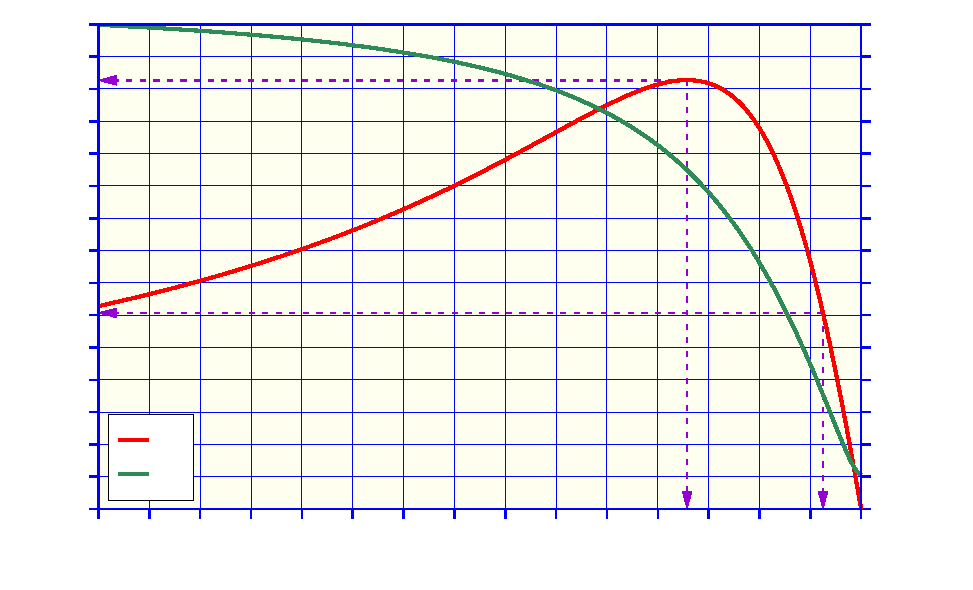
\includegraphics{Cap-Motors-Induccio-Ex4-1}}%
    \gplfronttext
  \end{picture}%
\endgroup

    \end{center}

	Utilitzant les equacions \eqref{eq:cos-fi-mot}, \eqref{eq:mot-S}, \eqref{eq:mot-P}, \eqref{eq:mot-Q} i \eqref{eq:mot-rendim}, representem a continuació dues gràfiques més.
	
	  En la primera s'hi pot veure  l'evolució de les potències mecànica $P\ped{m}$, activa  $P$, reactiva $Q$ i aparent $S$ respecte de la velocitat $n\ped{m}$, indicant-hi també la   velocitat nominal, i el valor nominal de $P\ped{m}$:
	\begin{center}
		\fontsize{10pt}{11pt}\selectfont
		% GNUPLOT: LaTeX picture with Postscript
\begingroup
  \makeatletter
  \providecommand\color[2][]{%
    \GenericError{(gnuplot) \space\space\space\@spaces}{%
      Package color not loaded in conjunction with
      terminal option `colourtext'%
    }{See the gnuplot documentation for explanation.%
    }{Either use 'blacktext' in gnuplot or load the package
      color.sty in LaTeX.}%
    \renewcommand\color[2][]{}%
  }%
  \providecommand\includegraphics[2][]{%
    \GenericError{(gnuplot) \space\space\space\@spaces}{%
      Package graphicx or graphics not loaded%
    }{See the gnuplot documentation for explanation.%
    }{The gnuplot epslatex terminal needs graphicx.sty or graphics.sty.}%
    \renewcommand\includegraphics[2][]{}%
  }%
  \providecommand\rotatebox[2]{#2}%
  \@ifundefined{ifGPcolor}{%
    \newif\ifGPcolor
    \GPcolortrue
  }{}%
  \@ifundefined{ifGPblacktext}{%
    \newif\ifGPblacktext
    \GPblacktexttrue
  }{}%
  % define a \g@addto@macro without @ in the name:
  \let\gplgaddtomacro\g@addto@macro
  % define empty templates for all commands taking text:
  \gdef\gplbacktext{}%
  \gdef\gplfronttext{}%
  \makeatother
  \ifGPblacktext
    % no textcolor at all
    \def\colorrgb#1{}%
    \def\colorgray#1{}%
  \else
    % gray or color?
    \ifGPcolor
      \def\colorrgb#1{\color[rgb]{#1}}%
      \def\colorgray#1{\color[gray]{#1}}%
      \expandafter\def\csname LTw\endcsname{\color{white}}%
      \expandafter\def\csname LTb\endcsname{\color{black}}%
      \expandafter\def\csname LTa\endcsname{\color{black}}%
      \expandafter\def\csname LT0\endcsname{\color[rgb]{1,0,0}}%
      \expandafter\def\csname LT1\endcsname{\color[rgb]{0,1,0}}%
      \expandafter\def\csname LT2\endcsname{\color[rgb]{0,0,1}}%
      \expandafter\def\csname LT3\endcsname{\color[rgb]{1,0,1}}%
      \expandafter\def\csname LT4\endcsname{\color[rgb]{0,1,1}}%
      \expandafter\def\csname LT5\endcsname{\color[rgb]{1,1,0}}%
      \expandafter\def\csname LT6\endcsname{\color[rgb]{0,0,0}}%
      \expandafter\def\csname LT7\endcsname{\color[rgb]{1,0.3,0}}%
      \expandafter\def\csname LT8\endcsname{\color[rgb]{0.5,0.5,0.5}}%
    \else
      % gray
      \def\colorrgb#1{\color{black}}%
      \def\colorgray#1{\color[gray]{#1}}%
      \expandafter\def\csname LTw\endcsname{\color{white}}%
      \expandafter\def\csname LTb\endcsname{\color{black}}%
      \expandafter\def\csname LTa\endcsname{\color{black}}%
      \expandafter\def\csname LT0\endcsname{\color{black}}%
      \expandafter\def\csname LT1\endcsname{\color{black}}%
      \expandafter\def\csname LT2\endcsname{\color{black}}%
      \expandafter\def\csname LT3\endcsname{\color{black}}%
      \expandafter\def\csname LT4\endcsname{\color{black}}%
      \expandafter\def\csname LT5\endcsname{\color{black}}%
      \expandafter\def\csname LT6\endcsname{\color{black}}%
      \expandafter\def\csname LT7\endcsname{\color{black}}%
      \expandafter\def\csname LT8\endcsname{\color{black}}%
    \fi
  \fi
    \setlength{\unitlength}{0.0500bp}%
    \ifx\gptboxheight\undefined%
      \newlength{\gptboxheight}%
      \newlength{\gptboxwidth}%
      \newsavebox{\gptboxtext}%
    \fi%
    \setlength{\fboxrule}{0.5pt}%
    \setlength{\fboxsep}{1pt}%
\begin{picture}(9340.00,5660.00)%
    \gplgaddtomacro\gplbacktext{%
      \colorrgb{0.00,0.00,0.00}%%
      \put(655,787){\makebox(0,0)[r]{\strut{} 0}}%
      \colorrgb{0.00,0.00,0.00}%%
      \put(655,1252){\makebox(0,0)[r]{\strut{} 5}}%
      \colorrgb{0.00,0.00,0.00}%%
      \put(655,1718){\makebox(0,0)[r]{\strut{} 10}}%
      \colorrgb{0.00,0.00,0.00}%%
      \put(655,2183){\makebox(0,0)[r]{\strut{} 15}}%
      \colorrgb{0.00,0.00,0.00}%%
      \put(655,2648){\makebox(0,0)[r]{\strut{} 20}}%
      \colorrgb{0.00,0.00,0.00}%%
      \put(655,3114){\makebox(0,0)[r]{\strut{} 25}}%
      \colorrgb{0.00,0.00,0.00}%%
      \put(655,3579){\makebox(0,0)[r]{\strut{} 30}}%
      \colorrgb{0.00,0.00,0.00}%%
      \put(655,4044){\makebox(0,0)[r]{\strut{} 35}}%
      \colorrgb{0.00,0.00,0.00}%%
      \put(655,4509){\makebox(0,0)[r]{\strut{} 40}}%
      \colorrgb{0.00,0.00,0.00}%%
      \put(655,4975){\makebox(0,0)[r]{\strut{} 45}}%
      \colorrgb{0.00,0.00,0.00}%%
      \put(655,5440){\makebox(0,0)[r]{\strut{} 50}}%
      \colorrgb{0.00,0.00,0.00}%%
      \put(839,481){\makebox(0,0){\strut{} 0}}%
      \colorrgb{0.00,0.00,0.00}%%
      \put(1379,481){\makebox(0,0){\strut{} 100}}%
      \colorrgb{0.00,0.00,0.00}%%
      \put(1919,481){\makebox(0,0){\strut{} 200}}%
      \colorrgb{0.00,0.00,0.00}%%
      \put(2459,481){\makebox(0,0){\strut{} 300}}%
      \colorrgb{0.00,0.00,0.00}%%
      \put(2999,481){\makebox(0,0){\strut{} 400}}%
      \colorrgb{0.00,0.00,0.00}%%
      \put(3539,481){\makebox(0,0){\strut{} 500}}%
      \colorrgb{0.00,0.00,0.00}%%
      \put(4079,481){\makebox(0,0){\strut{} 600}}%
      \colorrgb{0.00,0.00,0.00}%%
      \put(4619,481){\makebox(0,0){\strut{} 700}}%
      \colorrgb{0.00,0.00,0.00}%%
      \put(5159,481){\makebox(0,0){\strut{} 800}}%
      \colorrgb{0.00,0.00,0.00}%%
      \put(5699,481){\makebox(0,0){\strut{} 900}}%
      \colorrgb{0.00,0.00,0.00}%%
      \put(6239,481){\makebox(0,0){\strut{} 1000}}%
      \colorrgb{0.00,0.00,0.00}%%
      \put(6779,481){\makebox(0,0){\strut{} 1100}}%
      \colorrgb{0.00,0.00,0.00}%%
      \put(7319,481){\makebox(0,0){\strut{} 1200}}%
      \colorrgb{0.00,0.00,0.00}%%
      \put(7859,481){\makebox(0,0){\strut{} 1300}}%
      \colorrgb{0.00,0.00,0.00}%%
      \put(8399,481){\makebox(0,0){\strut{} 1400}}%
      \colorrgb{0.00,0.00,0.00}%%
      \put(8939,481){\makebox(0,0){\strut{} 1500}}%
    }%
    \gplgaddtomacro\gplfronttext{%
      \csname LTb\endcsname%%
      \put(255,3113){\rotatebox{-270}{\makebox(0,0){\strut{}$P\ped{m}\, / \,\si{kW}, \quad P\, / \,\si{kW}, \quad Q\, / \,\si{kvar}, \quad S\, / \,\si{kVA}$}}}%
      \csname LTb\endcsname%%
      \put(8993,3113){\rotatebox{-270}{\makebox(0,0){\strut{}}}}%
      \csname LTb\endcsname%%
      \put(4889,153){\makebox(0,0){\strut{}$n\ped{m}\, / \,\si{r/min}$}}%
      \csname LTb\endcsname%%
      \put(4889,5331){\makebox(0,0){\strut{}}}%
      \csname LTb\endcsname%%
      \put(4889,5440){\makebox(0,0){\strut{}}}%
      \csname LTb\endcsname%%
      \put(8435,5189){\makebox(0,0){\strut{}}}%
      \csname LTb\endcsname%%
      \put(8503,5107){\makebox(0,0)[l]{\strut{}$P\ped{m}$}}%
      \csname LTb\endcsname%%
      \put(8503,4779){\makebox(0,0)[l]{\strut{}$P$}}%
      \csname LTb\endcsname%%
      \put(8503,4451){\makebox(0,0)[l]{\strut{}$Q$}}%
      \csname LTb\endcsname%%
      \put(8503,4123){\makebox(0,0)[l]{\strut{}$S$}}%
      \csname LTb\endcsname%%
      \put(1649,1513){\makebox(0,0){$\scriptstyle\SI{9052,8}{W}$}}%
      \csname LTb\endcsname%%
      \put(8442,3114){\rotatebox{-270}{\makebox(0,0){$\scriptstyle\SI{1425}{r/min}$}}}%
    }%
    \gplbacktext
    \put(0,0){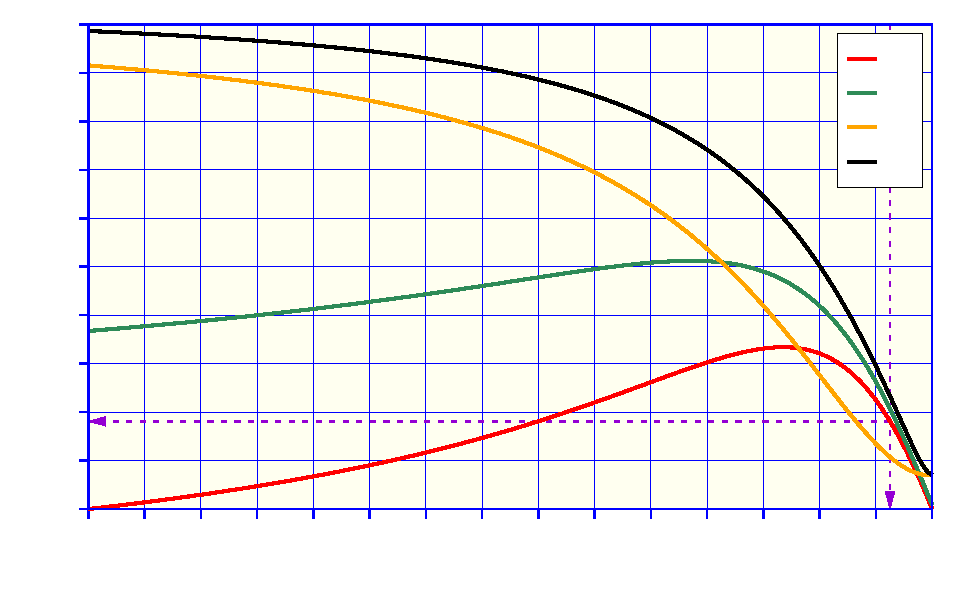
\includegraphics{Cap-Motors-Induccio-Ex4-2}}%
    \gplfronttext
  \end{picture}%
\endgroup

	\end{center}	

	I en la segona s'hi pot veure l'evolució del factor de potència $\cos\varphi$ i del rendiment $\eta$ respecte de la velocitat $n\ped{m}$, indicant-hi també la  velocitat nominal, i els valors nominals de $\cos\varphi$ i $\eta$:
	\begin{center}
	\fontsize{10pt}{11pt}\selectfont
	% GNUPLOT: LaTeX picture with Postscript
\begingroup
  \makeatletter
  \providecommand\color[2][]{%
    \GenericError{(gnuplot) \space\space\space\@spaces}{%
      Package color not loaded in conjunction with
      terminal option `colourtext'%
    }{See the gnuplot documentation for explanation.%
    }{Either use 'blacktext' in gnuplot or load the package
      color.sty in LaTeX.}%
    \renewcommand\color[2][]{}%
  }%
  \providecommand\includegraphics[2][]{%
    \GenericError{(gnuplot) \space\space\space\@spaces}{%
      Package graphicx or graphics not loaded%
    }{See the gnuplot documentation for explanation.%
    }{The gnuplot epslatex terminal needs graphicx.sty or graphics.sty.}%
    \renewcommand\includegraphics[2][]{}%
  }%
  \providecommand\rotatebox[2]{#2}%
  \@ifundefined{ifGPcolor}{%
    \newif\ifGPcolor
    \GPcolortrue
  }{}%
  \@ifundefined{ifGPblacktext}{%
    \newif\ifGPblacktext
    \GPblacktexttrue
  }{}%
  % define a \g@addto@macro without @ in the name:
  \let\gplgaddtomacro\g@addto@macro
  % define empty templates for all commands taking text:
  \gdef\gplbacktext{}%
  \gdef\gplfronttext{}%
  \makeatother
  \ifGPblacktext
    % no textcolor at all
    \def\colorrgb#1{}%
    \def\colorgray#1{}%
  \else
    % gray or color?
    \ifGPcolor
      \def\colorrgb#1{\color[rgb]{#1}}%
      \def\colorgray#1{\color[gray]{#1}}%
      \expandafter\def\csname LTw\endcsname{\color{white}}%
      \expandafter\def\csname LTb\endcsname{\color{black}}%
      \expandafter\def\csname LTa\endcsname{\color{black}}%
      \expandafter\def\csname LT0\endcsname{\color[rgb]{1,0,0}}%
      \expandafter\def\csname LT1\endcsname{\color[rgb]{0,1,0}}%
      \expandafter\def\csname LT2\endcsname{\color[rgb]{0,0,1}}%
      \expandafter\def\csname LT3\endcsname{\color[rgb]{1,0,1}}%
      \expandafter\def\csname LT4\endcsname{\color[rgb]{0,1,1}}%
      \expandafter\def\csname LT5\endcsname{\color[rgb]{1,1,0}}%
      \expandafter\def\csname LT6\endcsname{\color[rgb]{0,0,0}}%
      \expandafter\def\csname LT7\endcsname{\color[rgb]{1,0.3,0}}%
      \expandafter\def\csname LT8\endcsname{\color[rgb]{0.5,0.5,0.5}}%
    \else
      % gray
      \def\colorrgb#1{\color{black}}%
      \def\colorgray#1{\color[gray]{#1}}%
      \expandafter\def\csname LTw\endcsname{\color{white}}%
      \expandafter\def\csname LTb\endcsname{\color{black}}%
      \expandafter\def\csname LTa\endcsname{\color{black}}%
      \expandafter\def\csname LT0\endcsname{\color{black}}%
      \expandafter\def\csname LT1\endcsname{\color{black}}%
      \expandafter\def\csname LT2\endcsname{\color{black}}%
      \expandafter\def\csname LT3\endcsname{\color{black}}%
      \expandafter\def\csname LT4\endcsname{\color{black}}%
      \expandafter\def\csname LT5\endcsname{\color{black}}%
      \expandafter\def\csname LT6\endcsname{\color{black}}%
      \expandafter\def\csname LT7\endcsname{\color{black}}%
      \expandafter\def\csname LT8\endcsname{\color{black}}%
    \fi
  \fi
    \setlength{\unitlength}{0.0500bp}%
    \ifx\gptboxheight\undefined%
      \newlength{\gptboxheight}%
      \newlength{\gptboxwidth}%
      \newsavebox{\gptboxtext}%
    \fi%
    \setlength{\fboxrule}{0.5pt}%
    \setlength{\fboxsep}{1pt}%
\begin{picture}(9340.00,5660.00)%
    \gplgaddtomacro\gplbacktext{%
      \colorrgb{0.00,0.00,0.00}%%
      \put(752,787){\makebox(0,0)[r]{\strut{} 0,0}}%
      \colorrgb{0.00,0.00,0.00}%%
      \put(752,1252){\makebox(0,0)[r]{\strut{} 0,1}}%
      \colorrgb{0.00,0.00,0.00}%%
      \put(752,1718){\makebox(0,0)[r]{\strut{} 0,2}}%
      \colorrgb{0.00,0.00,0.00}%%
      \put(752,2183){\makebox(0,0)[r]{\strut{} 0,3}}%
      \colorrgb{0.00,0.00,0.00}%%
      \put(752,2648){\makebox(0,0)[r]{\strut{} 0,4}}%
      \colorrgb{0.00,0.00,0.00}%%
      \put(752,3114){\makebox(0,0)[r]{\strut{} 0,5}}%
      \colorrgb{0.00,0.00,0.00}%%
      \put(752,3579){\makebox(0,0)[r]{\strut{} 0,6}}%
      \colorrgb{0.00,0.00,0.00}%%
      \put(752,4044){\makebox(0,0)[r]{\strut{} 0,7}}%
      \colorrgb{0.00,0.00,0.00}%%
      \put(752,4509){\makebox(0,0)[r]{\strut{} 0,8}}%
      \colorrgb{0.00,0.00,0.00}%%
      \put(752,4975){\makebox(0,0)[r]{\strut{} 0,9}}%
      \colorrgb{0.00,0.00,0.00}%%
      \put(752,5440){\makebox(0,0)[r]{\strut{} 1,0}}%
      \colorrgb{0.00,0.00,0.00}%%
      \put(936,481){\makebox(0,0){\strut{} 0}}%
      \colorrgb{0.00,0.00,0.00}%%
      \put(1470,481){\makebox(0,0){\strut{} 100}}%
      \colorrgb{0.00,0.00,0.00}%%
      \put(2003,481){\makebox(0,0){\strut{} 200}}%
      \colorrgb{0.00,0.00,0.00}%%
      \put(2537,481){\makebox(0,0){\strut{} 300}}%
      \colorrgb{0.00,0.00,0.00}%%
      \put(3070,481){\makebox(0,0){\strut{} 400}}%
      \colorrgb{0.00,0.00,0.00}%%
      \put(3604,481){\makebox(0,0){\strut{} 500}}%
      \colorrgb{0.00,0.00,0.00}%%
      \put(4137,481){\makebox(0,0){\strut{} 600}}%
      \colorrgb{0.00,0.00,0.00}%%
      \put(4671,481){\makebox(0,0){\strut{} 700}}%
      \colorrgb{0.00,0.00,0.00}%%
      \put(5204,481){\makebox(0,0){\strut{} 800}}%
      \colorrgb{0.00,0.00,0.00}%%
      \put(5738,481){\makebox(0,0){\strut{} 900}}%
      \colorrgb{0.00,0.00,0.00}%%
      \put(6271,481){\makebox(0,0){\strut{} 1000}}%
      \colorrgb{0.00,0.00,0.00}%%
      \put(6805,481){\makebox(0,0){\strut{} 1100}}%
      \colorrgb{0.00,0.00,0.00}%%
      \put(7338,481){\makebox(0,0){\strut{} 1200}}%
      \colorrgb{0.00,0.00,0.00}%%
      \put(7872,481){\makebox(0,0){\strut{} 1300}}%
      \colorrgb{0.00,0.00,0.00}%%
      \put(8405,481){\makebox(0,0){\strut{} 1400}}%
      \colorrgb{0.00,0.00,0.00}%%
      \put(8939,481){\makebox(0,0){\strut{} 1500}}%
    }%
    \gplgaddtomacro\gplfronttext{%
      \csname LTb\endcsname%%
      \put(255,3113){\rotatebox{-270}{\makebox(0,0){\strut{}$\cos\varphi, \quad \eta$}}}%
      \csname LTb\endcsname%%
      \put(8993,3113){\rotatebox{-270}{\makebox(0,0){\strut{}}}}%
      \csname LTb\endcsname%%
      \put(4937,153){\makebox(0,0){\strut{}$n\ped{m}\, / \,\si{r/min}$}}%
      \csname LTb\endcsname%%
      \put(4937,5331){\makebox(0,0){\strut{}}}%
      \csname LTb\endcsname%%
      \put(4937,5440){\makebox(0,0){\strut{}}}%
      \csname LTb\endcsname%%
      \put(7052,1786){\makebox(0,0){\strut{}}}%
      \csname LTb\endcsname%%
      \put(6975,1704){\makebox(0,0)[l]{\strut{}$\cos\varphi$}}%
      \csname LTb\endcsname%%
      \put(6975,1376){\makebox(0,0)[l]{\strut{}$\eta$}}%
      \csname LTb\endcsname%%
      \put(8448,1718){\rotatebox{-270}{\makebox(0,0){$\scriptstyle\SI{1425}{r/min}$}}}%
      \csname LTb\endcsname%%
      \put(1736,5021){\makebox(0,0){$\scriptstyle\num{0,887}$}}%
      \csname LTb\endcsname%%
      \put(1736,4742){\makebox(0,0){$\scriptstyle\num{0,876}$}}%
    }%
    \gplbacktext
    \put(0,0){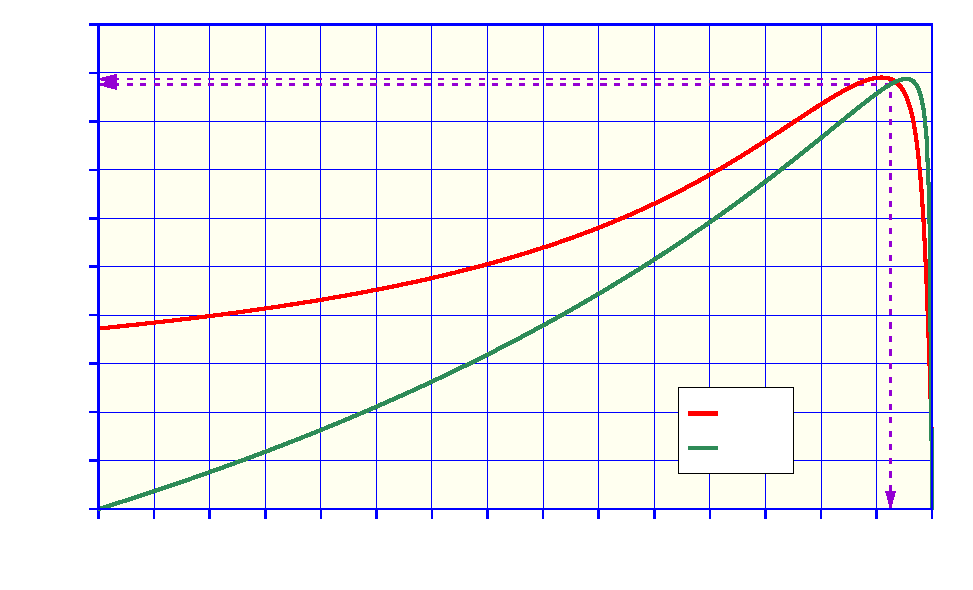
\includegraphics{Cap-Motors-Induccio-Ex4-3}}%
    \gplfronttext
  \end{picture}%
\endgroup

	\end{center}	

\end{exemple}

\subsection{Tensió desequilibrada}\label{sec:mot-tens-deseq}\index{motors d'inducció!tensió desequilibrada}

Un motor consumeix el corrent nominal quan subministra la potència mecànica nominal girant a la velocitat nominal, i està alimentat a la tensió nominal. Per tal que això sigui cert, la tensió d'alimentació trifàsica ha de ser equilibrada.

Quan la tensió trifàsica d'alimentació és desequilibrada, es creen tensions de seqüència directa i inversa, les quals  produeixen corrents de la seqüència corresponent. El corrent de seqüència inversa creix ràpidament inclús per a valors baixos de  la tensió de seqüència inversa; aquest corrent genera una calor addicional que el motor haurà d'evacuar, i una possible actuació de les proteccions elèctriques del motor.

En la Figura \vref{pic:mot-esq-equiv-seq-neg} es representa l'esquema equivalent per fase de seqüència inversa d'un   motor d'inducció:

\begin{center}
	\input{Imatges/Cap-Motors-Induccio-Esq-Equiv-Seq-Neg.pdf_tex}
	\captionof{figure}{Esquema elèctric equivalent per fase de seqüència inversa d'un motor}
	\label{pic:mot-esq-equiv-seq-neg}
\end{center}

Les tensions i corrents tenen el subíndex «2» afegit per indicar que són de seqüència inversa. Com es pot veure, la diferència amb l'esquema equivalent de seqüència directa (Figura \vref{pic:mot-esq-equiv}) rau en la part resistiva del rotor. En aquest cas la resistència vista per l'estator és $\frac{R_2}{2-s}$; aquesta resistència vista per l'estator se separa igualment en dues parts: $R_2$ i $-\frac{1-s}{2-s} R_2$. El corrent de seqüència inversa, de forma anàloga al corrent de seqüència directa,  origina en el rotor unes pèrdues proporcionals a $R_2$, i un parell proporcional a $-\frac{1-s}{2-s} R_2$, el qual en ser negatiu s'oposa al parell creat pel corrent de seqüència directa; aquest parell invers és, tanmateix, molt petit comparat amb el parell directe a la velocitat nominal del motor.

Donat que els motors no tenen un punt neutre connectat a terra, no hi poden haver corrents homopolars, i per tant no existeix cap esquema equivalent de seqüència homopolar del motor.

A partir de l'esquema de la figura \vref{pic:mot-esq-equiv-seq-neg} es poden obtenir totes les equacions de seqüència inversa d'impedàncies, corrents, tensions, potències i parells, tal com s'ha fet en les seccions \ref{sec:mot-u-c-i} i \ref{sec:mot-p-t} per a la seqüència directa. Es donen a continuació a tall d'exemple, les equacions en funció de $s$ de la impedància total de seqüència inversa del motor $\cmplx{Z}\ped{mot,2}(s)$ i del corrent de fase de seqüència inversa de l'estator $\cmplx{I}_{1,2}(s)$:
\begin{align}
	\cmplx{Z}\ped{mot,2}(s) &= R_1 + \ju X_1 + \frac{\cmplx{Z}_0 \left( \dfrac{R_2}{2-s} + \ju X_2\right)}{\cmplx{Z}_0 +  \dfrac{R_2}{2-s} + \ju X_2}\label{eq:mot-Zmot-inv}\\
	\cmplx{I}_{1,2}(s) &= \frac{\cmplx{U}_{1,2}}{\cmplx{Z}\ped{mot,2}(s)}\label{eq:mot-I1-inv}
\end{align}

En l'equació anterior, $\cmplx{U}_{1,2}$ és la tensió  fase--neutre de seqüència inversa aplicada a l’estator.

A causa dels valors usuals de les resistències i reactàncies dels motors trifàsics, es compleix de forma aproximada que la impedància de seqüència inversa del motor, a lliscament nominal,  és igual a la impedància d'arrencada de seqüència directa del motor, segons l'equació \eqref{eq:z-mot-arr}:
\begin{equation}
	\cmplx{Z}\ped{mot,2}(s\ped{n}) \approx \cmplx{Z}\ped{mot,arr,1}\label{eq:Zarr-aprox-Z2}
\end{equation}


\begin{exemple}[Motor alimentat amb tensió desequilibrada]\label{ex:mot-tens-deseq}
	\addcontentsxms{Motor alimentat amb tensió desequilibrada}
	Partim del mateix motor utilitzat en l'exemple \vref{ex:mot}, però alimentat amb un sistema de tensions desequilibrades de valor: $U\ped{AB} =
	\qty{399}{V}$, $U\ped{BC} = \qty{370}{V}$ i
	$U\ped{CA} = \qty{370}{V}$. Es tracta de trobar el corrent absorbit pel motor a la velocitat nominal.
	
	Transformarem primer les tensions $U\ped{AB}$, $U\ped{BC}$ i $U\ped{CA}$ en tres fasors; seguint el mètode de l'exemple \vref{ex:comp-sim}, trobem:
	\begin{align*}
		\cmplx{U}\ped{AB} &= \qtypd{399}{0}{V} \\
		\cmplx{U}\ped{BC} &= \qtypd{370}{-122,63}{V} \\
		\cmplx{U}\ped{CA} &= \qtypd{370}{122,63}{V}
	\end{align*}
	
	Calculem a continuació les components simètriques d'aquestes tres tensions fase--fase, utilitzant les equacions
	\eqref{eq:c_sim_c2}, \eqref{eq:c_sim_a2} i \eqref{eq:c_sim_b2}:
	\begin{align*}
	\cmplx{U}\ped{AB,1} &= \frac{1}{3} \big(
	\qtypd{399}{0}{V} + \numpd{1}{120} \times \qtypd{370}{-122,63}{V} +
	\numpd{1}{240} \times \qtypd{370}{122,63}{V}\big) = \qtypd{379,41}{0}{V} \\[1ex]
	\cmplx{U}\ped{AB,2} &= \frac{1}{3} \big(
	\qtypd{399}{0}{V} + \numpd{1}{240} \times \qtypd{370}{-122,63}{V} +
	\numpd{1}{120} \times \qtypd{370}{122,63}{V} \big) = \qtypd{19,59}{0}{V} \\[1ex]
	\cmplx{U}\ped{AB,0} &= \frac{1}{3} \big(
	\qtypd{399}{0}{V} + \qtypd{370}{-122,63}{V} + \qtypd{370}{122,63}{V}\big) = \qty{0}{V}
	\end{align*}
	
	Com era d'esperar, la component homopolar és nuŀla.	 Trobem ara les components directa i inversa
	de les tensions fase--neutre, utilitzant les equacions
	\eqref{eq:c_sim_a3} i \eqref{eq:c_sim_b3}:
	\begin{align*}
	\cmplx{U}\ped{AN,1} &=
	\frac{\cmplx{U}\ped{AB,1}}{\sqrt{3}_{\angle\ang{30}}} =
	\frac{\qtypd{379,41}{0}{V}}{\sqrt{3}_{\angle\ang{30}}} =
	\qtypd{219,05}{-30}{V} \\[1ex]
	\cmplx{U}\ped{AN,2} &=
	\frac{\cmplx{U}\ped{AB,2}}{\sqrt{3}_{\angle\ang{-30}}} =
	\frac{\qtypd{19,59}{0}{V}}{\sqrt{3}_{\angle\ang{-30}}} =
	\qtypd{11,31}{30}{V} 
	\end{align*}
	
	El valor relatiu de la tensió de seqüència inversa respecte de la tensió de seqüència directa és:
	\[
		\frac{U\ped{AN,2}}{U\ped{AN,1}} = \frac{\qty{11,31}{V}}{\qty{219,05}{V}} = 0{,}052
	\]
	
	Calculem a continuació les impedàncies dels circuits directe i invers, a lliscament nominal. La impedància transversal $\cmplx{Z}_0$ ja s'ha calculat en l'exemple \ref{ex:mot}: $ \cmplx{Z}_0 =  \complexqty{4,390+j39,512}{\ohm} $. Utilitzant ara les equacions \eqref{eq:mot-Zmot} i \eqref{eq:mot-Zmot-inv} amb el valor $s=0{,}05$, trobem les impedàncies nominals:
	\begin{align*}
		\cmplx{Z}\ped{mot,n,1} &= \complexqty{11,004+j5,718}{\ohm} \\
		\cmplx{Z}\ped{mot,n,2} &= \complexqty{0,805+j2,712}{\ohm}
	\end{align*}
	
	El valor de la impedància d'arrencada de seqüència directa el trobem utilitzant l'equació \eqref{eq:z-mot-arr}:
	\[
		\cmplx{Z}\ped{mot,arr,1} = \complexqty{1,091+j2,717}{\ohm}
	\]
	
	Es pot comprovar que es compleix l'equació \eqref{eq:Zarr-aprox-Z2}, és a dir: $\cmplx{Z}\ped{mot,n,2} \approx \cmplx{Z}\ped{mot,arr,1}$.
	
	Calculem ara amb el valor $s=0{,}05$, els corrents nominals del motor de seqüència directa i inversa utilitzant les equacions \eqref{eq:mot-I1} i \eqref{eq:mot-I1-inv}:
	\begin{align*}
		\cmplx{I}\ped{1,n,1} &=  \frac{\qtypd{219,05}{-30}{V}}{\complexqty{11,004+j5,718}{\ohm}} = \qtypd{17,67}{-57,46}{A} \\[1ex] 
		\cmplx{I}\ped{1,n,2} &= \frac{\qtypd{11,31}{30}{V}}{\complexqty{0,805+j2,712}{\ohm}} = \qtypd{4,00}{-43,47}{A}
	\end{align*}
	
	El valor relatiu del corrent de seqüència inversa respecte del corrent de seqüència directa és:
	\[
		\frac{I\ped{1,n,2}}{I\ped{1,n,1}} = \frac{\qty{4,00}{A}}{\qty{17,67}{A}} = 0{,}226
	\]	
	
	Es pot veure doncs, que una tensió de seqüència negativa petita (de l'ordre del 5,2 \% de la tensió de seqüència positiva), origina un corrent de seqüència negativa elevat (de l'ordre del 22,6 \% del corrent de seqüència positiva). 
	
	Calculem finalment els corrents nominals de les tres fases $\cmplx{I}\ped{1,n,A}$, $\cmplx{I}\ped{1,n,B}$ i $\cmplx{I}\ped{1,n,C}$, utilitzant les equacions \eqref{eq:c_sim_a},
	\eqref{eq:c_sim_b} i \eqref{eq:c_sim_c}, tenint en compte que el corrent de seqüència homopolar és nul:
	\begin{align*}
		\cmplx{I}\ped{1,n,A} &= \qty{0}{A} + \qtypd{17,67}{-57,46}{A} +
		\qtypd{4,00}{-43,47}{A}  =
		\qtypd{21,57}{-54,89}{A} \\[1ex]
		\cmplx{I}\ped{1,n,B} &= \qty{0}{A} + \numpd{1}{240} \times
		\qtypd{17,67}{-57,46}{A} + \numpd{1}{120} \times
		\qtypd{4,00}{-43,47}{A}  =
		\qtypd{17,00}{169,48}{A}    \\[1ex]
		\cmplx{I}\ped{1,n,C} &= \qty{0}{A} + \numpd{1}{120} \times
		\qtypd{17,67}{-57,46}{A} +
		\numpd{1}{240} \times \qtypd{4,00}{-43,47}{A}  =
		\qtypd{15,16}{73,48}{A}
\end{align*}
	
\end{exemple}
	

\subsection{Tensió i potència reduïda}\label{sec:mot-tens-pot-red}

En general, el principal objectiu de les equacions desenvolupades fins ara ha estat  el càlcul de les variables associades al motor (tensió, corrent, parell, etc.) en condicions nominals.

Hi ha, tanmateix, alguns casos del funcionament del motor fora de les condicions nominals, que també són d'interès: 
\begin{itemize}
	\item  Motor alimentat a tensió nominal que subministra una potència reduïda.
	\item  Motor alimentat a tensió reduïda que arrossega la càrrega nominal.
	\begin{itemize}
		\item Solució aproximada: suposa que la potència mecànica nominal es manté constant.
		\item Solució exacta: requereix el coneixement de la corba parell-velocitat de la càrrega.
	\end{itemize}	
	\item Arrencada d'un motor a tensió reduïda, deguda a la caiguda de tensió originada pel corrent d'arrencada mateix.
\end{itemize}

En aquests casos les equacions que ens interessen són les \eqref{eq:Pm-I2-U1} i \eqref{eq:Tm-Prot-ws}, les quals relacionen la potència mecànica $P\ped{m}(s)$ i el parell mecànic $T\ped{m}(s)$ amb la tensió $U_1$ i el lliscament $s$. Si substituïm en aquestes equacions $Y\ped{eq}(s)$ pel seu valor, tenim:
\begin{subequations}
	\begin{align}
	P\ped{m}(s) &= \frac{3(1-s) R_2 U_1^2}{s} \left( \frac{Z_0}{\big|R_1 + \ju X_1 + \cmplx{Z}_0\big| \left|\cmplx{Z}\ped{Th} + \dfrac{R_2}{s} + \ju X_2\right|} \right)^2 \label{eq:Pm-U1-Yeq} \\
	T\ped{m}(s) &= \frac{3 R_2 U_1^2}{s\omega\ped{m,sinc}}  \left( \frac{Z_0}{\big|R_1 + \ju X_1 + \cmplx{Z}_0\big| \left|\cmplx{Z}\ped{Th} + \dfrac{R_2}{s} + \ju X_2\right|} \right)^2\label{eq:Tm-U1-Yeq}
	\end{align}
\end{subequations}

	
\subsubsection{Tensió nominal i potència reduïda}\index{motors d'inducció!potència reduïda}	

Si tot mantenint la tensió nominal la potència de la càrrega disminueix, el lliscament disminueix (és a dir, la velocitat augmenta), i el corrent del motor disminueix.
	
Si en l'equació \eqref{eq:Pm-U1-Yeq} fixem $U_1$ al seu valor nominal i  $P\ped{m}$ al  valor reduït existent,  la podrem resoldre obtenint el valor de $s$ corresponent  a aquesta situació. Un cop tenim $s$, podem trobar la intensitat del motor $I_1$ utilitzant les equacions \eqref{eq:mot-Zmot} i \eqref{eq:mot-I1}. És clar que també podem trobar qualsevol altre valor del motor, com  ara el factor de potència o el rendiment, utilitzant les equacions pertinents.


\begin{exemple}[Motor connectat a una càrrega  reduïda]
	\addcontentsxms{Motor connectat a una càrrega  reduïda}
	Partim del mateix motor utilitzat en l'exemple \vref{ex:mot}, però connectat a una càrrega igual  al 50 \% de la potència mecànica nominal. Es tracta de trobar el corrent, el factor de potència i el rendiment del motor en aquestes condicions.

	La tensió  fase--neutre  nominal, calculada  en l'exemple \ref{ex:mot}, val: 
	\[
		U\ped{n} = \qty{219,393}{V}
	\]
	
	El 50 \% de la potència mecànica nominal, calculada  en l'exemple \ref{ex:mot}, val:
	\[
		P\ped{m} =  0{,}5\times\qty{9052,8}{W} = \qty{4526,4}{W}
	\]

	Els valors de $\cmplx{Z}_0$ i  $\cmplx{Z}\ped{Th}$, els quals no depenen del lliscament, també s'han calculat en  l'exemple \ref{ex:mot}, i valen:
	\begin{align*}
		\cmplx{Z}_0 &=  \complexqty{4,390+j39,512}{\ohm} \\[1ex]
		\cmplx{Z}\ped{Th} &= \complexqty{0,470+j1,448}{\ohm} 
	\end{align*}
	
	A continuació  substituïm aquests valors en l'equació \eqref{eq:Pm-U1-Yeq} i la resolem.  Aquesta equació és clarament no lineal, i per tal de resoldre-la cal utilitzar programes de càlcul o mètodes numèrics, com ara els explicats en l'apèndix \ref{sec:func-no-lin}. La solució és:
	\[
		s = 0{,}023
	\]
	Finalment, utilitzant les equacions \eqref{eq:mot-Zmot} i \eqref{eq:mot-I1} amb $s  = 0{,}023$,  trobem el corrent del motor:
	\begin{align*}
	\cmplx{Z}\ped{mot}(0{,}023) &=  \complexqty{18,015+j13,510}{\ohm} \\[0.5ex]
	I_1(0{,}023) &= \frac{\qty{219,393}{V}}{|\complexqty{18,015+j13,510}{\ohm}|} = \qty{9,7}{A}
	\end{align*}
	
	La relació entre aquest  corrent i el corrent nominal a tensió i potència nominals, calculat en l'exemple \ref{ex:mot}, és
	\[
	\frac{I_1(0{,}023)}{I\ped{1,n}} = \frac{\qty{9,7}{A}}{\qty{17,7}{A}} = 0{,}6
	\]
	Utilitzant les equacions  \eqref{eq:cos-fi-mot} i \eqref{eq:mot-rendim} amb $s  = 0{,}023$, podem calcular els valors del factor de potència i del rendiment:
	\begin{align*}
		\cos\varphi(0{,}023) &=  0{,}800 \\
		\eta(0{,}023) &=  0{,}882
	\end{align*}	
	Representem a continuació la gràfica de l'evolució del lliscament $s$ i del corrent $I_1$ respecte de la relació entre la potència mecànica proporcionada i la potència mecànica nominal $P\ped{m}/P\ped{m,n}$, indicant-hi els valors del lliscament i de la intensitat calculats anteriorment:
	\begin{center}
		% GNUPLOT: LaTeX picture with Postscript
\begingroup
  \makeatletter
  \providecommand\color[2][]{%
    \GenericError{(gnuplot) \space\space\space\@spaces}{%
      Package color not loaded in conjunction with
      terminal option `colourtext'%
    }{See the gnuplot documentation for explanation.%
    }{Either use 'blacktext' in gnuplot or load the package
      color.sty in LaTeX.}%
    \renewcommand\color[2][]{}%
  }%
  \providecommand\includegraphics[2][]{%
    \GenericError{(gnuplot) \space\space\space\@spaces}{%
      Package graphicx or graphics not loaded%
    }{See the gnuplot documentation for explanation.%
    }{The gnuplot epslatex terminal needs graphicx.sty or graphics.sty.}%
    \renewcommand\includegraphics[2][]{}%
  }%
  \providecommand\rotatebox[2]{#2}%
  \@ifundefined{ifGPcolor}{%
    \newif\ifGPcolor
    \GPcolortrue
  }{}%
  \@ifundefined{ifGPblacktext}{%
    \newif\ifGPblacktext
    \GPblacktexttrue
  }{}%
  % define a \g@addto@macro without @ in the name:
  \let\gplgaddtomacro\g@addto@macro
  % define empty templates for all commands taking text:
  \gdef\gplbacktext{}%
  \gdef\gplfronttext{}%
  \makeatother
  \ifGPblacktext
    % no textcolor at all
    \def\colorrgb#1{}%
    \def\colorgray#1{}%
  \else
    % gray or color?
    \ifGPcolor
      \def\colorrgb#1{\color[rgb]{#1}}%
      \def\colorgray#1{\color[gray]{#1}}%
      \expandafter\def\csname LTw\endcsname{\color{white}}%
      \expandafter\def\csname LTb\endcsname{\color{black}}%
      \expandafter\def\csname LTa\endcsname{\color{black}}%
      \expandafter\def\csname LT0\endcsname{\color[rgb]{1,0,0}}%
      \expandafter\def\csname LT1\endcsname{\color[rgb]{0,1,0}}%
      \expandafter\def\csname LT2\endcsname{\color[rgb]{0,0,1}}%
      \expandafter\def\csname LT3\endcsname{\color[rgb]{1,0,1}}%
      \expandafter\def\csname LT4\endcsname{\color[rgb]{0,1,1}}%
      \expandafter\def\csname LT5\endcsname{\color[rgb]{1,1,0}}%
      \expandafter\def\csname LT6\endcsname{\color[rgb]{0,0,0}}%
      \expandafter\def\csname LT7\endcsname{\color[rgb]{1,0.3,0}}%
      \expandafter\def\csname LT8\endcsname{\color[rgb]{0.5,0.5,0.5}}%
    \else
      % gray
      \def\colorrgb#1{\color{black}}%
      \def\colorgray#1{\color[gray]{#1}}%
      \expandafter\def\csname LTw\endcsname{\color{white}}%
      \expandafter\def\csname LTb\endcsname{\color{black}}%
      \expandafter\def\csname LTa\endcsname{\color{black}}%
      \expandafter\def\csname LT0\endcsname{\color{black}}%
      \expandafter\def\csname LT1\endcsname{\color{black}}%
      \expandafter\def\csname LT2\endcsname{\color{black}}%
      \expandafter\def\csname LT3\endcsname{\color{black}}%
      \expandafter\def\csname LT4\endcsname{\color{black}}%
      \expandafter\def\csname LT5\endcsname{\color{black}}%
      \expandafter\def\csname LT6\endcsname{\color{black}}%
      \expandafter\def\csname LT7\endcsname{\color{black}}%
      \expandafter\def\csname LT8\endcsname{\color{black}}%
    \fi
  \fi
    \setlength{\unitlength}{0.0500bp}%
    \ifx\gptboxheight\undefined%
      \newlength{\gptboxheight}%
      \newlength{\gptboxwidth}%
      \newsavebox{\gptboxtext}%
    \fi%
    \setlength{\fboxrule}{0.5pt}%
    \setlength{\fboxsep}{1pt}%
\begin{picture}(9340.00,5660.00)%
    \gplgaddtomacro\gplbacktext{%
      \colorrgb{0.00,0.00,0.00}%%
      \put(1018,787){\makebox(0,0)[r]{\strut{} 0,000}}%
      \colorrgb{0.00,0.00,0.00}%%
      \put(1018,1252){\makebox(0,0)[r]{\strut{} 0,005}}%
      \colorrgb{0.00,0.00,0.00}%%
      \put(1018,1718){\makebox(0,0)[r]{\strut{} 0,010}}%
      \colorrgb{0.00,0.00,0.00}%%
      \put(1018,2183){\makebox(0,0)[r]{\strut{} 0,015}}%
      \colorrgb{0.00,0.00,0.00}%%
      \put(1018,2648){\makebox(0,0)[r]{\strut{} 0,020}}%
      \colorrgb{0.00,0.00,0.00}%%
      \put(1018,3114){\makebox(0,0)[r]{\strut{} 0,025}}%
      \colorrgb{0.00,0.00,0.00}%%
      \put(1018,3579){\makebox(0,0)[r]{\strut{} 0,030}}%
      \colorrgb{0.00,0.00,0.00}%%
      \put(1018,4044){\makebox(0,0)[r]{\strut{} 0,035}}%
      \colorrgb{0.00,0.00,0.00}%%
      \put(1018,4509){\makebox(0,0)[r]{\strut{} 0,040}}%
      \colorrgb{0.00,0.00,0.00}%%
      \put(1018,4975){\makebox(0,0)[r]{\strut{} 0,045}}%
      \colorrgb{0.00,0.00,0.00}%%
      \put(1018,5440){\makebox(0,0)[r]{\strut{} 0,050}}%
      \colorrgb{0.00,0.00,0.00}%%
      \put(1202,481){\makebox(0,0){\strut{} 0,0}}%
      \colorrgb{0.00,0.00,0.00}%%
      \put(1908,481){\makebox(0,0){\strut{} 0,1}}%
      \colorrgb{0.00,0.00,0.00}%%
      \put(2613,481){\makebox(0,0){\strut{} 0,2}}%
      \colorrgb{0.00,0.00,0.00}%%
      \put(3319,481){\makebox(0,0){\strut{} 0,3}}%
      \colorrgb{0.00,0.00,0.00}%%
      \put(4024,481){\makebox(0,0){\strut{} 0,4}}%
      \colorrgb{0.00,0.00,0.00}%%
      \put(4730,481){\makebox(0,0){\strut{} 0,5}}%
      \colorrgb{0.00,0.00,0.00}%%
      \put(5435,481){\makebox(0,0){\strut{} 0,6}}%
      \colorrgb{0.00,0.00,0.00}%%
      \put(6141,481){\makebox(0,0){\strut{} 0,7}}%
      \colorrgb{0.00,0.00,0.00}%%
      \put(6846,481){\makebox(0,0){\strut{} 0,8}}%
      \colorrgb{0.00,0.00,0.00}%%
      \put(7551,481){\makebox(0,0){\strut{} 0,9}}%
      \colorrgb{0.00,0.00,0.00}%%
      \put(8257,481){\makebox(0,0){\strut{} 1,0}}%
      \colorrgb{0.00,0.00,0.00}%%
      \put(8441,787){\makebox(0,0)[l]{\strut{} 0}}%
      \colorrgb{0.00,0.00,0.00}%%
      \put(8441,1252){\makebox(0,0)[l]{\strut{} 2}}%
      \colorrgb{0.00,0.00,0.00}%%
      \put(8441,1718){\makebox(0,0)[l]{\strut{} 4}}%
      \colorrgb{0.00,0.00,0.00}%%
      \put(8441,2183){\makebox(0,0)[l]{\strut{} 6}}%
      \colorrgb{0.00,0.00,0.00}%%
      \put(8441,2648){\makebox(0,0)[l]{\strut{} 8}}%
      \colorrgb{0.00,0.00,0.00}%%
      \put(8441,3114){\makebox(0,0)[l]{\strut{} 10}}%
      \colorrgb{0.00,0.00,0.00}%%
      \put(8441,3579){\makebox(0,0)[l]{\strut{} 12}}%
      \colorrgb{0.00,0.00,0.00}%%
      \put(8441,4044){\makebox(0,0)[l]{\strut{} 14}}%
      \colorrgb{0.00,0.00,0.00}%%
      \put(8441,4509){\makebox(0,0)[l]{\strut{} 16}}%
      \colorrgb{0.00,0.00,0.00}%%
      \put(8441,4975){\makebox(0,0)[l]{\strut{} 18}}%
      \colorrgb{0.00,0.00,0.00}%%
      \put(8441,5440){\makebox(0,0)[l]{\strut{} 20}}%
    }%
    \gplgaddtomacro\gplfronttext{%
      \csname LTb\endcsname%%
      \put(291,3113){\makebox(0,0){\strut{}$s$}}%
      \csname LTb\endcsname%%
      \put(8938,3113){\rotatebox{-270}{\makebox(0,0){\strut{}$I_1\, / \,\si{A}$}}}%
      \csname LTb\endcsname%%
      \put(4729,153){\makebox(0,0){\strut{}$P\ped{m}/P\ped{m,n}$}}%
      \csname LTb\endcsname%%
      \put(4729,5331){\makebox(0,0){\strut{}}}%
      \csname LTb\endcsname%%
      \put(4729,5440){\makebox(0,0){\strut{}}}%
      \csname LTb\endcsname%%
      \put(7801,1530){\makebox(0,0){\strut{}}}%
      \csname LTb\endcsname%%
      \put(7918,1448){\makebox(0,0)[l]{\strut{}$s$}}%
      \csname LTb\endcsname%%
      \put(7918,1120){\makebox(0,0)[l]{\strut{}$I_1$}}%
      \csname LTb\endcsname%%
      \put(4624,1485){\rotatebox{-270}{\makebox(0,0){$\scriptstyle\num{0.5}$}}}%
      \csname LTb\endcsname%%
      \put(7199,3207){\makebox(0,0){$\scriptstyle\SI{9,7}{A}$}}%
      \csname LTb\endcsname%%
      \put(2260,2974){\makebox(0,0){$\scriptstyle\num{0,023}$}}%
    }%
    \gplbacktext
    \put(0,0){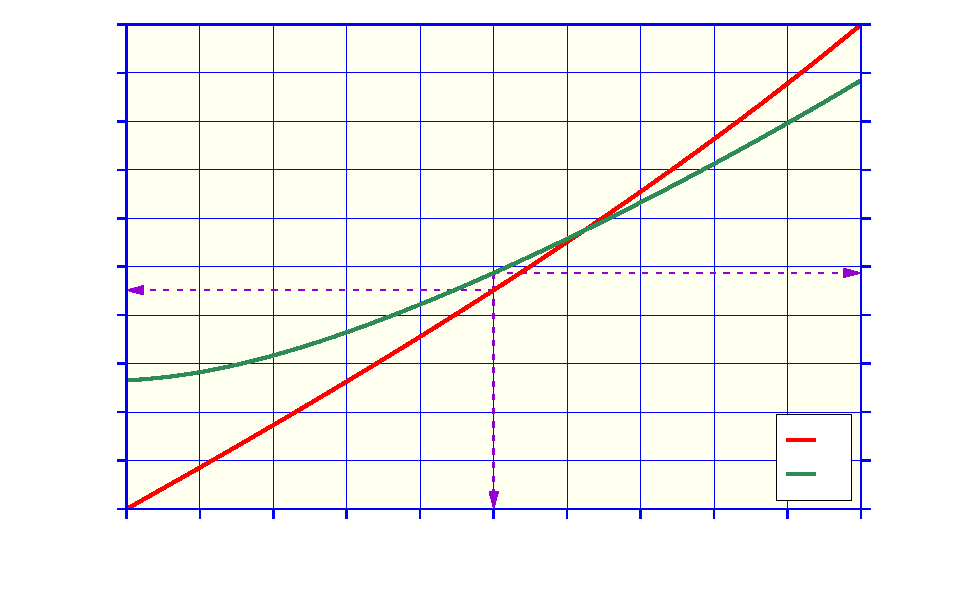
\includegraphics{Cap-Motors-Induccio-Ex6-1}}%
    \gplfronttext
  \end{picture}%
\endgroup

	\end{center}

	Per acabar, representem  la gràfica de l'evolució del factor de potència $\cos\varphi$ i del rendiment $\eta$  respecte de la relació entre la potència mecànica proporcionada i la potència mecànica nominal $P\ped{m}/P\ped{m,n}$, indicant-hi també els valors del factor de potència i del rendiment calculats anteriorment:
	\begin{center}
		% GNUPLOT: LaTeX picture with Postscript
\begingroup
  \makeatletter
  \providecommand\color[2][]{%
    \GenericError{(gnuplot) \space\space\space\@spaces}{%
      Package color not loaded in conjunction with
      terminal option `colourtext'%
    }{See the gnuplot documentation for explanation.%
    }{Either use 'blacktext' in gnuplot or load the package
      color.sty in LaTeX.}%
    \renewcommand\color[2][]{}%
  }%
  \providecommand\includegraphics[2][]{%
    \GenericError{(gnuplot) \space\space\space\@spaces}{%
      Package graphicx or graphics not loaded%
    }{See the gnuplot documentation for explanation.%
    }{The gnuplot epslatex terminal needs graphicx.sty or graphics.sty.}%
    \renewcommand\includegraphics[2][]{}%
  }%
  \providecommand\rotatebox[2]{#2}%
  \@ifundefined{ifGPcolor}{%
    \newif\ifGPcolor
    \GPcolortrue
  }{}%
  \@ifundefined{ifGPblacktext}{%
    \newif\ifGPblacktext
    \GPblacktexttrue
  }{}%
  % define a \g@addto@macro without @ in the name:
  \let\gplgaddtomacro\g@addto@macro
  % define empty templates for all commands taking text:
  \gdef\gplbacktext{}%
  \gdef\gplfronttext{}%
  \makeatother
  \ifGPblacktext
    % no textcolor at all
    \def\colorrgb#1{}%
    \def\colorgray#1{}%
  \else
    % gray or color?
    \ifGPcolor
      \def\colorrgb#1{\color[rgb]{#1}}%
      \def\colorgray#1{\color[gray]{#1}}%
      \expandafter\def\csname LTw\endcsname{\color{white}}%
      \expandafter\def\csname LTb\endcsname{\color{black}}%
      \expandafter\def\csname LTa\endcsname{\color{black}}%
      \expandafter\def\csname LT0\endcsname{\color[rgb]{1,0,0}}%
      \expandafter\def\csname LT1\endcsname{\color[rgb]{0,1,0}}%
      \expandafter\def\csname LT2\endcsname{\color[rgb]{0,0,1}}%
      \expandafter\def\csname LT3\endcsname{\color[rgb]{1,0,1}}%
      \expandafter\def\csname LT4\endcsname{\color[rgb]{0,1,1}}%
      \expandafter\def\csname LT5\endcsname{\color[rgb]{1,1,0}}%
      \expandafter\def\csname LT6\endcsname{\color[rgb]{0,0,0}}%
      \expandafter\def\csname LT7\endcsname{\color[rgb]{1,0.3,0}}%
      \expandafter\def\csname LT8\endcsname{\color[rgb]{0.5,0.5,0.5}}%
    \else
      % gray
      \def\colorrgb#1{\color{black}}%
      \def\colorgray#1{\color[gray]{#1}}%
      \expandafter\def\csname LTw\endcsname{\color{white}}%
      \expandafter\def\csname LTb\endcsname{\color{black}}%
      \expandafter\def\csname LTa\endcsname{\color{black}}%
      \expandafter\def\csname LT0\endcsname{\color{black}}%
      \expandafter\def\csname LT1\endcsname{\color{black}}%
      \expandafter\def\csname LT2\endcsname{\color{black}}%
      \expandafter\def\csname LT3\endcsname{\color{black}}%
      \expandafter\def\csname LT4\endcsname{\color{black}}%
      \expandafter\def\csname LT5\endcsname{\color{black}}%
      \expandafter\def\csname LT6\endcsname{\color{black}}%
      \expandafter\def\csname LT7\endcsname{\color{black}}%
      \expandafter\def\csname LT8\endcsname{\color{black}}%
    \fi
  \fi
    \setlength{\unitlength}{0.0500bp}%
    \ifx\gptboxheight\undefined%
      \newlength{\gptboxheight}%
      \newlength{\gptboxwidth}%
      \newsavebox{\gptboxtext}%
    \fi%
    \setlength{\fboxrule}{0.5pt}%
    \setlength{\fboxsep}{1pt}%
\begin{picture}(9340.00,5660.00)%
    \gplgaddtomacro\gplbacktext{%
      \colorrgb{0.00,0.00,0.00}%%
      \put(752,787){\makebox(0,0)[r]{\strut{} 0,0}}%
      \colorrgb{0.00,0.00,0.00}%%
      \put(752,1252){\makebox(0,0)[r]{\strut{} 0,1}}%
      \colorrgb{0.00,0.00,0.00}%%
      \put(752,1718){\makebox(0,0)[r]{\strut{} 0,2}}%
      \colorrgb{0.00,0.00,0.00}%%
      \put(752,2183){\makebox(0,0)[r]{\strut{} 0,3}}%
      \colorrgb{0.00,0.00,0.00}%%
      \put(752,2648){\makebox(0,0)[r]{\strut{} 0,4}}%
      \colorrgb{0.00,0.00,0.00}%%
      \put(752,3114){\makebox(0,0)[r]{\strut{} 0,5}}%
      \colorrgb{0.00,0.00,0.00}%%
      \put(752,3579){\makebox(0,0)[r]{\strut{} 0,6}}%
      \colorrgb{0.00,0.00,0.00}%%
      \put(752,4044){\makebox(0,0)[r]{\strut{} 0,7}}%
      \colorrgb{0.00,0.00,0.00}%%
      \put(752,4509){\makebox(0,0)[r]{\strut{} 0,8}}%
      \colorrgb{0.00,0.00,0.00}%%
      \put(752,4975){\makebox(0,0)[r]{\strut{} 0,9}}%
      \colorrgb{0.00,0.00,0.00}%%
      \put(752,5440){\makebox(0,0)[r]{\strut{} 1,0}}%
      \colorrgb{0.00,0.00,0.00}%%
      \put(936,481){\makebox(0,0){\strut{} 0,0}}%
      \colorrgb{0.00,0.00,0.00}%%
      \put(1736,481){\makebox(0,0){\strut{} 0,1}}%
      \colorrgb{0.00,0.00,0.00}%%
      \put(2537,481){\makebox(0,0){\strut{} 0,2}}%
      \colorrgb{0.00,0.00,0.00}%%
      \put(3337,481){\makebox(0,0){\strut{} 0,3}}%
      \colorrgb{0.00,0.00,0.00}%%
      \put(4137,481){\makebox(0,0){\strut{} 0,4}}%
      \colorrgb{0.00,0.00,0.00}%%
      \put(4938,481){\makebox(0,0){\strut{} 0,5}}%
      \colorrgb{0.00,0.00,0.00}%%
      \put(5738,481){\makebox(0,0){\strut{} 0,6}}%
      \colorrgb{0.00,0.00,0.00}%%
      \put(6538,481){\makebox(0,0){\strut{} 0,7}}%
      \colorrgb{0.00,0.00,0.00}%%
      \put(7338,481){\makebox(0,0){\strut{} 0,8}}%
      \colorrgb{0.00,0.00,0.00}%%
      \put(8139,481){\makebox(0,0){\strut{} 0,9}}%
      \colorrgb{0.00,0.00,0.00}%%
      \put(8939,481){\makebox(0,0){\strut{} 1,0}}%
    }%
    \gplgaddtomacro\gplfronttext{%
      \csname LTb\endcsname%%
      \put(255,3113){\rotatebox{-270}{\makebox(0,0){\strut{}$\cos\varphi, \quad \eta$}}}%
      \csname LTb\endcsname%%
      \put(8993,3113){\rotatebox{-270}{\makebox(0,0){\strut{}}}}%
      \csname LTb\endcsname%%
      \put(4937,153){\makebox(0,0){\strut{}$P\ped{m}/P\ped{m,n}$}}%
      \csname LTb\endcsname%%
      \put(4937,5331){\makebox(0,0){\strut{}}}%
      \csname LTb\endcsname%%
      \put(4937,5440){\makebox(0,0){\strut{}}}%
      \csname LTb\endcsname%%
      \put(8289,1530){\makebox(0,0){\strut{}}}%
      \csname LTb\endcsname%%
      \put(8212,1448){\makebox(0,0)[l]{\strut{}$\cos\varphi$}}%
      \csname LTb\endcsname%%
      \put(8212,1120){\makebox(0,0)[l]{\strut{}$\eta$}}%
      \csname LTb\endcsname%%
      \put(4817,1485){\rotatebox{-270}{\makebox(0,0){$\scriptstyle\num{0,5}$}}}%
      \csname LTb\endcsname%%
      \put(1976,4789){\makebox(0,0){$\scriptstyle\num{0,882}$}}%
      \csname LTb\endcsname%%
      \put(1976,4579){\makebox(0,0){$\scriptstyle\num{0,800}$}}%
    }%
    \gplbacktext
    \put(0,0){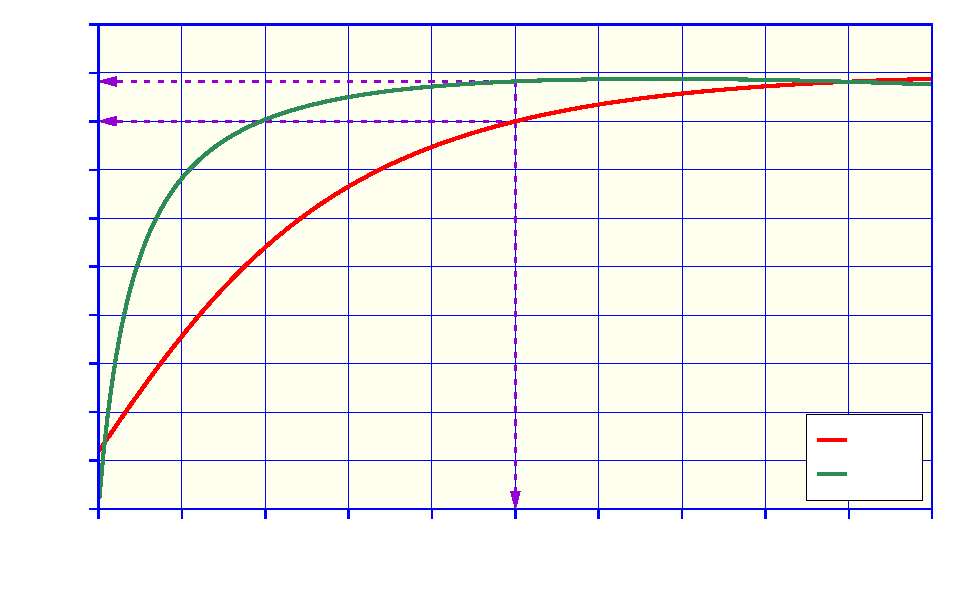
\includegraphics{Cap-Motors-Induccio-Ex6-2}}%
    \gplfronttext
  \end{picture}%
\endgroup

	\end{center}

\end{exemple}
	
\subsubsection{Tensió reduïda i càrrega nominal -- Solució aproximada}\index{motors d'inducció!tensió reduïda}

La potència mecànica que subministra un motor ve determinada per la potència que li demana la càrrega que arrossega, i per tant, si la tensió disminueix per sota del seu valor nominal, el corrent tendeix a augmentar per tal de mantenir la potència demandada, i el lliscament augmenta (és a dir, la velocitat es redueix).

Si en l'equació \eqref{eq:Pm-U1-Yeq} fixem $P\ped{m}$ al seu valor nominal, i $U_1$ al valor reduït existent, la podrem resoldre obtenint el valor de $s$ corresponent  a aquesta situació. Un cop tenim $s$, podem trobar la intensitat del motor $I_1$ utilitzant les equacions \eqref{eq:mot-Zmot} i \eqref{eq:mot-I1}. És clar que també podem trobar qualsevol altre valor del motor, com  ara el factor de potència o el rendiment, utilitzant les equacions pertinents.

Evidentment, aquest mètode de càlcul només és aproximat, ja que no té en compte la corba parell-velocitat de la càrrega arrossegada pel motor. En realitat, tal com es veurà en l'apartat següent, en general la potència mecànica no es manté constant.

\begin{exemple}[Motor alimentat a tensió reduïda -- Solució aproximada]
	\addcontentsxms{Motor alimentat a tensió reduïda -- Solució aproximada}
	Partim del mateix motor utilitzat en l'exemple \vref{ex:mot}, però alimentat al \qty{80}{\%} de la tensió nominal. Es tracta de trobar el corrent, el factor de potència i el rendiment del motor en aquestes condicions.
	
	La potència mecànica nominal, calculada  en l'exemple \ref{ex:mot}, val: \[
	P\ped{m,n} = \qty{9052,8}{W}
	\]
	
	El \qty{80}{\%} de la tensió fase--neutre nominal, calculada  en l'exemple \ref{ex:mot}, val:
	\[
	U_1 = 0{,}8\times\qty{219,393}{V} = \qty{175,514}{V}
	\]
	
	Els valors de $\cmplx{Z}_0$ i  $\cmplx{Z}\ped{Th}$, els quals no depenen del lliscament, també s'han calculat en  l'exemple \ref{ex:mot}, i valen:
	\begin{align*}
	\cmplx{Z}_0 &=  \complexqty{4,390+j39,512}{\ohm} \\[1ex]
	\cmplx{Z}\ped{Th} &= \complexqty{0,470+j1,448}{\ohm} 
	\end{align*}
	
	A continuació cal substituir aquests valors en l'equació \eqref{eq:Pm-U1-Yeq} i resoldre-la. Aquesta equació és clarament no lineal, i per tal de resoldre-la cal utilitzar programes de càlcul o mètodes numèrics, com ara els explicats en l'apèndix \ref{sec:func-no-lin}. La solució és:
	\[
	s = 0{,}097
	\]
	
	Utilitzant les equacions \eqref{eq:mot-Zmot} i \eqref{eq:mot-I1} amb $s  = 0{,}097$, trobem el corrent del motor:
	\begin{align*}
	\cmplx{Z}\ped{mot}(0{,}097) &=  \complexqty{6,324+j3,565}{\ohm} \\[1ex]
	I_1(0{,}097) &= \frac{\qty{175,514}{V}}{|\complexqty{6,324+j3,565}{\ohm}|} = \qty{24,2}{A}
	\end{align*}
	
	La relació entre aquest  corrent i el corrent nominal a tensió i potència nominals, calculat en l'exemple \ref{ex:mot}, és:
	\[
	\frac{I_1(0{,}097)}{I\ped{1,n}} = \frac{\qty{24,2}{A}}{\qty{17,7}{A}} = 1{,}4
	\]
	
	Finalment, utilitzant les equacions  \eqref{eq:cos-fi-mot} i \eqref{eq:mot-rendim} amb $s  = 0{,}097$, podem calcular els valors del factor de potència i del rendiment:
	\begin{align*}
	\cos\varphi(0{,}097) &=  0{,}871 \\
	\eta(0{,}097) &=  0{,}816
	\end{align*}
	
	Aquests dos valors són similars als valors calculats a tensió nominal en  l'exemple \ref{ex:mot}: 0,887 i 0,876 respectivament.
	
	Representem a continuació dues gràfiques. En la primera s'hi pot veure  l'evolució del lliscament $s$ i del corrent $I_1$ respecte de la relació entre la tensió aplicada i la tensió nominal $U_1/U\ped{n}$, indicant-hi els valors del lliscament i de la intensitat calculats anteriorment:
	\begin{center}
		% GNUPLOT: LaTeX picture with Postscript
\begingroup
  \makeatletter
  \providecommand\color[2][]{%
    \GenericError{(gnuplot) \space\space\space\@spaces}{%
      Package color not loaded in conjunction with
      terminal option `colourtext'%
    }{See the gnuplot documentation for explanation.%
    }{Either use 'blacktext' in gnuplot or load the package
      color.sty in LaTeX.}%
    \renewcommand\color[2][]{}%
  }%
  \providecommand\includegraphics[2][]{%
    \GenericError{(gnuplot) \space\space\space\@spaces}{%
      Package graphicx or graphics not loaded%
    }{See the gnuplot documentation for explanation.%
    }{The gnuplot epslatex terminal needs graphicx.sty or graphics.sty.}%
    \renewcommand\includegraphics[2][]{}%
  }%
  \providecommand\rotatebox[2]{#2}%
  \@ifundefined{ifGPcolor}{%
    \newif\ifGPcolor
    \GPcolortrue
  }{}%
  \@ifundefined{ifGPblacktext}{%
    \newif\ifGPblacktext
    \GPblacktexttrue
  }{}%
  % define a \g@addto@macro without @ in the name:
  \let\gplgaddtomacro\g@addto@macro
  % define empty templates for all commands taking text:
  \gdef\gplbacktext{}%
  \gdef\gplfronttext{}%
  \makeatother
  \ifGPblacktext
    % no textcolor at all
    \def\colorrgb#1{}%
    \def\colorgray#1{}%
  \else
    % gray or color?
    \ifGPcolor
      \def\colorrgb#1{\color[rgb]{#1}}%
      \def\colorgray#1{\color[gray]{#1}}%
      \expandafter\def\csname LTw\endcsname{\color{white}}%
      \expandafter\def\csname LTb\endcsname{\color{black}}%
      \expandafter\def\csname LTa\endcsname{\color{black}}%
      \expandafter\def\csname LT0\endcsname{\color[rgb]{1,0,0}}%
      \expandafter\def\csname LT1\endcsname{\color[rgb]{0,1,0}}%
      \expandafter\def\csname LT2\endcsname{\color[rgb]{0,0,1}}%
      \expandafter\def\csname LT3\endcsname{\color[rgb]{1,0,1}}%
      \expandafter\def\csname LT4\endcsname{\color[rgb]{0,1,1}}%
      \expandafter\def\csname LT5\endcsname{\color[rgb]{1,1,0}}%
      \expandafter\def\csname LT6\endcsname{\color[rgb]{0,0,0}}%
      \expandafter\def\csname LT7\endcsname{\color[rgb]{1,0.3,0}}%
      \expandafter\def\csname LT8\endcsname{\color[rgb]{0.5,0.5,0.5}}%
    \else
      % gray
      \def\colorrgb#1{\color{black}}%
      \def\colorgray#1{\color[gray]{#1}}%
      \expandafter\def\csname LTw\endcsname{\color{white}}%
      \expandafter\def\csname LTb\endcsname{\color{black}}%
      \expandafter\def\csname LTa\endcsname{\color{black}}%
      \expandafter\def\csname LT0\endcsname{\color{black}}%
      \expandafter\def\csname LT1\endcsname{\color{black}}%
      \expandafter\def\csname LT2\endcsname{\color{black}}%
      \expandafter\def\csname LT3\endcsname{\color{black}}%
      \expandafter\def\csname LT4\endcsname{\color{black}}%
      \expandafter\def\csname LT5\endcsname{\color{black}}%
      \expandafter\def\csname LT6\endcsname{\color{black}}%
      \expandafter\def\csname LT7\endcsname{\color{black}}%
      \expandafter\def\csname LT8\endcsname{\color{black}}%
    \fi
  \fi
    \setlength{\unitlength}{0.0500bp}%
    \ifx\gptboxheight\undefined%
      \newlength{\gptboxheight}%
      \newlength{\gptboxwidth}%
      \newsavebox{\gptboxtext}%
    \fi%
    \setlength{\fboxrule}{0.5pt}%
    \setlength{\fboxsep}{1pt}%
\begin{picture}(9340.00,5660.00)%
    \gplgaddtomacro\gplbacktext{%
      \colorrgb{0.00,0.00,0.00}%%
      \put(921,787){\makebox(0,0)[r]{\strut{} 0,00}}%
      \colorrgb{0.00,0.00,0.00}%%
      \put(921,1452){\makebox(0,0)[r]{\strut{} 0,02}}%
      \colorrgb{0.00,0.00,0.00}%%
      \put(921,2116){\makebox(0,0)[r]{\strut{} 0,04}}%
      \colorrgb{0.00,0.00,0.00}%%
      \put(921,2781){\makebox(0,0)[r]{\strut{} 0,06}}%
      \colorrgb{0.00,0.00,0.00}%%
      \put(921,3446){\makebox(0,0)[r]{\strut{} 0,08}}%
      \colorrgb{0.00,0.00,0.00}%%
      \put(921,4111){\makebox(0,0)[r]{\strut{} 0,10}}%
      \colorrgb{0.00,0.00,0.00}%%
      \put(921,4775){\makebox(0,0)[r]{\strut{} 0,12}}%
      \colorrgb{0.00,0.00,0.00}%%
      \put(921,5440){\makebox(0,0)[r]{\strut{} 0,14}}%
      \colorrgb{0.00,0.00,0.00}%%
      \put(1105,481){\makebox(0,0){\strut{} 0,75}}%
      \colorrgb{0.00,0.00,0.00}%%
      \put(2535,481){\makebox(0,0){\strut{} 0,80}}%
      \colorrgb{0.00,0.00,0.00}%%
      \put(3966,481){\makebox(0,0){\strut{} 0,85}}%
      \colorrgb{0.00,0.00,0.00}%%
      \put(5396,481){\makebox(0,0){\strut{} 0,90}}%
      \colorrgb{0.00,0.00,0.00}%%
      \put(6827,481){\makebox(0,0){\strut{} 0,95}}%
      \colorrgb{0.00,0.00,0.00}%%
      \put(8257,481){\makebox(0,0){\strut{} 1,00}}%
      \colorrgb{0.00,0.00,0.00}%%
      \put(8441,787){\makebox(0,0)[l]{\strut{} 16}}%
      \colorrgb{0.00,0.00,0.00}%%
      \put(8441,1452){\makebox(0,0)[l]{\strut{} 18}}%
      \colorrgb{0.00,0.00,0.00}%%
      \put(8441,2116){\makebox(0,0)[l]{\strut{} 20}}%
      \colorrgb{0.00,0.00,0.00}%%
      \put(8441,2781){\makebox(0,0)[l]{\strut{} 22}}%
      \colorrgb{0.00,0.00,0.00}%%
      \put(8441,3446){\makebox(0,0)[l]{\strut{} 24}}%
      \colorrgb{0.00,0.00,0.00}%%
      \put(8441,4111){\makebox(0,0)[l]{\strut{} 26}}%
      \colorrgb{0.00,0.00,0.00}%%
      \put(8441,4775){\makebox(0,0)[l]{\strut{} 28}}%
      \colorrgb{0.00,0.00,0.00}%%
      \put(8441,5440){\makebox(0,0)[l]{\strut{} 30}}%
    }%
    \gplgaddtomacro\gplfronttext{%
      \csname LTb\endcsname%%
      \put(291,3113){\makebox(0,0){\strut{}$s$}}%
      \csname LTb\endcsname%%
      \put(8938,3113){\rotatebox{-270}{\makebox(0,0){\strut{}$I_1\, / \,\si{A}$}}}%
      \csname LTb\endcsname%%
      \put(4681,153){\makebox(0,0){\strut{}$U_1/U\ped{n}$}}%
      \csname LTb\endcsname%%
      \put(4681,5331){\makebox(0,0){\strut{}}}%
      \csname LTb\endcsname%%
      \put(4681,5440){\makebox(0,0){\strut{}}}%
      \csname LTb\endcsname%%
      \put(7801,5189){\makebox(0,0){\strut{}}}%
      \csname LTb\endcsname%%
      \put(7918,5107){\makebox(0,0)[l]{\strut{}$s$}}%
      \csname LTb\endcsname%%
      \put(7918,4779){\makebox(0,0)[l]{\strut{}$I_1$}}%
      \csname LTb\endcsname%%
      \put(2450,1202){\rotatebox{-270}{\makebox(0,0){$\scriptstyle\num{0,8}$}}}%
      \csname LTb\endcsname%%
      \put(1563,3895){\makebox(0,0){$\scriptstyle\num{0,097}$}}%
      \csname LTb\endcsname%%
      \put(7542,3612){\makebox(0,0){$\scriptstyle\SI{24,2}{A}$}}%
    }%
    \gplbacktext
    \put(0,0){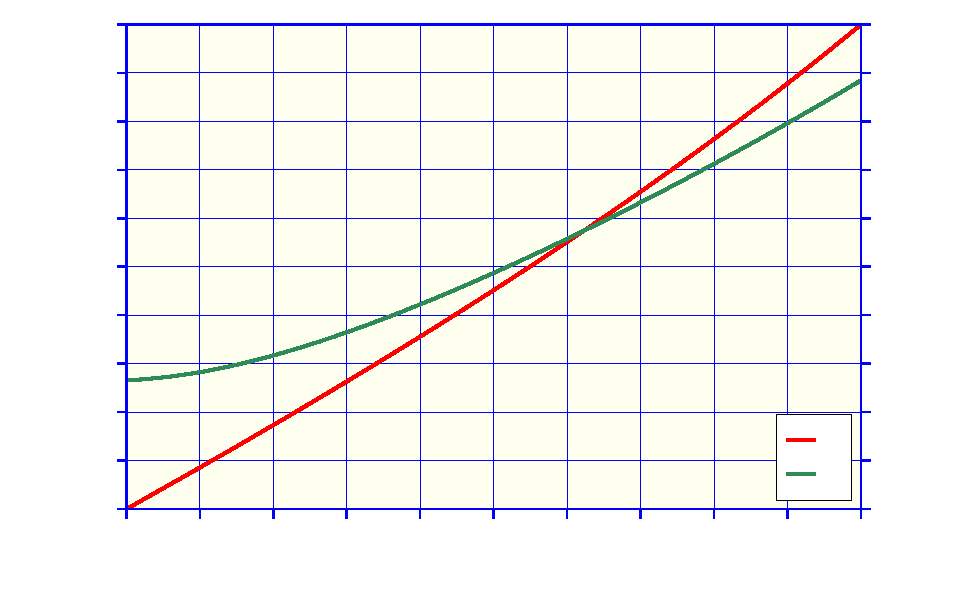
\includegraphics{Cap-Motors-Induccio-Ex7-1}}%
    \gplfronttext
  \end{picture}%
\endgroup

	\end{center}

	I en la segona s'hi pot veure l'evolució del factor de potència $\cos\varphi$ i del rendiment $\eta$ respecte de la relació entre la tensió aplicada i la tensió nominal $U_1/U\ped{n}$, indicant-hi també  els valors del factor de potència i del rendiment calculats anteriorment:
	\begin{center}
		% GNUPLOT: LaTeX picture with Postscript
\begingroup
  \makeatletter
  \providecommand\color[2][]{%
    \GenericError{(gnuplot) \space\space\space\@spaces}{%
      Package color not loaded in conjunction with
      terminal option `colourtext'%
    }{See the gnuplot documentation for explanation.%
    }{Either use 'blacktext' in gnuplot or load the package
      color.sty in LaTeX.}%
    \renewcommand\color[2][]{}%
  }%
  \providecommand\includegraphics[2][]{%
    \GenericError{(gnuplot) \space\space\space\@spaces}{%
      Package graphicx or graphics not loaded%
    }{See the gnuplot documentation for explanation.%
    }{The gnuplot epslatex terminal needs graphicx.sty or graphics.sty.}%
    \renewcommand\includegraphics[2][]{}%
  }%
  \providecommand\rotatebox[2]{#2}%
  \@ifundefined{ifGPcolor}{%
    \newif\ifGPcolor
    \GPcolortrue
  }{}%
  \@ifundefined{ifGPblacktext}{%
    \newif\ifGPblacktext
    \GPblacktexttrue
  }{}%
  % define a \g@addto@macro without @ in the name:
  \let\gplgaddtomacro\g@addto@macro
  % define empty templates for all commands taking text:
  \gdef\gplbacktext{}%
  \gdef\gplfronttext{}%
  \makeatother
  \ifGPblacktext
    % no textcolor at all
    \def\colorrgb#1{}%
    \def\colorgray#1{}%
  \else
    % gray or color?
    \ifGPcolor
      \def\colorrgb#1{\color[rgb]{#1}}%
      \def\colorgray#1{\color[gray]{#1}}%
      \expandafter\def\csname LTw\endcsname{\color{white}}%
      \expandafter\def\csname LTb\endcsname{\color{black}}%
      \expandafter\def\csname LTa\endcsname{\color{black}}%
      \expandafter\def\csname LT0\endcsname{\color[rgb]{1,0,0}}%
      \expandafter\def\csname LT1\endcsname{\color[rgb]{0,1,0}}%
      \expandafter\def\csname LT2\endcsname{\color[rgb]{0,0,1}}%
      \expandafter\def\csname LT3\endcsname{\color[rgb]{1,0,1}}%
      \expandafter\def\csname LT4\endcsname{\color[rgb]{0,1,1}}%
      \expandafter\def\csname LT5\endcsname{\color[rgb]{1,1,0}}%
      \expandafter\def\csname LT6\endcsname{\color[rgb]{0,0,0}}%
      \expandafter\def\csname LT7\endcsname{\color[rgb]{1,0.3,0}}%
      \expandafter\def\csname LT8\endcsname{\color[rgb]{0.5,0.5,0.5}}%
    \else
      % gray
      \def\colorrgb#1{\color{black}}%
      \def\colorgray#1{\color[gray]{#1}}%
      \expandafter\def\csname LTw\endcsname{\color{white}}%
      \expandafter\def\csname LTb\endcsname{\color{black}}%
      \expandafter\def\csname LTa\endcsname{\color{black}}%
      \expandafter\def\csname LT0\endcsname{\color{black}}%
      \expandafter\def\csname LT1\endcsname{\color{black}}%
      \expandafter\def\csname LT2\endcsname{\color{black}}%
      \expandafter\def\csname LT3\endcsname{\color{black}}%
      \expandafter\def\csname LT4\endcsname{\color{black}}%
      \expandafter\def\csname LT5\endcsname{\color{black}}%
      \expandafter\def\csname LT6\endcsname{\color{black}}%
      \expandafter\def\csname LT7\endcsname{\color{black}}%
      \expandafter\def\csname LT8\endcsname{\color{black}}%
    \fi
  \fi
    \setlength{\unitlength}{0.0500bp}%
    \ifx\gptboxheight\undefined%
      \newlength{\gptboxheight}%
      \newlength{\gptboxwidth}%
      \newsavebox{\gptboxtext}%
    \fi%
    \setlength{\fboxrule}{0.5pt}%
    \setlength{\fboxsep}{1pt}%
\begin{picture}(9340.00,5660.00)%
    \gplgaddtomacro\gplbacktext{%
      \colorrgb{0.00,0.00,0.00}%%
      \put(849,787){\makebox(0,0)[r]{\strut{} 0,76}}%
      \colorrgb{0.00,0.00,0.00}%%
      \put(849,1452){\makebox(0,0)[r]{\strut{} 0,78}}%
      \colorrgb{0.00,0.00,0.00}%%
      \put(849,2116){\makebox(0,0)[r]{\strut{} 0,80}}%
      \colorrgb{0.00,0.00,0.00}%%
      \put(849,2781){\makebox(0,0)[r]{\strut{} 0,82}}%
      \colorrgb{0.00,0.00,0.00}%%
      \put(849,3446){\makebox(0,0)[r]{\strut{} 0,84}}%
      \colorrgb{0.00,0.00,0.00}%%
      \put(849,4111){\makebox(0,0)[r]{\strut{} 0,86}}%
      \colorrgb{0.00,0.00,0.00}%%
      \put(849,4775){\makebox(0,0)[r]{\strut{} 0,88}}%
      \colorrgb{0.00,0.00,0.00}%%
      \put(849,5440){\makebox(0,0)[r]{\strut{} 0,90}}%
      \colorrgb{0.00,0.00,0.00}%%
      \put(1033,481){\makebox(0,0){\strut{} 0,75}}%
      \colorrgb{0.00,0.00,0.00}%%
      \put(2614,481){\makebox(0,0){\strut{} 0,80}}%
      \colorrgb{0.00,0.00,0.00}%%
      \put(4195,481){\makebox(0,0){\strut{} 0,85}}%
      \colorrgb{0.00,0.00,0.00}%%
      \put(5777,481){\makebox(0,0){\strut{} 0,90}}%
      \colorrgb{0.00,0.00,0.00}%%
      \put(7358,481){\makebox(0,0){\strut{} 0,95}}%
      \colorrgb{0.00,0.00,0.00}%%
      \put(8939,481){\makebox(0,0){\strut{} 1,00}}%
    }%
    \gplgaddtomacro\gplfronttext{%
      \csname LTb\endcsname%%
      \put(255,3113){\rotatebox{-270}{\makebox(0,0){\strut{}$\cos\varphi, \quad \eta$}}}%
      \csname LTb\endcsname%%
      \put(8993,3113){\rotatebox{-270}{\makebox(0,0){\strut{}}}}%
      \csname LTb\endcsname%%
      \put(4986,153){\makebox(0,0){\strut{}$U_1/U\ped{n}$}}%
      \csname LTb\endcsname%%
      \put(4986,5331){\makebox(0,0){\strut{}}}%
      \csname LTb\endcsname%%
      \put(4986,5440){\makebox(0,0){\strut{}}}%
      \csname LTb\endcsname%%
      \put(8289,1530){\makebox(0,0){\strut{}}}%
      \csname LTb\endcsname%%
      \put(8212,1448){\makebox(0,0)[l]{\strut{}$\cos\varphi$}}%
      \csname LTb\endcsname%%
      \put(8212,1120){\makebox(0,0)[l]{\strut{}$\eta$}}%
      \csname LTb\endcsname%%
      \put(2488,1119){\rotatebox{-270}{\makebox(0,0){$\scriptstyle\num{0,8}$}}}%
      \csname LTb\endcsname%%
      \put(1824,4576){\makebox(0,0){$\scriptstyle\num{0,871}$}}%
      \csname LTb\endcsname%%
      \put(1824,2515){\makebox(0,0){$\scriptstyle\num{0,816}$}}%
    }%
    \gplbacktext
    \put(0,0){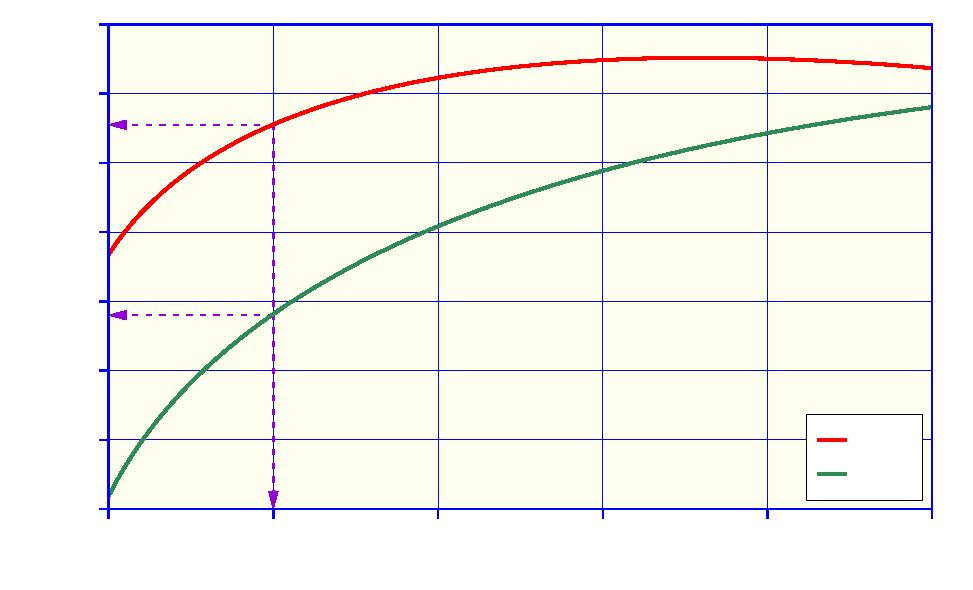
\includegraphics{Cap-Motors-Induccio-Ex7-2}}%
    \gplfronttext
  \end{picture}%
\endgroup

	\end{center}	
\end{exemple}

\subsubsection{Tensió reduïda i càrrega nominal -- Solució exacta}\index{motors d'inducció!tensió reduïda}

Tal com s'ha dit abans, el mètode de càlcul de l'apartat anterior només és aproximat, ja que no té en compte la corba parell-velocitat de la càrrega arrossegada pel motor. En realitat, en modificar-se la corba parell-velocitat del motor a causa de la tensió reduïda, el punt de tall d'aquesta corba amb la corba de la càrrega varia. Donat que el parell i la velocitat estan relacionats amb la potència segons l'equació  \eqref{eq:T-P-w}, en general i depenent de la forma de la corba parell-velocitat de la càrrega, el que passa és que el parell es manté,  disminueix o augmenta, fent que la potència també variï.

La forma de la corba parell-velocitat de les càrregues varia depenent de la seva naturalesa. En general podem distingir:
\begin{itemize}
	\item  \textbf{Relació constant}. El parell es manté constant per a qualsevol velocitat. Un exemple típic són els elevadors de corró.
	
	\item  \textbf{Relació lineal}. El parell varia lineament amb la velocitat. Un exemple típic són les bombes helicoidals de desplaçament positiu.
	
	\item  \textbf{Relació quadràtica}. El parell varia de forma  quadràtica  amb la velocitat. Un exemple típic són les bombes centrífugues i els ventiladors.
	
	\item  \textbf{Altres relacions}. És possible altres tipus de relacions, com ara inversa -- el parell disminueix amb la velocitat, o polinòmica -- el parell depèn de la velocitat segons una corba polinòmica de grau superior a 2.
\end{itemize}

No és  usual per a una càrrega (bomba ventilador, etc.) de disposar de l'expressió matemàtica que lliga el parell amb la velocitat; en aquest cas a partir de les gràfiques publicades sempre es pot fer un ajust, per exemple pel mètode dels mínims quadrats, i obtenir una expressió matemàtica. En el cas que tinguem una expressió matemàtica, prenent per exemple una relació quadràtica, serà del tipus:
\begin{equation}
	T\ped{load}(v) = a_0 v + a_1 v^2
\end{equation}

On $v$ pot ser directament la velocitat $n\ped{m}$ (en general expressada en r/min),  la relació entre la velocitat i la velocitat síncrona del motor $n\ped{m}/n\ped{m,sinc}$ o la relació entre la velocitat i la velocitat nominal de la càrrega $n\ped{m}/n\ped{m,n}$, la qual no serà en general igual a la velocitat síncrona del motor. Per tal de tenir l'expressió del parell respecte del lliscament,  seguint amb l'exemple de relació quadràtica, haurem d'utilitzar les transformacions següents:
\begin{equation}\label{eq:Tload-v-s}
	T\ped{load}(s) = \begin{cases}
		 a_0 n\ped{m,sinc}(1-s) + a_1 (n\ped{m,sinc}(1-s))^2,  & v=n\ped{m}  \\[2ex]
		a_0 (1-s) + a_1 (1-s)^2, &   
		v =\dfrac{n\ped{m}}{n\ped{m,sinc}} \\[2ex]
		 a_0 \dfrac{n\ped{m,sinc}}{n\ped{m,n}}(1-s) + a_1 \left(\dfrac{n\ped{m,sinc}}{n\ped{m,n}}(1-s)\right)^2, &    v = \dfrac{n\ped{m}}{n\ped{m,n}}
	\end{cases}
\end{equation}


Per tal de trobar el punt de tall, o de funcionament, de les corbes parell-velocitat del motor i de la càrrega per a una tensió d'alimentació donada, només cal establir l'igualat de l'expressió de $T\ped{load}(s)$ amb la de $T\ped{m}(s)$ segons l'equació \eqref{eq:Tm-U1-Yeq}, i resoldre-la per tal de trobar el lliscament $s\ped{fun}$ corresponent:
\begin{equation}\label{eq:Tload-U1-Yeq}
	T\ped{load}(s) = \frac{3 R_2 U_1^2}{s\omega\ped{m,sinc}}  \left( \frac{Z_0}{\big|R_1 + \ju X_1 + \cmplx{Z}_0\big| \left|\cmplx{Z}\ped{Th} + \dfrac{R_2}{s} + \ju X_2\right|} \right)^2 \quad\Rightarrow \quad s=s\ped{fun}
\end{equation}

\begin{exemple}[Motor alimentat a tensió reduïda -- Solució exacta]\label{ex:mot-tens-redu}
	\addcontentsxms{Motor alimentat a tensió reduïda -- Solució exacta}
	Partim del mateix motor utilitzat en l'exemple \vref{ex:mot} en dos casos: alimentat al \qty{100}{\%} i al \qty{80}{\%} de la tensió nominal. El motor arrossega un ventilador amb: $T\ped{load}(v) /{\scriptstyle \unit{N.m}} = 3{,}2 v + 58{,}9 v^2$, on $v = n\ped{m}/n\ped{m,sinc}$. Es tracta de trobar les característiques de funcionament del motor.
	
	El \qty{100}{\%} i \qty{80}{\%} de la tensió fase--neutre nominal, calculada  en l'exemple \ref{ex:mot}, val:
	\begin{align*}
		U_{1,\qty{100}{\%}} &= \qty{219,393}{V} \\
		U_{1,\qty{80}{\%}} &= 0{,}8\times\qty{219,393}{V} = \qty{175,514}{V}
	\end{align*}

	Els valors de $\omega\ped{m,sinc}$, $\cmplx{Z}_0$ i  $\cmplx{Z}\ped{Th}$, els quals no depenen del lliscament, també s'han calculat en  l'exemple \ref{ex:mot}, i valen:
	\vspace{-2mm}
	\begin{align*}
		\omega\ped{m,sinc} &=  \qty{157,080}{rad/s} \\
		\cmplx{Z}_0 &=  \complexqty{4,390+j39,512}{\ohm} \\
		\cmplx{Z}\ped{Th} &= \complexqty{0,470+j1,448}{\ohm} 
	\end{align*}
	
	L'equació de la corba parell-velocitat en newton metre, expressada en funció del lliscament $s$ és, tenint en compte l'equació \eqref{eq:Tload-v-s}:
	\[
		T\ped{load}(s) = 3{,}2 (1-s) + 58{,}9 (1-s)^2
	\]

	A continuació cal substituir aquests valors en l'equació \eqref{eq:Tload-U1-Yeq} i resoldre-la. Aquesta equació és clarament no lineal, i per tal de resoldre-la cal utilitzar programes de càlcul o mètodes numèrics, com ara els explicats en l'apèndix \ref{sec:func-no-lin}. Les solucions, per a $U_1=U_{1,\qty{100}{\%}}$ i $U_1=U_{1,\qty{80}{\%}}$, són:
	\begin{align*}
		s_{\qty{100}{\%}} = 0{,}046 \\
	 	s_{\qty{80}{\%}}= 0{,}075
	\end{align*}	
	
	Aquests lliscaments corresponen a les velocitats següents:
	\begin{align*}
		n\ped{\qty{100}{\%}} &= (1-\num{0,046})\times \qty{1500}{r/min} = \qty{1431}{r/min} \\
		n\ped{\qty{80}{\%}} &= (1-\num{0,075})\times \qty{1500}{r/min} = \qty{1387,5}{r/min}
	\end{align*}
	
	Utilitzant les equacions \eqref{eq:mot-Zmot} i \eqref{eq:mot-I1} podem calcular el valor del corrent nominal, i utilitzant les equacions \eqref{eq:Tm-U1-Yeq}, \eqref{eq:cos-fi-mot} i \eqref{eq:mot-rendim} podem calcular els valors del parell mecànic, del factor de potència i del rendiment. Amb $U_1 = U_{1,\qty{100}{\%}}$  i $s = s_{\qty{100}{\%}}$, obtenim:
	\begin{align*}
		I_{1,\qty{100}{\%}} &= \qty{16,6}{A} \\
		T\ped{m,\qty{100}{\%}} &=  \qty{56,6}{N.m} \\
		\cos\varphi_{\qty{100}{\%}} &=  0{,}884 \\
		\eta_{\qty{100}{\%}} &=  0{,}880
	\end{align*}
	
	Igualment, amb $U_1 = U_{1,\qty{80}{\%}}$ i $s = s_{\qty{80}{\%}}$, obtenim:
	\pagebreak
	\begin{align*}
		I_{1,\qty{80}{\%}} &= \qty{19,6}{A} \\
		T\ped{m,\qty{80}{\%}} &=  \qty{53,4}{N.m} \\
		\cos\varphi_{\qty{80}{\%}} &=  0{,}887 \\
		\eta_{\qty{80}{\%}} &=  0{,}847
	\end{align*}

	Utilitzant les equacions \eqref{eq:z-mot-arr} i \eqref{eq:I1-mot-arr} podem calcular el corrent d'arrencada del motor, i utilitzant l'equació \eqref{eq:Tm-U1-Yeq}, amb $s=1$, podem calcular els valors del parell mecànic d'arrencada. Amb $U_1 = U_{1,\qty{100}{\%}}$   obtenim:
	\vspace{-2mm}
	\begin{align*}
		I\ped{arr,\qty{100}{\%}} &=  \qty{74,9}{A} \\
		T\ped{m,arr,\qty{100}{\%}} &=  \qty{62,8}{N.m} 
	\end{align*}
	
	Igualment, amb $U_1 = U_{1,\qty{80}{\%}}$ obtenim:
	\vspace{-2mm}
	\begin{align*}
		I\ped{arr,\qty{80}{\%}} &=  \qty{59,9}{A} \\
		T\ped{m,arr,\qty{80}{\%}} &=  \qty{40,2}{N.m} 
	\end{align*}
	
	Es pot comprovar que es compleix: $I\ped{arr,\qty{80}{\%}} / I\ped{arr,\qty{100}{\%}} = 0{,}8$ i $T\ped{m,arr,\qty{80}{\%}} / T\ped{m,arr,\qty{100}{\%}} = 0{,}8^2 = 0{,}64$.
		
 	Representem ara la gràfica de l'evolució dels parells $T\ped{load}$,  $T\ped{m,\qty{100}{\%}}$,  $T\ped{m,\qty{80}{\%}}$, i dels	corrents I\ped{1,\qty{100}{\%}} i I\ped{1,\qty{80}{\%}} respecte de la velocitat $n\ped{m}$:	
    \begin{center}
		\fontsize{10pt}{11pt}\selectfont
		% GNUPLOT: LaTeX picture with Postscript
\begingroup
  \makeatletter
  \providecommand\color[2][]{%
    \GenericError{(gnuplot) \space\space\space\@spaces}{%
      Package color not loaded in conjunction with
      terminal option `colourtext'%
    }{See the gnuplot documentation for explanation.%
    }{Either use 'blacktext' in gnuplot or load the package
      color.sty in LaTeX.}%
    \renewcommand\color[2][]{}%
  }%
  \providecommand\includegraphics[2][]{%
    \GenericError{(gnuplot) \space\space\space\@spaces}{%
      Package graphicx or graphics not loaded%
    }{See the gnuplot documentation for explanation.%
    }{The gnuplot epslatex terminal needs graphicx.sty or graphics.sty.}%
    \renewcommand\includegraphics[2][]{}%
  }%
  \providecommand\rotatebox[2]{#2}%
  \@ifundefined{ifGPcolor}{%
    \newif\ifGPcolor
    \GPcolortrue
  }{}%
  \@ifundefined{ifGPblacktext}{%
    \newif\ifGPblacktext
    \GPblacktexttrue
  }{}%
  % define a \g@addto@macro without @ in the name:
  \let\gplgaddtomacro\g@addto@macro
  % define empty templates for all commands taking text:
  \gdef\gplbacktext{}%
  \gdef\gplfronttext{}%
  \makeatother
  \ifGPblacktext
    % no textcolor at all
    \def\colorrgb#1{}%
    \def\colorgray#1{}%
  \else
    % gray or color?
    \ifGPcolor
      \def\colorrgb#1{\color[rgb]{#1}}%
      \def\colorgray#1{\color[gray]{#1}}%
      \expandafter\def\csname LTw\endcsname{\color{white}}%
      \expandafter\def\csname LTb\endcsname{\color{black}}%
      \expandafter\def\csname LTa\endcsname{\color{black}}%
      \expandafter\def\csname LT0\endcsname{\color[rgb]{1,0,0}}%
      \expandafter\def\csname LT1\endcsname{\color[rgb]{0,1,0}}%
      \expandafter\def\csname LT2\endcsname{\color[rgb]{0,0,1}}%
      \expandafter\def\csname LT3\endcsname{\color[rgb]{1,0,1}}%
      \expandafter\def\csname LT4\endcsname{\color[rgb]{0,1,1}}%
      \expandafter\def\csname LT5\endcsname{\color[rgb]{1,1,0}}%
      \expandafter\def\csname LT6\endcsname{\color[rgb]{0,0,0}}%
      \expandafter\def\csname LT7\endcsname{\color[rgb]{1,0.3,0}}%
      \expandafter\def\csname LT8\endcsname{\color[rgb]{0.5,0.5,0.5}}%
    \else
      % gray
      \def\colorrgb#1{\color{black}}%
      \def\colorgray#1{\color[gray]{#1}}%
      \expandafter\def\csname LTw\endcsname{\color{white}}%
      \expandafter\def\csname LTb\endcsname{\color{black}}%
      \expandafter\def\csname LTa\endcsname{\color{black}}%
      \expandafter\def\csname LT0\endcsname{\color{black}}%
      \expandafter\def\csname LT1\endcsname{\color{black}}%
      \expandafter\def\csname LT2\endcsname{\color{black}}%
      \expandafter\def\csname LT3\endcsname{\color{black}}%
      \expandafter\def\csname LT4\endcsname{\color{black}}%
      \expandafter\def\csname LT5\endcsname{\color{black}}%
      \expandafter\def\csname LT6\endcsname{\color{black}}%
      \expandafter\def\csname LT7\endcsname{\color{black}}%
      \expandafter\def\csname LT8\endcsname{\color{black}}%
    \fi
  \fi
    \setlength{\unitlength}{0.0500bp}%
    \ifx\gptboxheight\undefined%
      \newlength{\gptboxheight}%
      \newlength{\gptboxwidth}%
      \newsavebox{\gptboxtext}%
    \fi%
    \setlength{\fboxrule}{0.5pt}%
    \setlength{\fboxsep}{1pt}%
\begin{picture}(9340.00,5660.00)%
    \gplgaddtomacro\gplbacktext{%
      \colorrgb{0.00,0.00,0.00}%%
      \put(752,787){\makebox(0,0)[r]{\strut{} 0}}%
      \colorrgb{0.00,0.00,0.00}%%
      \put(752,1097){\makebox(0,0)[r]{\strut{} 10}}%
      \colorrgb{0.00,0.00,0.00}%%
      \put(752,1407){\makebox(0,0)[r]{\strut{} 20}}%
      \colorrgb{0.00,0.00,0.00}%%
      \put(752,1718){\makebox(0,0)[r]{\strut{} 30}}%
      \colorrgb{0.00,0.00,0.00}%%
      \put(752,2028){\makebox(0,0)[r]{\strut{} 40}}%
      \colorrgb{0.00,0.00,0.00}%%
      \put(752,2338){\makebox(0,0)[r]{\strut{} 50}}%
      \colorrgb{0.00,0.00,0.00}%%
      \put(752,2648){\makebox(0,0)[r]{\strut{} 60}}%
      \colorrgb{0.00,0.00,0.00}%%
      \put(752,2958){\makebox(0,0)[r]{\strut{} 70}}%
      \colorrgb{0.00,0.00,0.00}%%
      \put(752,3269){\makebox(0,0)[r]{\strut{} 80}}%
      \colorrgb{0.00,0.00,0.00}%%
      \put(752,3579){\makebox(0,0)[r]{\strut{} 90}}%
      \colorrgb{0.00,0.00,0.00}%%
      \put(752,3889){\makebox(0,0)[r]{\strut{} 100}}%
      \colorrgb{0.00,0.00,0.00}%%
      \put(752,4199){\makebox(0,0)[r]{\strut{} 110}}%
      \colorrgb{0.00,0.00,0.00}%%
      \put(752,4509){\makebox(0,0)[r]{\strut{} 120}}%
      \colorrgb{0.00,0.00,0.00}%%
      \put(752,4820){\makebox(0,0)[r]{\strut{} 130}}%
      \colorrgb{0.00,0.00,0.00}%%
      \put(752,5130){\makebox(0,0)[r]{\strut{} 140}}%
      \colorrgb{0.00,0.00,0.00}%%
      \put(752,5440){\makebox(0,0)[r]{\strut{} 150}}%
      \colorrgb{0.00,0.00,0.00}%%
      \put(936,481){\makebox(0,0){\strut{} 0}}%
      \colorrgb{0.00,0.00,0.00}%%
      \put(1424,481){\makebox(0,0){\strut{} 100}}%
      \colorrgb{0.00,0.00,0.00}%%
      \put(1912,481){\makebox(0,0){\strut{} 200}}%
      \colorrgb{0.00,0.00,0.00}%%
      \put(2400,481){\makebox(0,0){\strut{} 300}}%
      \colorrgb{0.00,0.00,0.00}%%
      \put(2888,481){\makebox(0,0){\strut{} 400}}%
      \colorrgb{0.00,0.00,0.00}%%
      \put(3376,481){\makebox(0,0){\strut{} 500}}%
      \colorrgb{0.00,0.00,0.00}%%
      \put(3864,481){\makebox(0,0){\strut{} 600}}%
      \colorrgb{0.00,0.00,0.00}%%
      \put(4352,481){\makebox(0,0){\strut{} 700}}%
      \colorrgb{0.00,0.00,0.00}%%
      \put(4841,481){\makebox(0,0){\strut{} 800}}%
      \colorrgb{0.00,0.00,0.00}%%
      \put(5329,481){\makebox(0,0){\strut{} 900}}%
      \colorrgb{0.00,0.00,0.00}%%
      \put(5817,481){\makebox(0,0){\strut{} 1000}}%
      \colorrgb{0.00,0.00,0.00}%%
      \put(6305,481){\makebox(0,0){\strut{} 1100}}%
      \colorrgb{0.00,0.00,0.00}%%
      \put(6793,481){\makebox(0,0){\strut{} 1200}}%
      \colorrgb{0.00,0.00,0.00}%%
      \put(7281,481){\makebox(0,0){\strut{} 1300}}%
      \colorrgb{0.00,0.00,0.00}%%
      \put(7769,481){\makebox(0,0){\strut{} 1400}}%
      \colorrgb{0.00,0.00,0.00}%%
      \put(8257,481){\makebox(0,0){\strut{} 1500}}%
      \colorrgb{0.00,0.00,0.00}%%
      \put(8441,787){\makebox(0,0)[l]{\strut{} 0}}%
      \colorrgb{0.00,0.00,0.00}%%
      \put(8441,1097){\makebox(0,0)[l]{\strut{} 5}}%
      \colorrgb{0.00,0.00,0.00}%%
      \put(8441,1407){\makebox(0,0)[l]{\strut{} 10}}%
      \colorrgb{0.00,0.00,0.00}%%
      \put(8441,1718){\makebox(0,0)[l]{\strut{} 15}}%
      \colorrgb{0.00,0.00,0.00}%%
      \put(8441,2028){\makebox(0,0)[l]{\strut{} 20}}%
      \colorrgb{0.00,0.00,0.00}%%
      \put(8441,2338){\makebox(0,0)[l]{\strut{} 25}}%
      \colorrgb{0.00,0.00,0.00}%%
      \put(8441,2648){\makebox(0,0)[l]{\strut{} 30}}%
      \colorrgb{0.00,0.00,0.00}%%
      \put(8441,2958){\makebox(0,0)[l]{\strut{} 35}}%
      \colorrgb{0.00,0.00,0.00}%%
      \put(8441,3269){\makebox(0,0)[l]{\strut{} 40}}%
      \colorrgb{0.00,0.00,0.00}%%
      \put(8441,3579){\makebox(0,0)[l]{\strut{} 45}}%
      \colorrgb{0.00,0.00,0.00}%%
      \put(8441,3889){\makebox(0,0)[l]{\strut{} 50}}%
      \colorrgb{0.00,0.00,0.00}%%
      \put(8441,4199){\makebox(0,0)[l]{\strut{} 55}}%
      \colorrgb{0.00,0.00,0.00}%%
      \put(8441,4509){\makebox(0,0)[l]{\strut{} 60}}%
      \colorrgb{0.00,0.00,0.00}%%
      \put(8441,4820){\makebox(0,0)[l]{\strut{} 65}}%
      \colorrgb{0.00,0.00,0.00}%%
      \put(8441,5130){\makebox(0,0)[l]{\strut{} 70}}%
      \colorrgb{0.00,0.00,0.00}%%
      \put(8441,5440){\makebox(0,0)[l]{\strut{} 75}}%
    }%
    \gplgaddtomacro\gplfronttext{%
      \csname LTb\endcsname%%
      \put(255,3113){\rotatebox{-270}{\makebox(0,0){\strut{}$T\ped{m}\, / \,\si{N.m}, \quad T\ped{load}\, / \,\si{N.m}$}}}%
      \csname LTb\endcsname%%
      \put(8938,3113){\rotatebox{-270}{\makebox(0,0){\strut{}$I_1\, / \,\si{A}$}}}%
      \csname LTb\endcsname%%
      \put(4596,153){\makebox(0,0){\strut{}$n\ped{m}\, / \,\si{r/min}$}}%
      \csname LTb\endcsname%%
      \put(4596,5331){\makebox(0,0){\strut{}}}%
      \csname LTb\endcsname%%
      \put(4596,5440){\makebox(0,0){\strut{}}}%
      \csname LTb\endcsname%%
      \put(1677,4245){\makebox(0,0){\strut{}}}%
      \csname LTb\endcsname%%
      \put(1478,4217){\makebox(0,0)[l]{\strut{}$T\ped{load}$}}%
      \csname LTb\endcsname%%
      \put(1478,3998){\makebox(0,0)[l]{\strut{}$T\ped{m,\SI{100}{\%}}$}}%
      \csname LTb\endcsname%%
      \put(1478,3779){\makebox(0,0)[l]{\strut{}$T\ped{m,\SI{80}{\%}}$}}%
      \csname LTb\endcsname%%
      \put(1478,3560){\makebox(0,0)[l]{\strut{}$I\ped{1,\SI{100}{\%}}$}}%
      \csname LTb\endcsname%%
      \put(1478,3341){\makebox(0,0)[l]{\strut{}$I\ped{1,\SI{80}{\%}}$}}%
    }%
    \gplbacktext
    \put(0,0){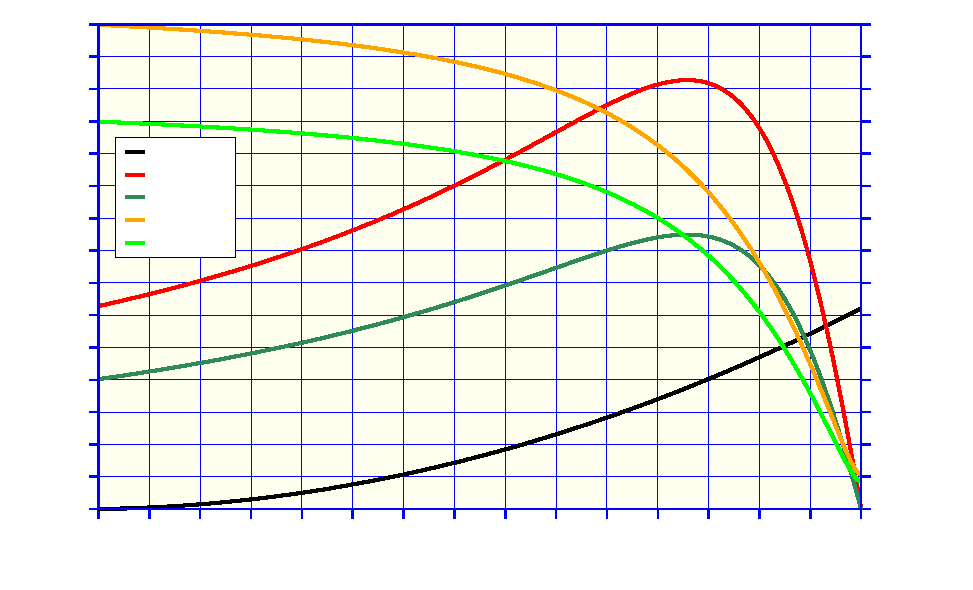
\includegraphics{Cap-Motors-Induccio-Ex8-1-1}}%
    \gplfronttext
  \end{picture}%
\endgroup

	\end{center}	

	\vspace{-2mm}
	A continuació es representa una zona ampliada de la gràfica anterior en el rang de velocitats compreses entre \qty{1200}{r/min} i  \qty{1500}{r/min}, indicant-hi els parells, corrents i velocitats calculades anteriorment:

	\begin{center}
		\fontsize{10pt}{11pt}\selectfont
		% GNUPLOT: LaTeX picture with Postscript
\begingroup
  \makeatletter
  \providecommand\color[2][]{%
    \GenericError{(gnuplot) \space\space\space\@spaces}{%
      Package color not loaded in conjunction with
      terminal option `colourtext'%
    }{See the gnuplot documentation for explanation.%
    }{Either use 'blacktext' in gnuplot or load the package
      color.sty in LaTeX.}%
    \renewcommand\color[2][]{}%
  }%
  \providecommand\includegraphics[2][]{%
    \GenericError{(gnuplot) \space\space\space\@spaces}{%
      Package graphicx or graphics not loaded%
    }{See the gnuplot documentation for explanation.%
    }{The gnuplot epslatex terminal needs graphicx.sty or graphics.sty.}%
    \renewcommand\includegraphics[2][]{}%
  }%
  \providecommand\rotatebox[2]{#2}%
  \@ifundefined{ifGPcolor}{%
    \newif\ifGPcolor
    \GPcolortrue
  }{}%
  \@ifundefined{ifGPblacktext}{%
    \newif\ifGPblacktext
    \GPblacktexttrue
  }{}%
  % define a \g@addto@macro without @ in the name:
  \let\gplgaddtomacro\g@addto@macro
  % define empty templates for all commands taking text:
  \gdef\gplbacktext{}%
  \gdef\gplfronttext{}%
  \makeatother
  \ifGPblacktext
    % no textcolor at all
    \def\colorrgb#1{}%
    \def\colorgray#1{}%
  \else
    % gray or color?
    \ifGPcolor
      \def\colorrgb#1{\color[rgb]{#1}}%
      \def\colorgray#1{\color[gray]{#1}}%
      \expandafter\def\csname LTw\endcsname{\color{white}}%
      \expandafter\def\csname LTb\endcsname{\color{black}}%
      \expandafter\def\csname LTa\endcsname{\color{black}}%
      \expandafter\def\csname LT0\endcsname{\color[rgb]{1,0,0}}%
      \expandafter\def\csname LT1\endcsname{\color[rgb]{0,1,0}}%
      \expandafter\def\csname LT2\endcsname{\color[rgb]{0,0,1}}%
      \expandafter\def\csname LT3\endcsname{\color[rgb]{1,0,1}}%
      \expandafter\def\csname LT4\endcsname{\color[rgb]{0,1,1}}%
      \expandafter\def\csname LT5\endcsname{\color[rgb]{1,1,0}}%
      \expandafter\def\csname LT6\endcsname{\color[rgb]{0,0,0}}%
      \expandafter\def\csname LT7\endcsname{\color[rgb]{1,0.3,0}}%
      \expandafter\def\csname LT8\endcsname{\color[rgb]{0.5,0.5,0.5}}%
    \else
      % gray
      \def\colorrgb#1{\color{black}}%
      \def\colorgray#1{\color[gray]{#1}}%
      \expandafter\def\csname LTw\endcsname{\color{white}}%
      \expandafter\def\csname LTb\endcsname{\color{black}}%
      \expandafter\def\csname LTa\endcsname{\color{black}}%
      \expandafter\def\csname LT0\endcsname{\color{black}}%
      \expandafter\def\csname LT1\endcsname{\color{black}}%
      \expandafter\def\csname LT2\endcsname{\color{black}}%
      \expandafter\def\csname LT3\endcsname{\color{black}}%
      \expandafter\def\csname LT4\endcsname{\color{black}}%
      \expandafter\def\csname LT5\endcsname{\color{black}}%
      \expandafter\def\csname LT6\endcsname{\color{black}}%
      \expandafter\def\csname LT7\endcsname{\color{black}}%
      \expandafter\def\csname LT8\endcsname{\color{black}}%
    \fi
  \fi
    \setlength{\unitlength}{0.0500bp}%
    \ifx\gptboxheight\undefined%
      \newlength{\gptboxheight}%
      \newlength{\gptboxwidth}%
      \newsavebox{\gptboxtext}%
    \fi%
    \setlength{\fboxrule}{0.5pt}%
    \setlength{\fboxsep}{1pt}%
\begin{picture}(9340.00,5660.00)%
    \gplgaddtomacro\gplbacktext{%
      \colorrgb{0.00,0.00,0.00}%%
      \put(655,787){\makebox(0,0)[r]{\strut{} 0}}%
      \colorrgb{0.00,0.00,0.00}%%
      \put(655,1304){\makebox(0,0)[r]{\strut{} 10}}%
      \colorrgb{0.00,0.00,0.00}%%
      \put(655,1821){\makebox(0,0)[r]{\strut{} 20}}%
      \colorrgb{0.00,0.00,0.00}%%
      \put(655,2338){\makebox(0,0)[r]{\strut{} 30}}%
      \colorrgb{0.00,0.00,0.00}%%
      \put(655,2855){\makebox(0,0)[r]{\strut{} 40}}%
      \colorrgb{0.00,0.00,0.00}%%
      \put(655,3372){\makebox(0,0)[r]{\strut{} 50}}%
      \colorrgb{0.00,0.00,0.00}%%
      \put(655,3889){\makebox(0,0)[r]{\strut{} 60}}%
      \colorrgb{0.00,0.00,0.00}%%
      \put(655,4406){\makebox(0,0)[r]{\strut{} 70}}%
      \colorrgb{0.00,0.00,0.00}%%
      \put(655,4923){\makebox(0,0)[r]{\strut{} 80}}%
      \colorrgb{0.00,0.00,0.00}%%
      \put(655,5440){\makebox(0,0)[r]{\strut{} 90}}%
      \colorrgb{0.00,0.00,0.00}%%
      \put(839,481){\makebox(0,0){\strut{} 1200}}%
      \colorrgb{0.00,0.00,0.00}%%
      \put(2075,481){\makebox(0,0){\strut{} 1250}}%
      \colorrgb{0.00,0.00,0.00}%%
      \put(3312,481){\makebox(0,0){\strut{} 1300}}%
      \colorrgb{0.00,0.00,0.00}%%
      \put(4548,481){\makebox(0,0){\strut{} 1350}}%
      \colorrgb{0.00,0.00,0.00}%%
      \put(5784,481){\makebox(0,0){\strut{} 1400}}%
      \colorrgb{0.00,0.00,0.00}%%
      \put(7021,481){\makebox(0,0){\strut{} 1450}}%
      \colorrgb{0.00,0.00,0.00}%%
      \put(8257,481){\makebox(0,0){\strut{} 1500}}%
      \colorrgb{0.00,0.00,0.00}%%
      \put(8441,787){\makebox(0,0)[l]{\strut{} 0}}%
      \colorrgb{0.00,0.00,0.00}%%
      \put(8441,1304){\makebox(0,0)[l]{\strut{} 5}}%
      \colorrgb{0.00,0.00,0.00}%%
      \put(8441,1821){\makebox(0,0)[l]{\strut{} 10}}%
      \colorrgb{0.00,0.00,0.00}%%
      \put(8441,2338){\makebox(0,0)[l]{\strut{} 15}}%
      \colorrgb{0.00,0.00,0.00}%%
      \put(8441,2855){\makebox(0,0)[l]{\strut{} 20}}%
      \colorrgb{0.00,0.00,0.00}%%
      \put(8441,3372){\makebox(0,0)[l]{\strut{} 25}}%
      \colorrgb{0.00,0.00,0.00}%%
      \put(8441,3889){\makebox(0,0)[l]{\strut{} 30}}%
      \colorrgb{0.00,0.00,0.00}%%
      \put(8441,4406){\makebox(0,0)[l]{\strut{} 35}}%
      \colorrgb{0.00,0.00,0.00}%%
      \put(8441,4923){\makebox(0,0)[l]{\strut{} 40}}%
      \colorrgb{0.00,0.00,0.00}%%
      \put(8441,5440){\makebox(0,0)[l]{\strut{} 45}}%
    }%
    \gplgaddtomacro\gplfronttext{%
      \csname LTb\endcsname%%
      \put(255,3113){\rotatebox{-270}{\makebox(0,0){\strut{}$T\ped{m}\, / \,\si{N.m}, \quad T\ped{load}\, / \,\si{N.m}$}}}%
      \csname LTb\endcsname%%
      \put(8938,3113){\rotatebox{-270}{\makebox(0,0){\strut{}$I_1\, / \,\si{A}$}}}%
      \csname LTb\endcsname%%
      \put(4548,153){\makebox(0,0){\strut{}$n\ped{m}\, / \,\si{r/min}$}}%
      \csname LTb\endcsname%%
      \put(4548,5331){\makebox(0,0){\strut{}}}%
      \csname LTb\endcsname%%
      \put(4548,5440){\makebox(0,0){\strut{}}}%
      \csname LTb\endcsname%%
      \put(1513,2079){\makebox(0,0){\strut{}}}%
      \csname LTb\endcsname%%
      \put(1314,1969){\makebox(0,0)[l]{\strut{}$T\ped{load}$}}%
      \csname LTb\endcsname%%
      \put(1314,1750){\makebox(0,0)[l]{\strut{}$T\ped{m,\SI{100}{\%}}$}}%
      \csname LTb\endcsname%%
      \put(1314,1531){\makebox(0,0)[l]{\strut{}$T\ped{m,\SI{80}{\%}}$}}%
      \csname LTb\endcsname%%
      \put(1314,1312){\makebox(0,0)[l]{\strut{}$I\ped{1,\SI{100}{\%}}$}}%
      \csname LTb\endcsname%%
      \put(1314,1093){\makebox(0,0)[l]{\strut{}$I\ped{1,\SI{80}{\%}}$}}%
      \csname LTb\endcsname%%
      \put(6452,1563){\rotatebox{-270}{\makebox(0,0){$\scriptstyle\SI{1431}{r/min}$}}}%
      \csname LTb\endcsname%%
      \put(5381,1563){\rotatebox{-270}{\makebox(0,0){$\scriptstyle\SI{1387,5}{r/min}$}}}%
      \csname LTb\endcsname%%
      \put(1581,3786){\makebox(0,0){$\scriptstyle\SI{56,6}{N.m}$}}%
      \csname LTb\endcsname%%
      \put(1581,3450){\makebox(0,0){$\scriptstyle\SI{53,4}{N.m}$}}%
      \csname LTb\endcsname%%
      \put(7762,2576){\makebox(0,0){$\scriptstyle\SI{16,6}{A}$}}%
      \csname LTb\endcsname%%
      \put(7762,2917){\makebox(0,0){$\scriptstyle\SI{19,6}{A}$}}%
    }%
    \gplbacktext
    \put(0,0){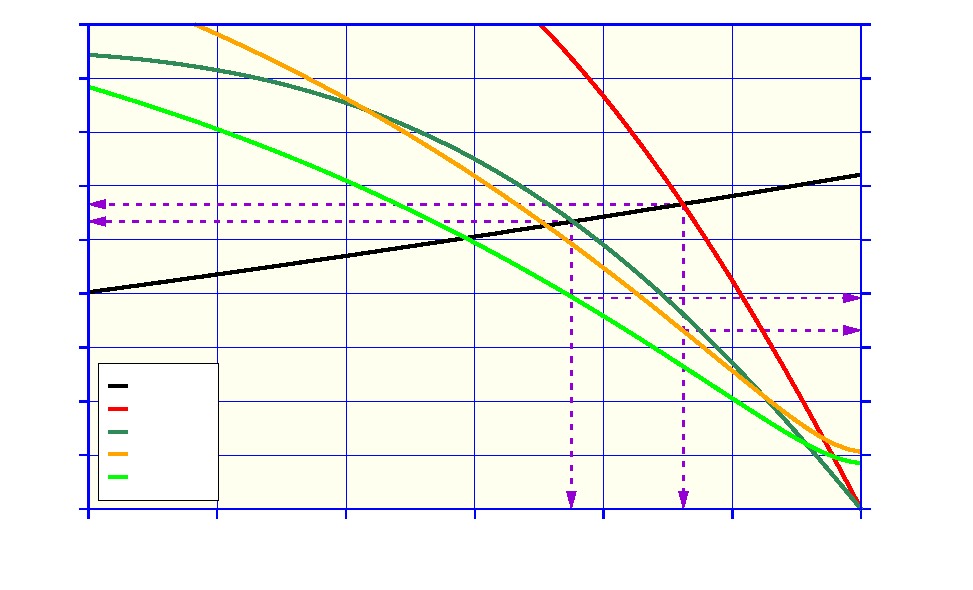
\includegraphics{Cap-Motors-Induccio-Ex8-1-2}}%
    \gplfronttext
  \end{picture}%
\endgroup

	\end{center}

	Representem a continuació dues gràfiques. En la primera s'hi pot veure  l'evolució del lliscament $s$ i del corrent $I_1$ respecte de la relació entre la tensió aplicada i la tensió nominal $U_1/U\ped{n}$:
	\begin{center}
		% GNUPLOT: LaTeX picture with Postscript
\begingroup
  \makeatletter
  \providecommand\color[2][]{%
    \GenericError{(gnuplot) \space\space\space\@spaces}{%
      Package color not loaded in conjunction with
      terminal option `colourtext'%
    }{See the gnuplot documentation for explanation.%
    }{Either use 'blacktext' in gnuplot or load the package
      color.sty in LaTeX.}%
    \renewcommand\color[2][]{}%
  }%
  \providecommand\includegraphics[2][]{%
    \GenericError{(gnuplot) \space\space\space\@spaces}{%
      Package graphicx or graphics not loaded%
    }{See the gnuplot documentation for explanation.%
    }{The gnuplot epslatex terminal needs graphicx.sty or graphics.sty.}%
    \renewcommand\includegraphics[2][]{}%
  }%
  \providecommand\rotatebox[2]{#2}%
  \@ifundefined{ifGPcolor}{%
    \newif\ifGPcolor
    \GPcolortrue
  }{}%
  \@ifundefined{ifGPblacktext}{%
    \newif\ifGPblacktext
    \GPblacktexttrue
  }{}%
  % define a \g@addto@macro without @ in the name:
  \let\gplgaddtomacro\g@addto@macro
  % define empty templates for all commands taking text:
  \gdef\gplbacktext{}%
  \gdef\gplfronttext{}%
  \makeatother
  \ifGPblacktext
    % no textcolor at all
    \def\colorrgb#1{}%
    \def\colorgray#1{}%
  \else
    % gray or color?
    \ifGPcolor
      \def\colorrgb#1{\color[rgb]{#1}}%
      \def\colorgray#1{\color[gray]{#1}}%
      \expandafter\def\csname LTw\endcsname{\color{white}}%
      \expandafter\def\csname LTb\endcsname{\color{black}}%
      \expandafter\def\csname LTa\endcsname{\color{black}}%
      \expandafter\def\csname LT0\endcsname{\color[rgb]{1,0,0}}%
      \expandafter\def\csname LT1\endcsname{\color[rgb]{0,1,0}}%
      \expandafter\def\csname LT2\endcsname{\color[rgb]{0,0,1}}%
      \expandafter\def\csname LT3\endcsname{\color[rgb]{1,0,1}}%
      \expandafter\def\csname LT4\endcsname{\color[rgb]{0,1,1}}%
      \expandafter\def\csname LT5\endcsname{\color[rgb]{1,1,0}}%
      \expandafter\def\csname LT6\endcsname{\color[rgb]{0,0,0}}%
      \expandafter\def\csname LT7\endcsname{\color[rgb]{1,0.3,0}}%
      \expandafter\def\csname LT8\endcsname{\color[rgb]{0.5,0.5,0.5}}%
    \else
      % gray
      \def\colorrgb#1{\color{black}}%
      \def\colorgray#1{\color[gray]{#1}}%
      \expandafter\def\csname LTw\endcsname{\color{white}}%
      \expandafter\def\csname LTb\endcsname{\color{black}}%
      \expandafter\def\csname LTa\endcsname{\color{black}}%
      \expandafter\def\csname LT0\endcsname{\color{black}}%
      \expandafter\def\csname LT1\endcsname{\color{black}}%
      \expandafter\def\csname LT2\endcsname{\color{black}}%
      \expandafter\def\csname LT3\endcsname{\color{black}}%
      \expandafter\def\csname LT4\endcsname{\color{black}}%
      \expandafter\def\csname LT5\endcsname{\color{black}}%
      \expandafter\def\csname LT6\endcsname{\color{black}}%
      \expandafter\def\csname LT7\endcsname{\color{black}}%
      \expandafter\def\csname LT8\endcsname{\color{black}}%
    \fi
  \fi
    \setlength{\unitlength}{0.0500bp}%
    \ifx\gptboxheight\undefined%
      \newlength{\gptboxheight}%
      \newlength{\gptboxwidth}%
      \newsavebox{\gptboxtext}%
    \fi%
    \setlength{\fboxrule}{0.5pt}%
    \setlength{\fboxsep}{1pt}%
\begin{picture}(9340.00,5660.00)%
    \gplgaddtomacro\gplbacktext{%
      \colorrgb{0.00,0.00,0.00}%%
      \put(921,787){\makebox(0,0)[r]{\strut{} 0,04}}%
      \colorrgb{0.00,0.00,0.00}%%
      \put(921,1718){\makebox(0,0)[r]{\strut{} 0,05}}%
      \colorrgb{0.00,0.00,0.00}%%
      \put(921,2648){\makebox(0,0)[r]{\strut{} 0,06}}%
      \colorrgb{0.00,0.00,0.00}%%
      \put(921,3579){\makebox(0,0)[r]{\strut{} 0,07}}%
      \colorrgb{0.00,0.00,0.00}%%
      \put(921,4509){\makebox(0,0)[r]{\strut{} 0,08}}%
      \colorrgb{0.00,0.00,0.00}%%
      \put(921,5440){\makebox(0,0)[r]{\strut{} 0,09}}%
      \colorrgb{0.00,0.00,0.00}%%
      \put(1105,481){\makebox(0,0){\strut{} 0,75}}%
      \colorrgb{0.00,0.00,0.00}%%
      \put(2535,481){\makebox(0,0){\strut{} 0,80}}%
      \colorrgb{0.00,0.00,0.00}%%
      \put(3966,481){\makebox(0,0){\strut{} 0,85}}%
      \colorrgb{0.00,0.00,0.00}%%
      \put(5396,481){\makebox(0,0){\strut{} 0,90}}%
      \colorrgb{0.00,0.00,0.00}%%
      \put(6827,481){\makebox(0,0){\strut{} 0,95}}%
      \colorrgb{0.00,0.00,0.00}%%
      \put(8257,481){\makebox(0,0){\strut{} 1,00}}%
      \colorrgb{0.00,0.00,0.00}%%
      \put(8441,787){\makebox(0,0)[l]{\strut{} 16}}%
      \colorrgb{0.00,0.00,0.00}%%
      \put(8441,1718){\makebox(0,0)[l]{\strut{} 17}}%
      \colorrgb{0.00,0.00,0.00}%%
      \put(8441,2648){\makebox(0,0)[l]{\strut{} 18}}%
      \colorrgb{0.00,0.00,0.00}%%
      \put(8441,3579){\makebox(0,0)[l]{\strut{} 19}}%
      \colorrgb{0.00,0.00,0.00}%%
      \put(8441,4509){\makebox(0,0)[l]{\strut{} 20}}%
      \colorrgb{0.00,0.00,0.00}%%
      \put(8441,5440){\makebox(0,0)[l]{\strut{} 21}}%
    }%
    \gplgaddtomacro\gplfronttext{%
      \csname LTb\endcsname%%
      \put(291,3113){\makebox(0,0){\strut{}$s$}}%
      \csname LTb\endcsname%%
      \put(8938,3113){\rotatebox{-270}{\makebox(0,0){\strut{}$I_1\, / \,\si{A}$}}}%
      \csname LTb\endcsname%%
      \put(4681,153){\makebox(0,0){\strut{}$U_1/U\ped{n}$}}%
      \csname LTb\endcsname%%
      \put(4681,5331){\makebox(0,0){\strut{}}}%
      \csname LTb\endcsname%%
      \put(4681,5440){\makebox(0,0){\strut{}}}%
      \csname LTb\endcsname%%
      \put(7801,5189){\makebox(0,0){\strut{}}}%
      \csname LTb\endcsname%%
      \put(7918,5107){\makebox(0,0)[l]{\strut{}$s$}}%
      \csname LTb\endcsname%%
      \put(7918,4779){\makebox(0,0)[l]{\strut{}$I_1$}}%
    }%
    \gplbacktext
    \put(0,0){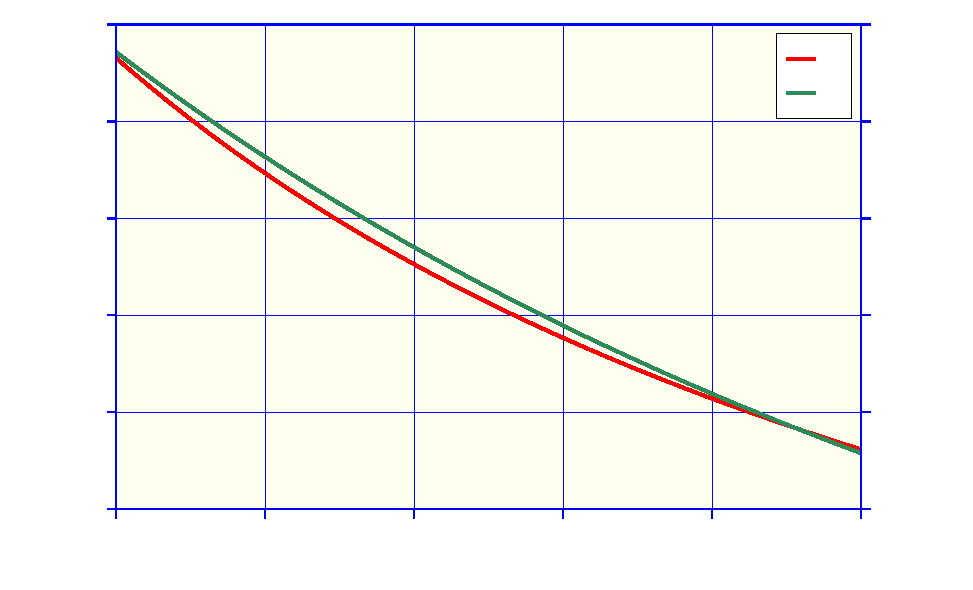
\includegraphics{Cap-Motors-Induccio-Ex8-2-1}}%
    \gplfronttext
  \end{picture}%
\endgroup

	\end{center}
	
	I en la segona s'hi pot veure l'evolució del factor de potència $\cos\varphi$ i del rendiment $\eta$ respecte de la relació entre la tensió aplicada i la tensió nominal $U_1/U\ped{n}$:
	\begin{center}
		% GNUPLOT: LaTeX picture with Postscript
\begingroup
  \makeatletter
  \providecommand\color[2][]{%
    \GenericError{(gnuplot) \space\space\space\@spaces}{%
      Package color not loaded in conjunction with
      terminal option `colourtext'%
    }{See the gnuplot documentation for explanation.%
    }{Either use 'blacktext' in gnuplot or load the package
      color.sty in LaTeX.}%
    \renewcommand\color[2][]{}%
  }%
  \providecommand\includegraphics[2][]{%
    \GenericError{(gnuplot) \space\space\space\@spaces}{%
      Package graphicx or graphics not loaded%
    }{See the gnuplot documentation for explanation.%
    }{The gnuplot epslatex terminal needs graphicx.sty or graphics.sty.}%
    \renewcommand\includegraphics[2][]{}%
  }%
  \providecommand\rotatebox[2]{#2}%
  \@ifundefined{ifGPcolor}{%
    \newif\ifGPcolor
    \GPcolortrue
  }{}%
  \@ifundefined{ifGPblacktext}{%
    \newif\ifGPblacktext
    \GPblacktexttrue
  }{}%
  % define a \g@addto@macro without @ in the name:
  \let\gplgaddtomacro\g@addto@macro
  % define empty templates for all commands taking text:
  \gdef\gplbacktext{}%
  \gdef\gplfronttext{}%
  \makeatother
  \ifGPblacktext
    % no textcolor at all
    \def\colorrgb#1{}%
    \def\colorgray#1{}%
  \else
    % gray or color?
    \ifGPcolor
      \def\colorrgb#1{\color[rgb]{#1}}%
      \def\colorgray#1{\color[gray]{#1}}%
      \expandafter\def\csname LTw\endcsname{\color{white}}%
      \expandafter\def\csname LTb\endcsname{\color{black}}%
      \expandafter\def\csname LTa\endcsname{\color{black}}%
      \expandafter\def\csname LT0\endcsname{\color[rgb]{1,0,0}}%
      \expandafter\def\csname LT1\endcsname{\color[rgb]{0,1,0}}%
      \expandafter\def\csname LT2\endcsname{\color[rgb]{0,0,1}}%
      \expandafter\def\csname LT3\endcsname{\color[rgb]{1,0,1}}%
      \expandafter\def\csname LT4\endcsname{\color[rgb]{0,1,1}}%
      \expandafter\def\csname LT5\endcsname{\color[rgb]{1,1,0}}%
      \expandafter\def\csname LT6\endcsname{\color[rgb]{0,0,0}}%
      \expandafter\def\csname LT7\endcsname{\color[rgb]{1,0.3,0}}%
      \expandafter\def\csname LT8\endcsname{\color[rgb]{0.5,0.5,0.5}}%
    \else
      % gray
      \def\colorrgb#1{\color{black}}%
      \def\colorgray#1{\color[gray]{#1}}%
      \expandafter\def\csname LTw\endcsname{\color{white}}%
      \expandafter\def\csname LTb\endcsname{\color{black}}%
      \expandafter\def\csname LTa\endcsname{\color{black}}%
      \expandafter\def\csname LT0\endcsname{\color{black}}%
      \expandafter\def\csname LT1\endcsname{\color{black}}%
      \expandafter\def\csname LT2\endcsname{\color{black}}%
      \expandafter\def\csname LT3\endcsname{\color{black}}%
      \expandafter\def\csname LT4\endcsname{\color{black}}%
      \expandafter\def\csname LT5\endcsname{\color{black}}%
      \expandafter\def\csname LT6\endcsname{\color{black}}%
      \expandafter\def\csname LT7\endcsname{\color{black}}%
      \expandafter\def\csname LT8\endcsname{\color{black}}%
    \fi
  \fi
    \setlength{\unitlength}{0.0500bp}%
    \ifx\gptboxheight\undefined%
      \newlength{\gptboxheight}%
      \newlength{\gptboxwidth}%
      \newsavebox{\gptboxtext}%
    \fi%
    \setlength{\fboxrule}{0.5pt}%
    \setlength{\fboxsep}{1pt}%
\begin{picture}(9340.00,5660.00)%
    \gplgaddtomacro\gplbacktext{%
      \colorrgb{0.00,0.00,0.00}%%
      \put(849,787){\makebox(0,0)[r]{\strut{} 0,82}}%
      \colorrgb{0.00,0.00,0.00}%%
      \put(849,1950){\makebox(0,0)[r]{\strut{} 0,84}}%
      \colorrgb{0.00,0.00,0.00}%%
      \put(849,3114){\makebox(0,0)[r]{\strut{} 0,86}}%
      \colorrgb{0.00,0.00,0.00}%%
      \put(849,4277){\makebox(0,0)[r]{\strut{} 0,88}}%
      \colorrgb{0.00,0.00,0.00}%%
      \put(849,5440){\makebox(0,0)[r]{\strut{} 0,90}}%
      \colorrgb{0.00,0.00,0.00}%%
      \put(1033,481){\makebox(0,0){\strut{} 0,75}}%
      \colorrgb{0.00,0.00,0.00}%%
      \put(2614,481){\makebox(0,0){\strut{} 0,80}}%
      \colorrgb{0.00,0.00,0.00}%%
      \put(4195,481){\makebox(0,0){\strut{} 0,85}}%
      \colorrgb{0.00,0.00,0.00}%%
      \put(5777,481){\makebox(0,0){\strut{} 0,90}}%
      \colorrgb{0.00,0.00,0.00}%%
      \put(7358,481){\makebox(0,0){\strut{} 0,95}}%
      \colorrgb{0.00,0.00,0.00}%%
      \put(8939,481){\makebox(0,0){\strut{} 1,00}}%
    }%
    \gplgaddtomacro\gplfronttext{%
      \csname LTb\endcsname%%
      \put(255,3113){\rotatebox{-270}{\makebox(0,0){\strut{}$\cos\varphi, \quad \eta$}}}%
      \csname LTb\endcsname%%
      \put(8993,3113){\rotatebox{-270}{\makebox(0,0){\strut{}}}}%
      \csname LTb\endcsname%%
      \put(4986,153){\makebox(0,0){\strut{}$U_1/U\ped{n}$}}%
      \csname LTb\endcsname%%
      \put(4986,5331){\makebox(0,0){\strut{}}}%
      \csname LTb\endcsname%%
      \put(4986,5440){\makebox(0,0){\strut{}}}%
      \csname LTb\endcsname%%
      \put(8289,1530){\makebox(0,0){\strut{}}}%
      \csname LTb\endcsname%%
      \put(8212,1448){\makebox(0,0)[l]{\strut{}$\cos\varphi$}}%
      \csname LTb\endcsname%%
      \put(8212,1120){\makebox(0,0)[l]{\strut{}$\eta$}}%
    }%
    \gplbacktext
    \put(0,0){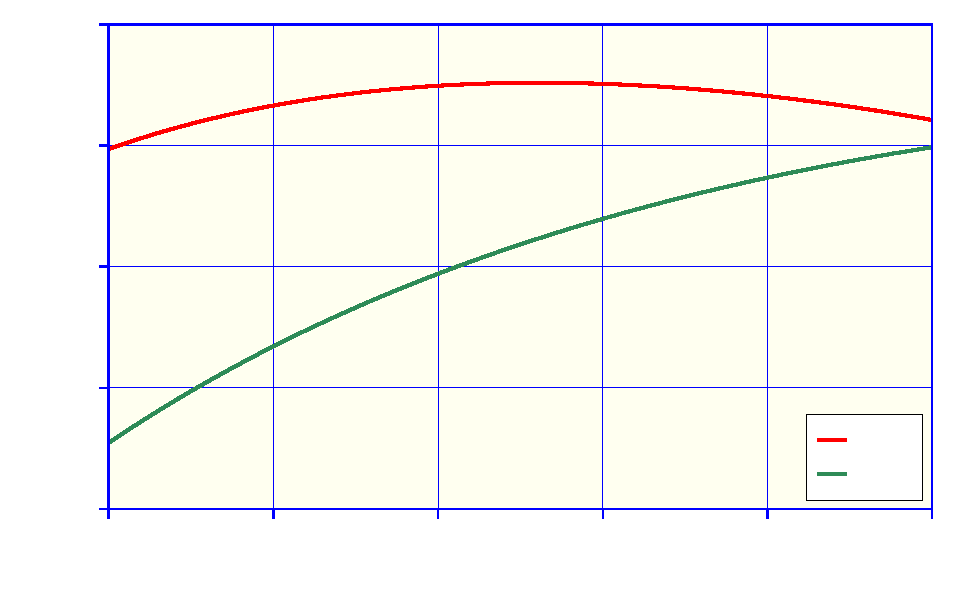
\includegraphics{Cap-Motors-Induccio-Ex8-2-2}}%
    \gplfronttext
  \end{picture}%
\endgroup

	\end{center}
\end{exemple} 


\subsubsection{Arrencada a tensió reduïda, deguda al  corrent d'arrencada mateix}\index{motors d'inducció!arrencada a tensió reduïda, deguda al corrent d'arrencada mateix}

En els apartats anteriors, la tensió d'alimentació al motor $U_1$ sempre s'ha mantingut constant, sigui al seu valor nominal o a un valor reduït. Això vol dir que el sistema d'alimentació que proporciona aquesta tensió és de «potència infinita», és a dir, que pot subministrar qualsevol intensitat de corrent sense que la tensió es vegi afectada.

En la pràctica els sistemes d'alimentació tenen una potència finita i si les càrregues demanen una intensitat de corrent massa elevada, la tensió pot disminuir. En el cas que la càrrega sigui un motor, el corrent d'arrencada, que sol ser elevat, pot ocasionar aquesta disminució de tensió. Un altre element que pot ocasionar una disminució de la tensió és la impedància del cable que connecta el sistema d'alimentació amb el motor.

Un sistema d'alimentació es pot modelar com una font de tensió fase--neutre $U\ped{1,sist}$ en sèrie amb una impedància $Z\ped{sist}$, a partir de la seva tensió fase--fase $U\ped{sist}$ i la seva potència de curtcircuit $S\ped{cc,sist}$:
\begin{align}
	U\ped{1,sist} &= \frac{U\ped{sist}}{\sqrt{3}} \\[1ex]
	Z\ped{sist} &= \frac{U\ped{sist}^2}{S\ped{cc,sist}}
\end{align}

Generalment es pren $\cmplx{U}\ped{1,sist}$ com a fasor de referència, assignant-li un argument igual a zero. 
\begin{equation}
	\cmplx{U}\ped{1,sist} = U\ped{1,sist}
\end{equation}

Pel que fa al fasor  $\cmplx{Z}\ped{sist}$, el valor del seu argument depèn de si es coneix o no el valor de la relació $X/R$ de la potència de curtcircuit, ja que quan aquest valor no és conegut se suposa que la impedància és purament inductiva:
\begin{equation}
	\cmplx{Z}\ped{sist} = 
	\begin{cases}
		\ju Z\ped{sist},  & \quad\text{si no es coneix }\frac{X}{R}  \\[2ex]
		Z\ped{sist} (\cos\varphi+\ju\sin\varphi), \text{ amb } \varphi=\arctan\frac{X}{R}, & \quad\text{si es coneix } \frac{X}{R} 
	\end{cases}
\end{equation}

Per tant, a partir dels valors $\cmplx{U}\ped{1,sist}$ i $\cmplx{Z}\ped{sist}$, de la impedància per fase del cable $\cmplx{Z}\ped{cable}$, i de la impedància del motor $\cmplx{Z}\ped{mot}(s)$ segons l'equació \eqref{eq:mot-Zmot}, podem representar el circuit equivalent de la Figura \vref{pic:mot-esq-equiv-U-Sist}:
\begin{center}
	\input{Imatges/Cap-Motors-Induccio-Esq-Equiv-U-Sist.pdf_tex}
	\captionof{figure}{Esquema equivalent d'un motor alimentat per un sistema de potència}
	\label{pic:mot-esq-equiv-U-Sist}
\end{center}

A partir d'aquest circuit, podem obtenir  el valor de la tensió d'alimentació del motor, la qual deixa de ser fixa i passa a dependre del  lliscament:
\begin{equation}
	\cmplx{U}_1(s) = \frac{\cmplx{Z}\ped{mot}(s)}{\cmplx{Z}\ped{sist} + \cmplx{Z}\ped{cable} +  \cmplx{Z}\ped{mot}(s)} \cmplx{U}\ped{1,sist}\label{eq:mot-U-redu}
\end{equation}

El mòdul d'aquesta tensió és:
\begin{equation}
	U_1(s) = \frac{Z\ped{mot}(s)}{|\cmplx{Z}\ped{sist} + \cmplx{Z}\ped{cable} +  \cmplx{Z}\ped{mot}(s)|} U\ped{1,sist}
\end{equation}

Totes les equacions que s'han desenvolupat en les seccions anteriors segueixen sent vàlides, simplement substituint $\cmplx{U}_1$ o $U_1$ per  $\cmplx{U}_1(s)$ o $U_1(s)$ respectivament. Per exemple, les equacions del corrent de l'estator $\cmplx{I}_1(s)$ i del parell mecànic $T\ped{m}(s)$ esdevenen:
\begin{subequations}
	\begin{align}
	\cmplx{I}_1(s) &= \frac{\cmplx{U}_1(s)}{\cmplx{Z}\ped{mot}(s)} = \frac{\cmplx{U}\ped{1,sist}}{\cmplx{Z}\ped{sist} + \cmplx{Z}\ped{cable} +  \cmplx{Z}\ped{mot}(s)} \label{eq:mot-I-redu} \\[1ex]
	T\ped{m}(s)  &= \frac{3 R_2}{s\,\omega\ped{m,sinc}} Y\ped{eq}^2(s) U_1^2(s) =
	\frac{3 R_2}{s\,\omega\ped{m,sinc}} Y\ped{eq}^2(s) \left(\frac{Z\ped{mot}(s)}{|\cmplx{Z}\ped{sist} + \cmplx{Z}\ped{cable} +  \cmplx{Z}\ped{mot}(s)|} \right)^2 U\ped{1,sist}^2 \label{eq:mot-Tm-redu}
	\end{align}
\end{subequations}

Les úniques equacions que canvien són les \eqref{eq:mot-ZTh} i  \eqref{eq:mot-UTh}, les quals defineixen el circuit  equivalent Thévenin que veu el rotor. Aquestes equacions es converteixen en les següents:\index{ETh@$\cmplx{E}\ped{Th}$}\index{ZTh@$\cmplx{Z}\ped{Th}$}
\begin{subequations}
	\begin{align}
	\cmplx{Z}\ped{Th} &= \frac{(\cmplx{Z}\ped{sist} + \cmplx{Z}\ped{cable} + R_1 + \ju X_1) \cmplx{Z}_0}{\cmplx{Z}\ped{sist} + \cmplx{Z}\ped{cable} + R_1 + \ju X_1 + \cmplx{Z}_0} \label{eq:mot-ZTh-redu}\\[1ex]
	\cmplx{E}\ped{Th} &= \frac{\cmplx{Z}_0}{\cmplx{Z}\ped{sist} + \cmplx{Z}\ped{cable} + R_1 + \ju X_1 + \cmplx{Z}_0} \cmplx{U}\ped{1,sist} \label{eq:mot-UTh-redu}
	\end{align}
\end{subequations}

\begin{exemple}[Arrencada a tensió reduïda, deguda al  corrent d'arrencada mateix]
	\addcontentsxms{Arrencada a tensió reduïda, deguda al  corrent d'arrencada mateix}
	Partim del mateix motor de l'exemple \vref{ex:mot} i del mateix ventilador utilitzat en l'exemple \vref{ex:mot-tens-redu}. El motor està connectat a un sistema d'alimentació trifàsic de característiques: $U\ped{sist}=\qty{380}{V}$, $S\ped{cc,sist}=\qty{5}{MVA}$, $X/R=9$ i $f=\qty{50}{Hz}$. El cable que connecta aquest sistema amb el motor és de \qty{6}{mm^2}, té una longitud de:  $L=\qty{80}{m}$, i una impedància de: $\cmplx{Z} = \complexqty{3,960+j0,123}{\ohm/km}$. Es tracta de trobar les característiques de funcionament del motor.
	
	La tensió fase--neutre del sistema es pren com a fasor de referència, i val:
	\[
		\cmplx{U}\ped{1,sist} = \frac{\qty{380}{V}}{\sqrt{3}} = \qtypd{219,393}{0}{V}
	\]
	
	La impedància equivalent del sistema val:
	\[
		\cmplx{Z}\ped{sist} = \frac{(\qty{380}{V})^2}{\qty{5e6}{VA}} \times (\cos(\arctan 9) + \ju \sin(\arctan 9)) = \complexqty{0,003+j0,029}{\ohm}	
	\]
	
	La impedància total del cable val:
	\[
		\cmplx{Z}\ped{cable} = \qty{80e-3}{km} \times \complexqty{3,960+j0,123}{\ohm/km} = \complexqty{0,317+j0,010}{\ohm}
	\]
	
	Els valors de $\omega\ped{m,sinc}$ i $\cmplx{Z}_0$, els quals no depenen del lliscament, s'han calculat en  l'exemple \ref{ex:mot} i valen:
	\begin{align*}
		\omega\ped{m,sinc} &=  \qty{157,080}{rad/s} \\
		\cmplx{Z}_0 &=  \complexqty{4,390+j39,512}{\ohm} 
	\end{align*}
		
	L'equació de $\cmplx{Z}\ped{mot}(s)$ també és la mateixa que s'ha calculat en l'exemple  \ref{ex:mot}, ja que només depèn dels paràmetres del motor:
	\[
		\cmplx{Z}\ped{mot}(s) = \complexqty{0,5+j1,5}{\ohm} + \frac{\complexqty{4,390+j39,512}{\ohm}\,\times\,
		\left(\tfrac{\qty{0,625}{\ohm}}{s}\, + \, \complexqty{j1,25}{\ohm}\right)}{\complexqty{4,390+j39,512}{\ohm}\,+\,
		\tfrac{\qty{0,625}{\ohm}}{s}\, + \,\complexqty{j1,25}{\ohm}}  
	\] 
	
	En canvi, la tensió aplicada al motor $\cmplx{U}_1$ passa a dependre del lliscament segons l'equació \eqref{eq:mot-U-redu}:
	\[
		\cmplx{U}_1(s) = \frac{\cmplx{Z}\ped{mot}(s)}{\complexqty{0,003+j0,029}{\ohm} + \complexqty{0,317+j0,010}{\ohm}  +  \cmplx{Z}\ped{mot}(s)} \times \qtypd{219,393}{0}{V}
	\]
	
	Igualment, per calcular  la impedància $\cmplx{Z}\ped{Th}$ i la tensió $\cmplx{E}\ped{Th}$ Thévenin equivalents hem d'utilitzar les equacions \eqref{eq:mot-ZTh-redu} i \eqref{eq:mot-UTh-redu}:
	\begin{align*}
		\cmplx{Z}\ped{Th} &= \frac{(\complexqty{0,003+j0,029}{\ohm} + \complexqty{0,317+j0,010}{\ohm} +  \complexqty{0,5+j1,5}{\ohm})\times\complexqty{4,390+j39,512}{\ohm}}
		{\complexqty{0,003+j0,029}{\ohm} + \complexqty{0,317+j0,010}{\ohm} + \complexqty{0,5+j1,5}{\ohm}+\complexqty{4,390+j39,512}{\ohm}}  \\[1ex]   
		&= \complexqty{0,765+j1,490}{\ohm}
	\end{align*}
	\vspace{-5mm}
	\begin{align*}		
		\cmplx{E}\ped{Th}  &= \frac{\complexqty{4,390+j39,512}{\ohm}}
		{\complexqty{0,003+j0,029}{\ohm} + \complexqty{0,317+j0,010}{\ohm} + \complexqty{0,5+j1,5}{\ohm}+\complexqty{4,390+j39,512}{\ohm}}\times\qtypd{219,393}{0}{V}  \\[1ex]   
		&=  \qtypd{210,779}{0,8932}{V}
	\end{align*}
	
	L'equació de la corba parell-velocitat en newton metre del ventilador, és la mateixa que s'ha calculat en l'exemple  \ref{ex:mot-tens-redu}:
	\[
		T\ped{load}(s) = 3{,}2 (1-s) + 58{,}9 (1-s)^2
	\]
	
	Podem ara substituir els  valors calculats fins ara en l'equació \eqref{eq:Tload-U1-Yeq} i resoldre-la; cal recordar que en lloc de $U_1$ hem de posar-hi l'equació de $U_1(s)$ que acabem de calcular. Aquesta equació és clarament no lineal, i per tal de resoldre-la cal utilitzar programes de càlcul o mètodes numèrics, com ara els explicats en l'apèndix \ref{sec:func-no-lin}. La solució és:
	\[
		s = 0{,}048
	\]
	
	Aquest lliscament correspon a la velocitat següent:
	\[
		n= (1-\num{0,048})\times \qty{1500}{r/min} = \qty{1428}{r/min}
	\]
	
	Utilitzant les equacions \eqref{eq:mot-I-redu} i \eqref{eq:mot-Tm-redu} amb $s=0{,}048$ i $s=1$, trobem els valors del corrent i del parell mecànic, en el punt de funcionament nominal i en l'arrencada respectivament:
	\begin{align*}
		I\ped{1,n} &= \qty{16,9}{A} &
		I\ped{1,arr} &= \qty{70,9}{A} \\[1ex] 
		T\ped{m,n} &=  \qty{56,4}{N.m} &	
		T\ped{m,arr} &=  \qty{56,2}{N.m}
	\end{align*}
	
	Utilitzant l'equació \eqref{eq:mot-U-redu} amb $s=0{,}048$ trobem el valor de la tensió en el motor, en el punt de funcionament nominal:
	\[
		\cmplx{U}\ped{1,n} = \qtypd{214,305}{0,5019}{V}
	\]
	
	Calculem ara el lliscament en el punt de parell màxim, segons l'equació \eqref{eq:s-T-max}:
	\[
		s_{T\ped{m,\text{màx}}} =  \frac{\qty{0,625}{\ohm}}{|\complexqty{0,765+j1,490}{\ohm} + \complexqty{j1,25}{\ohm}|} = \num{0,2197} 
	\]
	
	Aquest lliscament correspon a la següent  velocitat del motor:
	\[
		n_{\text{m},T\ped{m,\text{màx}}} = (1 - 0{,}2197) \times \qty{1500}{r/min} = \qty{1170,5}{r/min}
	\]
	
	Utilitzant l'equació  \eqref{eq:mot-Tm-redu} amb $s=0{,}2197$, trobarem el valor del parell mecànic màxim  $T\ped{m,\text{màx}}$:
	\[
		T\ped{m,\text{màx}} = \qty{117,5}{N.m}
	\]
	Representem ara la gràfica de l'evolució dels parells $T\ped{load}$ i   $T\ped{m}$, i del	corrent $I_1$ respecte de la velocitat $n\ped{m}$, indicant-hi els valors en el punt nominal de funcionament i en el punt de parell màxim:
	
	\begin{center}
		\fontsize{10pt}{11pt}\selectfont
		% GNUPLOT: LaTeX picture with Postscript
\begingroup
  \makeatletter
  \providecommand\color[2][]{%
    \GenericError{(gnuplot) \space\space\space\@spaces}{%
      Package color not loaded in conjunction with
      terminal option `colourtext'%
    }{See the gnuplot documentation for explanation.%
    }{Either use 'blacktext' in gnuplot or load the package
      color.sty in LaTeX.}%
    \renewcommand\color[2][]{}%
  }%
  \providecommand\includegraphics[2][]{%
    \GenericError{(gnuplot) \space\space\space\@spaces}{%
      Package graphicx or graphics not loaded%
    }{See the gnuplot documentation for explanation.%
    }{The gnuplot epslatex terminal needs graphicx.sty or graphics.sty.}%
    \renewcommand\includegraphics[2][]{}%
  }%
  \providecommand\rotatebox[2]{#2}%
  \@ifundefined{ifGPcolor}{%
    \newif\ifGPcolor
    \GPcolortrue
  }{}%
  \@ifundefined{ifGPblacktext}{%
    \newif\ifGPblacktext
    \GPblacktexttrue
  }{}%
  % define a \g@addto@macro without @ in the name:
  \let\gplgaddtomacro\g@addto@macro
  % define empty templates for all commands taking text:
  \gdef\gplbacktext{}%
  \gdef\gplfronttext{}%
  \makeatother
  \ifGPblacktext
    % no textcolor at all
    \def\colorrgb#1{}%
    \def\colorgray#1{}%
  \else
    % gray or color?
    \ifGPcolor
      \def\colorrgb#1{\color[rgb]{#1}}%
      \def\colorgray#1{\color[gray]{#1}}%
      \expandafter\def\csname LTw\endcsname{\color{white}}%
      \expandafter\def\csname LTb\endcsname{\color{black}}%
      \expandafter\def\csname LTa\endcsname{\color{black}}%
      \expandafter\def\csname LT0\endcsname{\color[rgb]{1,0,0}}%
      \expandafter\def\csname LT1\endcsname{\color[rgb]{0,1,0}}%
      \expandafter\def\csname LT2\endcsname{\color[rgb]{0,0,1}}%
      \expandafter\def\csname LT3\endcsname{\color[rgb]{1,0,1}}%
      \expandafter\def\csname LT4\endcsname{\color[rgb]{0,1,1}}%
      \expandafter\def\csname LT5\endcsname{\color[rgb]{1,1,0}}%
      \expandafter\def\csname LT6\endcsname{\color[rgb]{0,0,0}}%
      \expandafter\def\csname LT7\endcsname{\color[rgb]{1,0.3,0}}%
      \expandafter\def\csname LT8\endcsname{\color[rgb]{0.5,0.5,0.5}}%
    \else
      % gray
      \def\colorrgb#1{\color{black}}%
      \def\colorgray#1{\color[gray]{#1}}%
      \expandafter\def\csname LTw\endcsname{\color{white}}%
      \expandafter\def\csname LTb\endcsname{\color{black}}%
      \expandafter\def\csname LTa\endcsname{\color{black}}%
      \expandafter\def\csname LT0\endcsname{\color{black}}%
      \expandafter\def\csname LT1\endcsname{\color{black}}%
      \expandafter\def\csname LT2\endcsname{\color{black}}%
      \expandafter\def\csname LT3\endcsname{\color{black}}%
      \expandafter\def\csname LT4\endcsname{\color{black}}%
      \expandafter\def\csname LT5\endcsname{\color{black}}%
      \expandafter\def\csname LT6\endcsname{\color{black}}%
      \expandafter\def\csname LT7\endcsname{\color{black}}%
      \expandafter\def\csname LT8\endcsname{\color{black}}%
    \fi
  \fi
    \setlength{\unitlength}{0.0500bp}%
    \ifx\gptboxheight\undefined%
      \newlength{\gptboxheight}%
      \newlength{\gptboxwidth}%
      \newsavebox{\gptboxtext}%
    \fi%
    \setlength{\fboxrule}{0.5pt}%
    \setlength{\fboxsep}{1pt}%
\begin{picture}(9340.00,5660.00)%
    \gplgaddtomacro\gplbacktext{%
      \colorrgb{0.00,0.00,0.00}%%
      \put(752,787){\makebox(0,0)[r]{\strut{} 0}}%
      \colorrgb{0.00,0.00,0.00}%%
      \put(752,1097){\makebox(0,0)[r]{\strut{} 10}}%
      \colorrgb{0.00,0.00,0.00}%%
      \put(752,1407){\makebox(0,0)[r]{\strut{} 20}}%
      \colorrgb{0.00,0.00,0.00}%%
      \put(752,1718){\makebox(0,0)[r]{\strut{} 30}}%
      \colorrgb{0.00,0.00,0.00}%%
      \put(752,2028){\makebox(0,0)[r]{\strut{} 40}}%
      \colorrgb{0.00,0.00,0.00}%%
      \put(752,2338){\makebox(0,0)[r]{\strut{} 50}}%
      \colorrgb{0.00,0.00,0.00}%%
      \put(752,2648){\makebox(0,0)[r]{\strut{} 60}}%
      \colorrgb{0.00,0.00,0.00}%%
      \put(752,2958){\makebox(0,0)[r]{\strut{} 70}}%
      \colorrgb{0.00,0.00,0.00}%%
      \put(752,3269){\makebox(0,0)[r]{\strut{} 80}}%
      \colorrgb{0.00,0.00,0.00}%%
      \put(752,3579){\makebox(0,0)[r]{\strut{} 90}}%
      \colorrgb{0.00,0.00,0.00}%%
      \put(752,3889){\makebox(0,0)[r]{\strut{} 100}}%
      \colorrgb{0.00,0.00,0.00}%%
      \put(752,4199){\makebox(0,0)[r]{\strut{} 110}}%
      \colorrgb{0.00,0.00,0.00}%%
      \put(752,4509){\makebox(0,0)[r]{\strut{} 120}}%
      \colorrgb{0.00,0.00,0.00}%%
      \put(752,4820){\makebox(0,0)[r]{\strut{} 130}}%
      \colorrgb{0.00,0.00,0.00}%%
      \put(752,5130){\makebox(0,0)[r]{\strut{} 140}}%
      \colorrgb{0.00,0.00,0.00}%%
      \put(752,5440){\makebox(0,0)[r]{\strut{} 150}}%
      \colorrgb{0.00,0.00,0.00}%%
      \put(936,481){\makebox(0,0){\strut{} 0}}%
      \colorrgb{0.00,0.00,0.00}%%
      \put(1424,481){\makebox(0,0){\strut{} 100}}%
      \colorrgb{0.00,0.00,0.00}%%
      \put(1912,481){\makebox(0,0){\strut{} 200}}%
      \colorrgb{0.00,0.00,0.00}%%
      \put(2400,481){\makebox(0,0){\strut{} 300}}%
      \colorrgb{0.00,0.00,0.00}%%
      \put(2888,481){\makebox(0,0){\strut{} 400}}%
      \colorrgb{0.00,0.00,0.00}%%
      \put(3376,481){\makebox(0,0){\strut{} 500}}%
      \colorrgb{0.00,0.00,0.00}%%
      \put(3864,481){\makebox(0,0){\strut{} 600}}%
      \colorrgb{0.00,0.00,0.00}%%
      \put(4352,481){\makebox(0,0){\strut{} 700}}%
      \colorrgb{0.00,0.00,0.00}%%
      \put(4841,481){\makebox(0,0){\strut{} 800}}%
      \colorrgb{0.00,0.00,0.00}%%
      \put(5329,481){\makebox(0,0){\strut{} 900}}%
      \colorrgb{0.00,0.00,0.00}%%
      \put(5817,481){\makebox(0,0){\strut{} 1000}}%
      \colorrgb{0.00,0.00,0.00}%%
      \put(6305,481){\makebox(0,0){\strut{} 1100}}%
      \colorrgb{0.00,0.00,0.00}%%
      \put(6793,481){\makebox(0,0){\strut{} 1200}}%
      \colorrgb{0.00,0.00,0.00}%%
      \put(7281,481){\makebox(0,0){\strut{} 1300}}%
      \colorrgb{0.00,0.00,0.00}%%
      \put(7769,481){\makebox(0,0){\strut{} 1400}}%
      \colorrgb{0.00,0.00,0.00}%%
      \put(8257,481){\makebox(0,0){\strut{} 1500}}%
      \colorrgb{0.00,0.00,0.00}%%
      \put(8441,787){\makebox(0,0)[l]{\strut{} 0}}%
      \colorrgb{0.00,0.00,0.00}%%
      \put(8441,1097){\makebox(0,0)[l]{\strut{} 5}}%
      \colorrgb{0.00,0.00,0.00}%%
      \put(8441,1407){\makebox(0,0)[l]{\strut{} 10}}%
      \colorrgb{0.00,0.00,0.00}%%
      \put(8441,1718){\makebox(0,0)[l]{\strut{} 15}}%
      \colorrgb{0.00,0.00,0.00}%%
      \put(8441,2028){\makebox(0,0)[l]{\strut{} 20}}%
      \colorrgb{0.00,0.00,0.00}%%
      \put(8441,2338){\makebox(0,0)[l]{\strut{} 25}}%
      \colorrgb{0.00,0.00,0.00}%%
      \put(8441,2648){\makebox(0,0)[l]{\strut{} 30}}%
      \colorrgb{0.00,0.00,0.00}%%
      \put(8441,2958){\makebox(0,0)[l]{\strut{} 35}}%
      \colorrgb{0.00,0.00,0.00}%%
      \put(8441,3269){\makebox(0,0)[l]{\strut{} 40}}%
      \colorrgb{0.00,0.00,0.00}%%
      \put(8441,3579){\makebox(0,0)[l]{\strut{} 45}}%
      \colorrgb{0.00,0.00,0.00}%%
      \put(8441,3889){\makebox(0,0)[l]{\strut{} 50}}%
      \colorrgb{0.00,0.00,0.00}%%
      \put(8441,4199){\makebox(0,0)[l]{\strut{} 55}}%
      \colorrgb{0.00,0.00,0.00}%%
      \put(8441,4509){\makebox(0,0)[l]{\strut{} 60}}%
      \colorrgb{0.00,0.00,0.00}%%
      \put(8441,4820){\makebox(0,0)[l]{\strut{} 65}}%
      \colorrgb{0.00,0.00,0.00}%%
      \put(8441,5130){\makebox(0,0)[l]{\strut{} 70}}%
      \colorrgb{0.00,0.00,0.00}%%
      \put(8441,5440){\makebox(0,0)[l]{\strut{} 75}}%
    }%
    \gplgaddtomacro\gplfronttext{%
      \csname LTb\endcsname%%
      \put(255,3113){\rotatebox{-270}{\makebox(0,0){\strut{}$T\ped{m}\, / \,\si{N.m}, \quad T\ped{load}\, / \,\si{N.m}$}}}%
      \csname LTb\endcsname%%
      \put(8938,3113){\rotatebox{-270}{\makebox(0,0){\strut{}$I_1\, / \,\si{A}$}}}%
      \csname LTb\endcsname%%
      \put(4596,153){\makebox(0,0){\strut{}$n\ped{m}\, / \,\si{r/min}$}}%
      \csname LTb\endcsname%%
      \put(4596,5331){\makebox(0,0){\strut{}}}%
      \csname LTb\endcsname%%
      \put(4596,5440){\makebox(0,0){\strut{}}}%
      \csname LTb\endcsname%%
      \put(7728,5189){\makebox(0,0){\strut{}}}%
      \csname LTb\endcsname%%
      \put(7675,5107){\makebox(0,0)[l]{\strut{}$T\ped{load}$}}%
      \csname LTb\endcsname%%
      \put(7675,4779){\makebox(0,0)[l]{\strut{}$T\ped{m}$}}%
      \csname LTb\endcsname%%
      \put(7675,4451){\makebox(0,0)[l]{\strut{}$I_1$}}%
      \csname LTb\endcsname%%
      \put(1668,2416){\makebox(0,0){$\scriptstyle\SI{56,4}{N.m}$}}%
      \csname LTb\endcsname%%
      \put(7828,1345){\rotatebox{-270}{\makebox(0,0){$\scriptstyle\SI{1428}{r/min}$}}}%
      \csname LTb\endcsname%%
      \put(1668,4298){\makebox(0,0){$\scriptstyle\SI{117,5}{N.m}$}}%
      \csname LTb\endcsname%%
      \put(6573,1407){\rotatebox{-270}{\makebox(0,0){$\scriptstyle\SI{1170,5}{r/min}$}}}%
      \csname LTb\endcsname%%
      \put(7427,1904){\makebox(0,0){$\scriptstyle\SI{16,9}{A}$}}%
    }%
    \gplbacktext
    \put(0,0){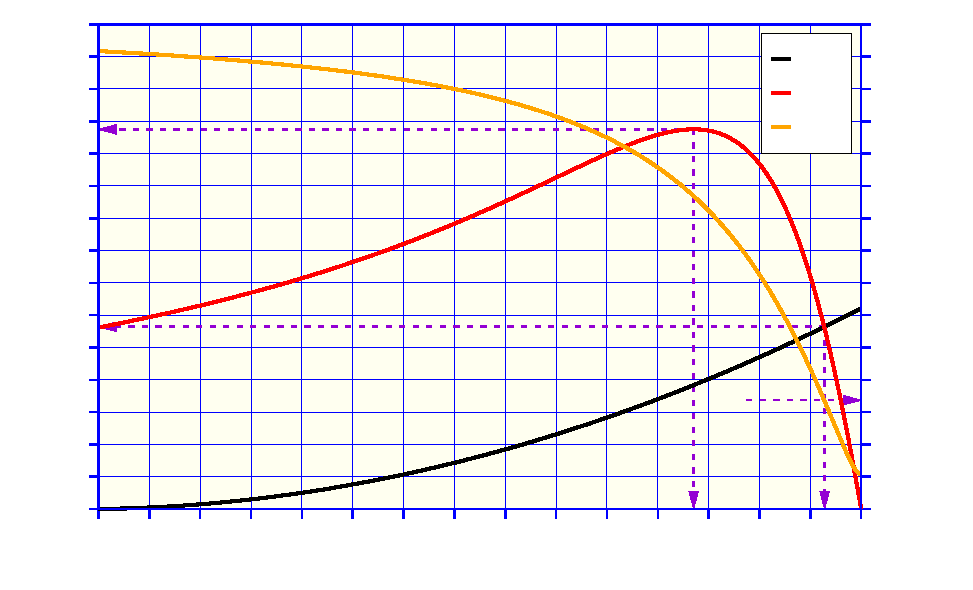
\includegraphics{Cap-Motors-Induccio-Ex9-1}}%
    \gplfronttext
  \end{picture}%
\endgroup

	\end{center}

	Representem per acabar, la tensió $U\ped{1,sist}$ i la gràfica de l'evolució de la tensió $U_1$ respecte de la velocitat $n\ped{m}$, indicant-hi els valors en el punt nominal de funcionament:
	
	\begin{center}
		\fontsize{10pt}{11pt}\selectfont
		% GNUPLOT: LaTeX picture with Postscript
\begingroup
  \makeatletter
  \providecommand\color[2][]{%
    \GenericError{(gnuplot) \space\space\space\@spaces}{%
      Package color not loaded in conjunction with
      terminal option `colourtext'%
    }{See the gnuplot documentation for explanation.%
    }{Either use 'blacktext' in gnuplot or load the package
      color.sty in LaTeX.}%
    \renewcommand\color[2][]{}%
  }%
  \providecommand\includegraphics[2][]{%
    \GenericError{(gnuplot) \space\space\space\@spaces}{%
      Package graphicx or graphics not loaded%
    }{See the gnuplot documentation for explanation.%
    }{The gnuplot epslatex terminal needs graphicx.sty or graphics.sty.}%
    \renewcommand\includegraphics[2][]{}%
  }%
  \providecommand\rotatebox[2]{#2}%
  \@ifundefined{ifGPcolor}{%
    \newif\ifGPcolor
    \GPcolortrue
  }{}%
  \@ifundefined{ifGPblacktext}{%
    \newif\ifGPblacktext
    \GPblacktexttrue
  }{}%
  % define a \g@addto@macro without @ in the name:
  \let\gplgaddtomacro\g@addto@macro
  % define empty templates for all commands taking text:
  \gdef\gplbacktext{}%
  \gdef\gplfronttext{}%
  \makeatother
  \ifGPblacktext
    % no textcolor at all
    \def\colorrgb#1{}%
    \def\colorgray#1{}%
  \else
    % gray or color?
    \ifGPcolor
      \def\colorrgb#1{\color[rgb]{#1}}%
      \def\colorgray#1{\color[gray]{#1}}%
      \expandafter\def\csname LTw\endcsname{\color{white}}%
      \expandafter\def\csname LTb\endcsname{\color{black}}%
      \expandafter\def\csname LTa\endcsname{\color{black}}%
      \expandafter\def\csname LT0\endcsname{\color[rgb]{1,0,0}}%
      \expandafter\def\csname LT1\endcsname{\color[rgb]{0,1,0}}%
      \expandafter\def\csname LT2\endcsname{\color[rgb]{0,0,1}}%
      \expandafter\def\csname LT3\endcsname{\color[rgb]{1,0,1}}%
      \expandafter\def\csname LT4\endcsname{\color[rgb]{0,1,1}}%
      \expandafter\def\csname LT5\endcsname{\color[rgb]{1,1,0}}%
      \expandafter\def\csname LT6\endcsname{\color[rgb]{0,0,0}}%
      \expandafter\def\csname LT7\endcsname{\color[rgb]{1,0.3,0}}%
      \expandafter\def\csname LT8\endcsname{\color[rgb]{0.5,0.5,0.5}}%
    \else
      % gray
      \def\colorrgb#1{\color{black}}%
      \def\colorgray#1{\color[gray]{#1}}%
      \expandafter\def\csname LTw\endcsname{\color{white}}%
      \expandafter\def\csname LTb\endcsname{\color{black}}%
      \expandafter\def\csname LTa\endcsname{\color{black}}%
      \expandafter\def\csname LT0\endcsname{\color{black}}%
      \expandafter\def\csname LT1\endcsname{\color{black}}%
      \expandafter\def\csname LT2\endcsname{\color{black}}%
      \expandafter\def\csname LT3\endcsname{\color{black}}%
      \expandafter\def\csname LT4\endcsname{\color{black}}%
      \expandafter\def\csname LT5\endcsname{\color{black}}%
      \expandafter\def\csname LT6\endcsname{\color{black}}%
      \expandafter\def\csname LT7\endcsname{\color{black}}%
      \expandafter\def\csname LT8\endcsname{\color{black}}%
    \fi
  \fi
    \setlength{\unitlength}{0.0500bp}%
    \ifx\gptboxheight\undefined%
      \newlength{\gptboxheight}%
      \newlength{\gptboxwidth}%
      \newsavebox{\gptboxtext}%
    \fi%
    \setlength{\fboxrule}{0.5pt}%
    \setlength{\fboxsep}{1pt}%
\begin{picture}(9340.00,5660.00)%
    \gplgaddtomacro\gplbacktext{%
      \colorrgb{0.00,0.00,0.00}%%
      \put(752,787){\makebox(0,0)[r]{\strut{} 204}}%
      \colorrgb{0.00,0.00,0.00}%%
      \put(752,1369){\makebox(0,0)[r]{\strut{} 206}}%
      \colorrgb{0.00,0.00,0.00}%%
      \put(752,1950){\makebox(0,0)[r]{\strut{} 208}}%
      \colorrgb{0.00,0.00,0.00}%%
      \put(752,2532){\makebox(0,0)[r]{\strut{} 210}}%
      \colorrgb{0.00,0.00,0.00}%%
      \put(752,3114){\makebox(0,0)[r]{\strut{} 212}}%
      \colorrgb{0.00,0.00,0.00}%%
      \put(752,3695){\makebox(0,0)[r]{\strut{} 214}}%
      \colorrgb{0.00,0.00,0.00}%%
      \put(752,4277){\makebox(0,0)[r]{\strut{} 216}}%
      \colorrgb{0.00,0.00,0.00}%%
      \put(752,4858){\makebox(0,0)[r]{\strut{} 218}}%
      \colorrgb{0.00,0.00,0.00}%%
      \put(752,5440){\makebox(0,0)[r]{\strut{} 220}}%
      \colorrgb{0.00,0.00,0.00}%%
      \put(936,481){\makebox(0,0){\strut{} 0}}%
      \colorrgb{0.00,0.00,0.00}%%
      \put(1470,481){\makebox(0,0){\strut{} 100}}%
      \colorrgb{0.00,0.00,0.00}%%
      \put(2003,481){\makebox(0,0){\strut{} 200}}%
      \colorrgb{0.00,0.00,0.00}%%
      \put(2537,481){\makebox(0,0){\strut{} 300}}%
      \colorrgb{0.00,0.00,0.00}%%
      \put(3070,481){\makebox(0,0){\strut{} 400}}%
      \colorrgb{0.00,0.00,0.00}%%
      \put(3604,481){\makebox(0,0){\strut{} 500}}%
      \colorrgb{0.00,0.00,0.00}%%
      \put(4137,481){\makebox(0,0){\strut{} 600}}%
      \colorrgb{0.00,0.00,0.00}%%
      \put(4671,481){\makebox(0,0){\strut{} 700}}%
      \colorrgb{0.00,0.00,0.00}%%
      \put(5204,481){\makebox(0,0){\strut{} 800}}%
      \colorrgb{0.00,0.00,0.00}%%
      \put(5738,481){\makebox(0,0){\strut{} 900}}%
      \colorrgb{0.00,0.00,0.00}%%
      \put(6271,481){\makebox(0,0){\strut{} 1000}}%
      \colorrgb{0.00,0.00,0.00}%%
      \put(6805,481){\makebox(0,0){\strut{} 1100}}%
      \colorrgb{0.00,0.00,0.00}%%
      \put(7338,481){\makebox(0,0){\strut{} 1200}}%
      \colorrgb{0.00,0.00,0.00}%%
      \put(7872,481){\makebox(0,0){\strut{} 1300}}%
      \colorrgb{0.00,0.00,0.00}%%
      \put(8405,481){\makebox(0,0){\strut{} 1400}}%
      \colorrgb{0.00,0.00,0.00}%%
      \put(8939,481){\makebox(0,0){\strut{} 1500}}%
    }%
    \gplgaddtomacro\gplfronttext{%
      \csname LTb\endcsname%%
      \put(255,3113){\rotatebox{-270}{\makebox(0,0){\strut{}$U_1\, / \,\si{V}, \quad U\ped{1,sist}\, / \,\si{V}$}}}%
      \csname LTb\endcsname%%
      \put(8993,3113){\rotatebox{-270}{\makebox(0,0){\strut{}}}}%
      \csname LTb\endcsname%%
      \put(4937,153){\makebox(0,0){\strut{}$n\ped{m}\, / \,\si{r/min}$}}%
      \csname LTb\endcsname%%
      \put(4937,5331){\makebox(0,0){\strut{}}}%
      \csname LTb\endcsname%%
      \put(4937,5440){\makebox(0,0){\strut{}}}%
      \csname LTb\endcsname%%
      \put(7622,4840){\makebox(0,0){\strut{}}}%
      \csname LTb\endcsname%%
      \put(7448,4758){\makebox(0,0)[l]{\strut{}$U_1$}}%
      \csname LTb\endcsname%%
      \put(7448,4430){\makebox(0,0)[l]{\strut{}$U\ped{1,sist}$}}%
      \csname LTb\endcsname%%
      \put(1736,3870){\makebox(0,0){$\scriptstyle\SI{214,305}{V}$}}%
      \csname LTb\endcsname%%
      \put(8469,1369){\rotatebox{-270}{\makebox(0,0){$\scriptstyle\SI{1428}{r/min}$}}}%
    }%
    \gplbacktext
    \put(0,0){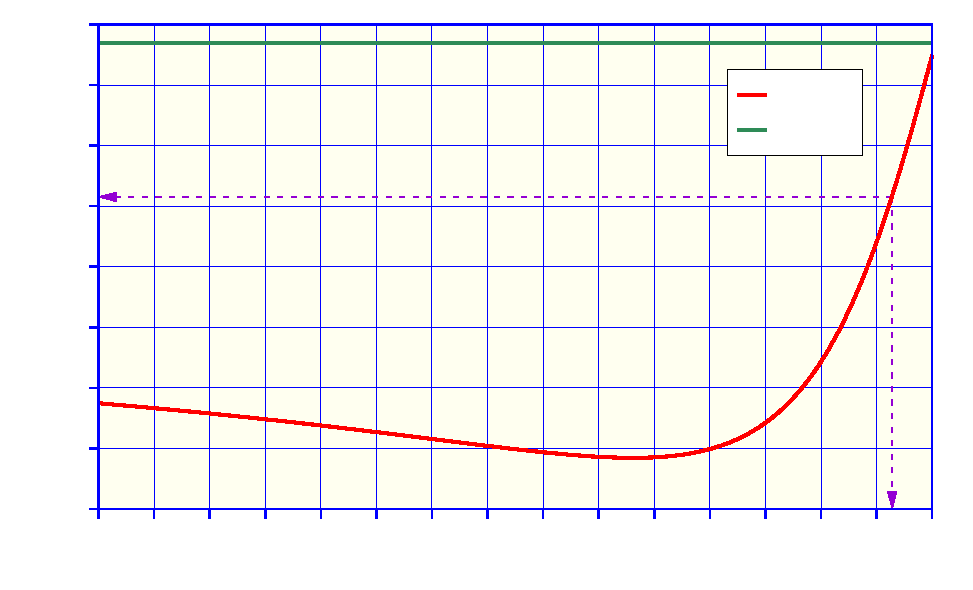
\includegraphics{Cap-Motors-Induccio-Ex9-2}}%
    \gplfronttext
  \end{picture}%
\endgroup

	\end{center}

\end{exemple}	

	    
\section{Norma NEMA MG-1}\index{NEMA!MG-1}

La \textit{National Electrical Manufacturers Associatio}n (NEMA),
tracta en la norma  MG-1 \textit{Motors and Generators} una gran quantitat de qüestions de tota mena relatives a motors i generadors, tant trifàsics com monofàsics, de corrent continu i de corrent altern.

S'expliquen a continuació algunes de les qüestions d'aquesta norma que són d'aplicació als motors d'inducció trifàsics.

\subsection{Punts característics de la corba parell-velocitat}
\index{NEMA!MG-1!punts característics en la corba parell-velocitat}

En la Figura \vref{pic:mot-punts-T-vel} es representa una corba típica parell-velocitat d'un motor, assenyalant-hi quatre punts als quals la norma NEMA MG-1 els dona uns noms característics. En l'eix d'abscisses s'hi pot representar indistintament les velocitats de rotació $\omega\ped{m}$ o $n\ped{m}$, o  el lliscament $s$ amb valors que van des d'1 (arrencada) fins a 0 (velocitat síncrona $\omega\ped{m,sinc}$).

\begin{center}
	\input{Imatges/Cap-Motors-Induccio-Punts-T-vel.pdf_tex}
	\captionof{figure}{Punts característics d'una corba parell-velocitat d'un motor. NEMA MG-1}
	\label{pic:mot-punts-T-vel}
\end{center}

Les definicions dels quatre punts de la Figura  \vref{pic:mot-punts-T-vel} són:
\begin{dingautolist}{'312}
   \item \textit{Locked-rotor torque} (parell d'arrencada). També s'anomena \textit{starting torque}, \textit{stall torque} o \textit{breakaway torque}. És el mínim parell $T\ped{m,arr}$ que es produeix amb el motor aturat, per a qualsevol posició angular del rotor, quan s'aplica al motor la tensió nominal a la freqüència nominal.
   \item \textit{Pull-up torque} (parell mínim). És el mínim parell $T\ped{m,\text{mín}}$ que es produeix durant el període d'acceleració del motor, entre l'arrencada  i el parell màxim $T\ped{m,\text{màx}}$. En el cas dels motors que no tenen un parell màxim definit, el \textit{pull-up torque} és el mínim parell que es produeix fins arribar a la velocitat nominal $\omega\ped{m,n}$.
   \item \textit{Breakdown torque} (parell màxim). També s'anomena \textit{pull-out torque}. És el màxim parell $T\ped{m,\text{màx}}$ que  produeix  el motor, quan se li aplica  la tensió nominal a la freqüència nominal, sense cap variació abrupta de la velocitat.
   \item \textit{Full load torque} (parell nominal). És el parell necessari $T\ped{m,n}$ per produir la potència mecànica nominal del motor a la velocitat nominal  $\omega\ped{m,n}$.
\end{dingautolist}
\index{parell!d'arrencada}\index{parell!mínim}\index{parell!màxim}\index{parell!nominal}
\index{torque@\textit{torque}!\textit{locked-rotor}}
\index{torque@\textit{torque}!\textit{pull-up}}
\index{torque@\textit{torque}!\textit{breakdown}}
\index{torque@\textit{torque}!\textit{full load}}
\index{torque@\textit{torque}!\textit{pull-out}}
\index{torque@\textit{torque}!\textit{starting}}
\index{torque@\textit{torque}!\textit{breakaway}}
\index{torque@\textit{torque}!\textit{stall}}

\subsection{Codi de lletres de corrent d'arrencada}
\index{NEMA!MG-1!codi de lletres de corrent d'arrencada}

El corrent d'arrencada d'un motor pot indicar-se directament en ampere, o com un múltiple del corrent nominal (per exemple: $I\ped{arr} = 6 I\ped{n}$). Tanmateix, els motors que segueixen la NEMA MG-1, també poden indicar aquest corrent mitjançant una lletra, anomenada \textit{code letter for locked-rotor kVA}. A cada lletra li correspon un valor (de fet un rang de valors possibles) que dona la relació entre la potència elèctrica aparent absorbida pel motor en el moment d'arrencar, expressada en kVA, i la potència mecànica nominal del motor, expressada en HP, quan el motor s'alimenta a la tensió nominal; si anomenem $\kappa$ a aquesta relació, tenim:
\begin{equation}
    \kappa = \frac{S\ped{arr}/{\scriptstyle\unit{kVA}}}{P\ped{m,n}/{\scriptstyle \unit{HP}}}
\end{equation}

Expressem a continuació la potència elèctrica aparent, en kVA, absorbida pel motor en el moment d'arrencar, a partir de la tensió fase--fase nominal d'alimentació i del corrent d'arrencada:
\begin{equation}
    S\ped{arr}/{\scriptstyle \unit{kVA}} = \frac{\sqrt{3}\,U\ped{n}/{\scriptstyle \unit{V}}\,I\ped{arr}/{\scriptstyle \unit{A}}}{1000}
\end{equation}

A partir de les dues equacions anteriors, podem obtenir el valor del corrent d'arrencada:
\begin{equation}
    I\ped{arr}/{\scriptstyle \unit{A}} = \frac{1000 \,\kappa}{\sqrt{3}} \,\frac{P\ped{m,n}/{\scriptstyle \unit{HP}}}{U\ped{n}/{\scriptstyle \unit{V}}} = \num{577,35}\,\kappa\,\frac{P\ped{m,n}/{\scriptstyle \unit{HP}}}{U\ped{n}/{\scriptstyle \unit{V}}}\label{eq:LR-code}
\end{equation}

En la Taula \vref{taula:LR-code} es dona el rang de valors que pren $\kappa$ per a cadascuna de les lletres d'aquest codi. El valor superior de cada rang en queda exclòs.

\begin{longtable}[h]{cc}
   \caption{\label{taula:LR-code} \textit{Code letters for locked-rotor kVA}}\\
   \toprule[1pt]
    Lletra NEMA & Rang de valors de $\kappa$\\
   \midrule
   \endfirsthead
   \caption[]{\textit{Code letters for locked-rotor kVA} (\emph{ve de la pàgina anterior})}\\
   \toprule[1pt]
    Lletra NEMA & Rang de valors de $\kappa$\\
   \midrule
   \endhead
   \midrule
   \multicolumn{2}{r}{\sffamily\bfseries\color{NavyBlue}(\emph{continua a la pàgina següent})}
   \endfoot
   \endlastfoot
    A & \numrange{0,00}{3,15} \\
    B & \numrange{3,15}{3,55} \\
    C & \numrange{3,55}{4,0} \\
    D & \numrange{4,0}{4,5} \\
    E & \numrange{4,5}{5,0} \\
    F & \numrange{5,0}{5,6} \\
    G & \numrange{5,6}{6,3} \\
    H & \numrange{6,3}{7,1} \\
    J & \numrange{7,1}{8,0}\\
    K & \numrange{8,0}{9,0} \\
    L & \numrange{9,0}{10,0} \\
    M & \numrange{10,0}{11,2} \\
    N & \numrange{11,2}{12,5} \\
    P & \numrange{12,5}{14,0} \\
    R & \numrange{14,0}{16,0} \\
    S & \numrange{16,0}{18,0} \\
    T & \numrange{18,0}{20,0} \\
    U & \numrange{20,0}{22,4} \\
    V & \num{22,4} i superior. \\
\bottomrule[1pt]
\end{longtable}
\index{A} \index{B} \index{C} \index{D}\index{E} \index{F} \index{G} \index{H}\index{J} \index{K} \index{L} \index{M}\index{N} \index{P} \index{R} \index{S}\index{T} \index{U} \index{V}


\begin{exemple}[Corrent d'arrencada  d'un motor segons NEMA MG-1]
	\addcontentsxms{Corrent d'arrencada  d'un motor segons NEMA MG-1}
    Sabent que la  potència nominal d'un motor és: $P\ped{m,n} = \qty{7,5}{HP}$,    que la seva tensió nominal és: $U\ped{n}=\qty{400}{V}$, i que la lletra NEMA és: H, es tracta de trobar el corrent d'arrencada  del  motor i el seu valor en relació amb el corrent nominal.

    Si prenem per a la lletra H el valor mitjà del seu rang: $\kappa = \frac{\num{6,3}+\num{7,1}}{2}=\num{6,7}$, a partir de l'equació  \eqref{eq:LR-code} tenim:
    \[
      I\ped{arr} = \left(\num{577,35} \times \num{6,7} \times \frac{\num{7,5}}{400}\right) \,\unit{A} = \qty{72,5}{A}
    \]

    Donat que no tenim cap dada sobre el corrent nominal, calcularem primer la potència aparent nominal de forma aproximada utilitzant l'equació \eqref{eq:kVA-CV-HP}:
    \[
        S\ped{n} \approx \qty{7,5}{kVA}
    \]

    Calculem ara el corrent nominal:
    \[
        I\ped{n}= \frac{S\ped{n}}{\sqrt{3} U\ped{n}} = \frac{\qty{7500}{VA}}{\sqrt{3}\times\qty{400}{V}} = \qty{10,8}{A}
    \]

    La relació entre el corrent d'arrencada i el corrent nominal és doncs:
    \[
        \frac{I\ped{arr}}{I\ped{n}} = \frac{\qty{72,5}{A}}{\qty{10,8}{A}} = \num{6,7}
    \]

    Com es pot veure, el valor  de $\kappa$ de la taula \vref{taula:LR-code} és aproximadament igual al valor de $I\ped{arr}/I\ped{n}$.

    Aquesta igualtat entre $I\ped{arr}/I\ped{n}$ i $\kappa$ només es dona quan l'equació \eqref{eq:kVA-CV-HP} és vàlida, és a dir quan es compleix $S\ped{n}/{\scriptstyle \unit{kVA}} \approx  P\ped{m,n}/{\scriptstyle \unit{HP}}$.

    En canvi, en el cas, per exemple, d'un motor amb les característiques: $P\ped{m,n} = \qty{0,54}{HP}$, $U\ped{n} = \qty{380}{V}$, $I\ped{n} = \qty{1,4}{A}$, $I\ped{arr} = \qty{8,2}{A}$ i lletra NEMA L, veiem que el valor de \qty{8,2}{A} és el que correspon a prendre  el valor màxim $\kappa = 10$ de la lletra L:
    \[
      I\ped{arr} = \left(\num{577,35} \times 10 \times \frac{\num{0,54}}{380}\right) \,\unit{A} = \qty{8,2}{A}
    \]

    Però la relació entre el corrent d'arrencada i el corrent nominal és:
    \[
        \frac{I\ped{arr}}{I\ped{n}} = \frac{\qty{8,2}{A}}{\qty{1,4}{A}} = \num{5,9}
    \]

    I per tant  en aquest cas tenim $\kappa \neq I\ped{arr}/I\ped{n}$, la qual cosa ens indica que l'equació \eqref{eq:kVA-CV-HP} no és aplicable en aquest cas.
\end{exemple}

\subsection{Tensió desequilibrada}\label{sec:NEMA-U-deseq}
\index{NEMA!MG-1!tensió desequilibrada}

Tal com s'ha dit anteriorment en la secció \ref{sec:mot-tens-deseq}, un desequilibri de tensions relativament petit produeix un increment del corrent proporcionalment molt gran, generant una  calor addicional que el motor haurà d'evacuar.

En aquestes condicions de tensió desequilibrada, cal reduir el valor de la potència mecànica nominal del motor per tal que el corrent baixi al seu valor nominal.

La norma NEMA MG-1 tracta aquesta qüestió de forma simplificada i en lloc de calcular les components simètriques de tensions i corrents, proporciona una gràfica que dona un factor reductor de la potència mecànica nominal, que anomenarem $\kappa\ped{P}$, en funció de desequilibris de tensions de fins al \qty{5}{\%}. El desequilibri de tensions $\Deltaup u$ el defineix com:
\[
    \Deltaup u = \frac{\text{màxima desviació de la tensió respecte del valor mitja de la tensió}}{\text{valor mitjà de la tensió}}
\]

En la Figura \vref{pic:Du-kp-ki} es representa aquest factor reductor $\kappa\ped{P}$ en funció de $\Deltaup u$.

\begin{center}
    % GNUPLOT: LaTeX picture with Postscript
\begingroup
  \makeatletter
  \providecommand\color[2][]{%
    \GenericError{(gnuplot) \space\space\space\@spaces}{%
      Package color not loaded in conjunction with
      terminal option `colourtext'%
    }{See the gnuplot documentation for explanation.%
    }{Either use 'blacktext' in gnuplot or load the package
      color.sty in LaTeX.}%
    \renewcommand\color[2][]{}%
  }%
  \providecommand\includegraphics[2][]{%
    \GenericError{(gnuplot) \space\space\space\@spaces}{%
      Package graphicx or graphics not loaded%
    }{See the gnuplot documentation for explanation.%
    }{The gnuplot epslatex terminal needs graphicx.sty or graphics.sty.}%
    \renewcommand\includegraphics[2][]{}%
  }%
  \providecommand\rotatebox[2]{#2}%
  \@ifundefined{ifGPcolor}{%
    \newif\ifGPcolor
    \GPcolortrue
  }{}%
  \@ifundefined{ifGPblacktext}{%
    \newif\ifGPblacktext
    \GPblacktexttrue
  }{}%
  % define a \g@addto@macro without @ in the name:
  \let\gplgaddtomacro\g@addto@macro
  % define empty templates for all commands taking text:
  \gdef\gplbacktext{}%
  \gdef\gplfronttext{}%
  \makeatother
  \ifGPblacktext
    % no textcolor at all
    \def\colorrgb#1{}%
    \def\colorgray#1{}%
  \else
    % gray or color?
    \ifGPcolor
      \def\colorrgb#1{\color[rgb]{#1}}%
      \def\colorgray#1{\color[gray]{#1}}%
      \expandafter\def\csname LTw\endcsname{\color{white}}%
      \expandafter\def\csname LTb\endcsname{\color{black}}%
      \expandafter\def\csname LTa\endcsname{\color{black}}%
      \expandafter\def\csname LT0\endcsname{\color[rgb]{1,0,0}}%
      \expandafter\def\csname LT1\endcsname{\color[rgb]{0,1,0}}%
      \expandafter\def\csname LT2\endcsname{\color[rgb]{0,0,1}}%
      \expandafter\def\csname LT3\endcsname{\color[rgb]{1,0,1}}%
      \expandafter\def\csname LT4\endcsname{\color[rgb]{0,1,1}}%
      \expandafter\def\csname LT5\endcsname{\color[rgb]{1,1,0}}%
      \expandafter\def\csname LT6\endcsname{\color[rgb]{0,0,0}}%
      \expandafter\def\csname LT7\endcsname{\color[rgb]{1,0.3,0}}%
      \expandafter\def\csname LT8\endcsname{\color[rgb]{0.5,0.5,0.5}}%
    \else
      % gray
      \def\colorrgb#1{\color{black}}%
      \def\colorgray#1{\color[gray]{#1}}%
      \expandafter\def\csname LTw\endcsname{\color{white}}%
      \expandafter\def\csname LTb\endcsname{\color{black}}%
      \expandafter\def\csname LTa\endcsname{\color{black}}%
      \expandafter\def\csname LT0\endcsname{\color{black}}%
      \expandafter\def\csname LT1\endcsname{\color{black}}%
      \expandafter\def\csname LT2\endcsname{\color{black}}%
      \expandafter\def\csname LT3\endcsname{\color{black}}%
      \expandafter\def\csname LT4\endcsname{\color{black}}%
      \expandafter\def\csname LT5\endcsname{\color{black}}%
      \expandafter\def\csname LT6\endcsname{\color{black}}%
      \expandafter\def\csname LT7\endcsname{\color{black}}%
      \expandafter\def\csname LT8\endcsname{\color{black}}%
    \fi
  \fi
    \setlength{\unitlength}{0.0500bp}%
    \ifx\gptboxheight\undefined%
      \newlength{\gptboxheight}%
      \newlength{\gptboxwidth}%
      \newsavebox{\gptboxtext}%
    \fi%
    \setlength{\fboxrule}{0.5pt}%
    \setlength{\fboxsep}{1pt}%
\begin{picture}(9340.00,5100.00)%
    \gplgaddtomacro\gplbacktext{%
      \colorrgb{0.00,0.00,0.00}%%
      \put(921,787){\makebox(0,0)[r]{\strut{} 0,70}}%
      \colorrgb{0.00,0.00,0.00}%%
      \put(921,1469){\makebox(0,0)[r]{\strut{} 0,75}}%
      \colorrgb{0.00,0.00,0.00}%%
      \put(921,2151){\makebox(0,0)[r]{\strut{} 0,80}}%
      \colorrgb{0.00,0.00,0.00}%%
      \put(921,2834){\makebox(0,0)[r]{\strut{} 0,85}}%
      \colorrgb{0.00,0.00,0.00}%%
      \put(921,3516){\makebox(0,0)[r]{\strut{} 0,90}}%
      \colorrgb{0.00,0.00,0.00}%%
      \put(921,4198){\makebox(0,0)[r]{\strut{} 0,95}}%
      \colorrgb{0.00,0.00,0.00}%%
      \put(921,4880){\makebox(0,0)[r]{\strut{} 1,00}}%
      \colorrgb{0.00,0.00,0.00}%%
      \put(1105,481){\makebox(0,0){\strut{} 0,0}}%
      \colorrgb{0.00,0.00,0.00}%%
      \put(1870,481){\makebox(0,0){\strut{} 0,5}}%
      \colorrgb{0.00,0.00,0.00}%%
      \put(2635,481){\makebox(0,0){\strut{} 1,0}}%
      \colorrgb{0.00,0.00,0.00}%%
      \put(3401,481){\makebox(0,0){\strut{} 1,5}}%
      \colorrgb{0.00,0.00,0.00}%%
      \put(4166,481){\makebox(0,0){\strut{} 2,0}}%
      \colorrgb{0.00,0.00,0.00}%%
      \put(4931,481){\makebox(0,0){\strut{} 2,5}}%
      \colorrgb{0.00,0.00,0.00}%%
      \put(5696,481){\makebox(0,0){\strut{} 3,0}}%
      \colorrgb{0.00,0.00,0.00}%%
      \put(6461,481){\makebox(0,0){\strut{} 3,5}}%
      \colorrgb{0.00,0.00,0.00}%%
      \put(7227,481){\makebox(0,0){\strut{} 4,0}}%
      \colorrgb{0.00,0.00,0.00}%%
      \put(7992,481){\makebox(0,0){\strut{} 4,5}}%
      \colorrgb{0.00,0.00,0.00}%%
      \put(8757,481){\makebox(0,0){\strut{} 5,0}}%
    }%
    \gplgaddtomacro\gplfronttext{%
      \csname LTb\endcsname%%
      \put(291,2833){\makebox(0,0){\strut{}$\kappa\ped{P}$}}%
      \csname LTb\endcsname%%
      \put(8902,2833){\makebox(0,0){\strut{}}}%
      \csname LTb\endcsname%%
      \put(4931,153){\makebox(0,0){\strut{}$\Deltaup u\, / \,\unit{\%}$}}%
      \csname LTb\endcsname%%
      \put(4931,4771){\makebox(0,0){\strut{}}}%
      \csname LTb\endcsname%%
      \put(4931,4880){\makebox(0,0){\strut{}}}%
    }%
    \gplbacktext
    \put(0,0){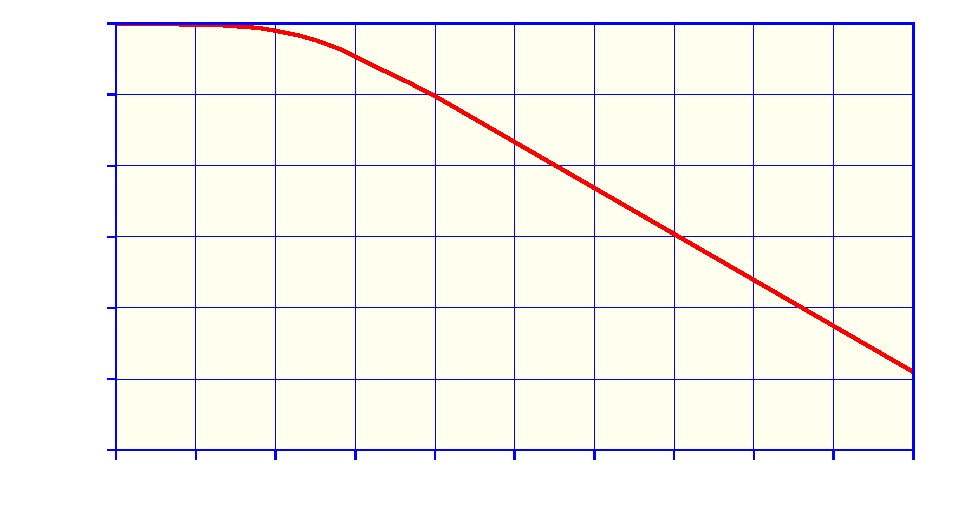
\includegraphics{Cap-Motors-Induccio-U-Deseq}}%
    \gplfronttext
  \end{picture}%
\endgroup

    \captionof{figure}{Tensió d'alimentació desequilibrada en motors. NEMA MG-1}
    \label{pic:Du-kp-ki}
\end{center}


\begin{exemple}[Tensió d'alimentació desequilibrada en un motor segons NEMA MG-1]\label{ex:NEMA-tens-deseq}
	\addcontentsxms{Tensió d'alimentació desequilibrada en un motor segons NEMA MG-1}
Es tracta de trobar el factor $\kappa\ped{P}$  i el valor de la potència nominal corregida, en els dos casos següents:	
    \begin{enumerate}
		\renewcommand{\labelenumi}{\alph{enumi})}
		\item Un motor de  potència nominal: $P\ped{m,n} = \qty{7,5}{HP}$, alimentat per tres tensions de fase desequilibrades   de valors: 460 V, 467 V i 450 V.
		
		\item El motor de l'exemple \vref{ex:mot-tens-deseq}.
	\end{enumerate}
	
	a)  En aquest cas, el valor mitjà de la tensió val:
    \[
      \bar{U} = \frac{\qty{460}{V}+\qty{467}{V}+\qty{450}{V}}{3} = \qty{459}{V}
    \]

    La màxima desviació de les tres tensions respecte d'aquest valor és: $\qty{459}{V}-\qty{450}{V} = \qty{9}{V}$. Per tant tenim:
    \[
        \Deltaup u = \frac{\qty{9}{V}}{\qty{459}{V}} = \num{0,02} = \qty{2}{\%}
    \]

     A partir d'aquest valor, trobem a la Figura \vref{pic:Du-kp-ki} el valor:  $\kappa\ped{P} = \num{0,95}$.

     Per tant, haurem de reduir la potència nominal a:
     \[
         P'\ped{m,n} = \num{0,95}\times{}P\ped{m,n}  = \num{0,95}\times\qty{7,5}{HP} = \qty{7,1}{HP}
     \]
     
	 b)  En aquest cas, el valor mitjà de la tensió val:
	 \[
	 \bar{U} = \frac{\qty{399}{V}+\qty{370}{V}+\qty{370}{V}}{3} = \qty{379,7}{V}
	 \]
	 
	 La màxima desviació de les tres tensions respecte d'aquest valor és: $\qty{399}{V}-\qty{379,7}{V} = \qty{19,3}{V}$. Per tant tenim:
	 \[
	 \Deltaup u = \frac{\qty{19,3}{V}}{\qty{379,7}{V}} = \num{0,05} = \qty{5}{\%}
	 \]
	 
	 A partir d'aquest valor, trobem a la Figura \ref{pic:Du-kp-ki} el valor:  $\kappa\ped{P} = \num{0,76}$.    
     
     Per tant, haurem de reduir la potència nominal a:
     \[
     P'\ped{m,n} = \num{0,76}\times{}P\ped{m,n}  = \num{0,76}\times\qty{9052,8}{W} = \qty{6880,1}{W}
     \]
\end{exemple}

\subsection{Classes d'aïllaments tèrmics en motors}
\index{NEMA!MG-1!classes d'a\"{i}llaments tèrmics}

Quan es posa en marxa un motor, la seva temperatura comença a pujar
per sobre de la temperatura ambient a causa del corrent que circula
pels seus debanats.

La norma NEMA MG-1 defineix diverses classes d'aïllament tèrmic, depenent de
l'increment global de temperatura permès respecte de la temperatura
ambient, que fixa en \qty{40}{\degreeCelsius};\index{temperatura!ambient}
per a cada classe es permet un increment addicional de temperatura
en el punt més calent, situat en el centre dels debanats del
motor. En la Taula \vref{taula:classes-nema} es donen les classes d'aïllament existents.

\begin{center}
   \captionof{table}{Classes NEMA d'aïllaments tèrmics en motors} \label{taula:classes-nema}
   \begin{tabular}{cr<{\hspace{6em}}r<{\hspace{8em}}}
   \toprule[1pt]
   Classe & \multicolumn{1}{c}{Increment global de temperatura} & \multicolumn{1}{c}{Increment addicional de temperatura} \\
   NEMA &   \multicolumn{1}{c}{sobre la temperatura ambient}  & \multicolumn{1}{c}{en el punt més calent} \\
   \midrule
   A & \qty{60}{\degreeCelsius} & \qty{5}{\degreeCelsius}   \\
   B & \qty{80}{\degreeCelsius} & \qty{10}{\degreeCelsius}   \\
   F & \qty{105}{\degreeCelsius} & \qty{10}{\degreeCelsius}   \\
   H & \qty{125}{\degreeCelsius} & \qty{15}{\degreeCelsius}   \\
   \bottomrule[1pt]
   \end{tabular}
\end{center}
\index{A} \index{B} \index{F} \index{H}



\section{Compatibilitat entre els motors de 50 Hz i els de 60 Hz}\label{sec:motors-50-60}

Com és sabut, hi ha dues freqüències de generació de tensió en tot el món, \qty{50}{Hz} i \qty{60}{Hz}. A l'Àfrica, Àsia, Europa,  Oceania i la meitat sud d'Amèrica del Sud, la tensió d'ús és la de \qty{50}{Hz}, amb algunes excepcions com ara l'Aràbia Saudita, Corea del Sud, les Filipines o Taiwan. Al Canadà, als Estats Units, Amèrica Central i la meitat nord  d'Amèrica del Sud, la tensió d'ús és la de \qty{60}{Hz}, amb l'excepció de la Guaiana francesa o algunes petites illes caribenyes. Al Japó coexisteixen les dues freqüències. A l'adreça \href{https://en.wikipedia.org/wiki/Mains_electricity_by_country}
{https://en.wikipedia.org/wiki/Mains\_electricity\_by\_country} es pot veure un mapa i un llistat detallat dels voltatges i freqüències utilitzats en cada país.

Hem vist en els apartats anteriors que la tensió afecta el comportament del motor, i també sabem que la freqüència de la tensió en determina la velocitat. Un altre concepte important, però, és el flux magnètic $\phi$ al qual està sotmès el motor; aquest flux és proporcional al quocient entre la tensió $U$ i la freqüència $f$:
\begin{equation}
	\phi \propto \frac{U}{f}
\end{equation}

Cada motor està dissenyat per a un valor de flux determinat, i augmentar-lo  o disminuir-lo ocasiona que el motor deixi de funcionar segons les seves característiques nominals. En general, el que és més perjudicial per al motor és un augment del flux, ja que això ocasiona un  augment de la temperatura.

Tal com s'ha dit en els apartats anteriors, el parell mecànic és proporcional al quadrat de la tensió. Si ara tenim en compte a més que la freqüència pot variar, caldrà tenir en compte a més, que el parell mecànic és inversament proporcional al quadrat de la freqüència:
\begin{equation}
	T\ped{m} \propto {\left(\frac{U}{f}\right)}^2
\end{equation}

D'aquesta relació es desprèn que si la relació $U/f$ es manté constant, el parell mecànic també es mantindrà constant. En general, la relació entre el parell mecànic $T\ped{m,1}$ desenvolupat a una tensió $U_1$ i a una freqüència $f_1$, i el parell mecànic $T\ped{m,2}$ desenvolupat a una tensió $U_2$ i a una freqüència $f_2$, és:
\begin{equation}\label{eq:Tm_U_f}
	\frac{T\ped{m,1}}{T\ped{m,2}}={\left(\frac{{U}_{1}}{{U}_{2}}\frac{{f}_{2}}{{f}_{1}}\right)}^2
\end{equation}

Pel que fa a la velocitat mecànica, donat que és proporcional a la freqüència, la relació entre la velocitat mecànica $\omega\ped{m,1}$ o $n\ped{m,1}$ desenvolupada a una freqüència $f_1$, i la velocitat mecànica $\omega\ped{m,2}$ o $n\ped{m,2}$ desenvolupada a una freqüència $f_2$, és:
\begin{equation}\label{eq:nm_U_f}
	\frac{\omega\ped{m,1}}{\omega\ped{m,2}} = \frac{n\ped{m,1}}{n\ped{m,2}} = \frac{f_1}{f_2}
\end{equation}

Respecte a la  potència mecànica, donat que  és igual al producte del parell mecànic per la velocitat mecànica, la relació entre la potència mecànica $P\ped{m,1}$ desenvolupada a una tensió $U_1$ i a una freqüència $f_1$, i la potència mecànica $P\ped{m,2}$ desenvolupada a una tensió $U_2$ i a una freqüència $f_2$, és:
\begin{equation}\label{eq:Pm_U_f}
	\frac{P\ped{m,1}}{P\ped{m,2}} =
	{\left(\frac{{U}_{1}}{{U}_{2}}\frac{{f}_{2}}{{f}_{1}}\right)}^2
	\frac{f_1}{f_2} = 	
	 {\left(\frac{{U}_{1}}{{U}_{2}}\right)}^{2} \frac{{f}_{2}}{{f}_{1}}
\end{equation}

Finalment, donat que les potències mecànica i elèctrica estan relacionades pel rendiment segon l'equació \eqref{eq:mot-rendim}, i que el corrent absorbit està relacionat amb la potència elèctrica i el factor de potència segon l'equació \eqref{eq:mot-P}, la relació entre el corrent absorbit $I_{1,1}$  a una tensió $U_1$ i a una freqüència $f_1$, i el corrent absorbit $I_{1,2}$ a una tensió $U_2$ i a una freqüència $f_2$, és:
\begin{equation}
	\frac{I_{1,1}}{I_{1,2}} =
	\frac{U_1}{U_2} \frac{f_2}{f_1} \frac{\cos\varphi_2}{\cos\varphi_1} \frac{\eta_2}{\eta_1}
\end{equation}

Els rendiments i factors de potència varien poc pel valor de corrent nominal, i per tant tenim que la relació entre el corrent nominal absorbit $I\ped{n,1}$  a una tensió $U_1$ i a una freqüència $f_1$, i el corrent nominal absorbit $I\ped{n,2}$ a una tensió $U_2$ i a una freqüència $f_2$, és:
\begin{equation}\label{eq:In_U_f}
	\frac{I\ped{n,1}}{I\ped{n,2}} \approx
	\frac{U_1}{U_2} \frac{f_2}{f_1}
\end{equation}

\begin{exemple}[Variació dels paràmetres d'un motor amb la tensió i la freqüència]
	\addcontentsxms{Variació dels paràmetres d'un motor amb la tensió i la freqüència}
	Tenim un motor amb els següents paràmetres nominals: $U=\qty{460}{V}$, $f=\qty{60}{Hz}$,  $P\ped{m}=\qty{1}{HP}$ i $n\ped{m}=\qty{1725}{r/min}$. Si connectem aquest motor a una xarxa de: $U=\qty{380}{V}$ i $f=\qty{50}{Hz}$, es tracta de calcular els nous valors nominals del motor.
	
	Utilitzarem el subíndex «1» per a les magnituds  a \qty{50}{Hz} i el  subíndex «2» per a les magnituds a \qty{60}{Hz}.
	
	Les relacions entre tensions i freqüències,  són:
	\[
		\frac{U_1}{f_1} = \frac{\qty{380}{V}}{\qty{50}{Hz}} = \qty{7,6}{V/Hz} \qquad \qquad
		\frac{U_2}{f_2} = \frac{\qty{460}{V}}{\qty{60}{Hz}} = \qty{7,7}{V/Hz} 
	\]

	Utilitzant les equacions \eqref{eq:Tm_U_f},  \eqref{eq:nm_U_f}, \eqref{eq:Pm_U_f} i \eqref{eq:In_U_f},  tenim:
	\begin{align*}
		\frac{T\ped{m,1}}{T\ped{m,2}} &= {\left(\frac{\qty{380}{V}}{\qty{460}{V}}\frac{\qty{60}{Hz}}{\qty{50}{Hz}}\right)}^2 = \num{0,98} \\[1ex]
		\frac{n\ped{m,1}}{n\ped{m,2}} &= \frac{\qty{50}{Hz}}{\qty{60}{Hz}} = \num{0,83}  \quad \Rightarrow \quad n\ped{m,1} = \num{0,83} \times \qty{1725}{r/min} = \qty{1437,5}{r/min} \\[1ex]
		\frac{P\ped{m,1}}{P\ped{m,2}} &= {\left(\frac{\qty{380}{V}}{\qty{460}{V}}\right)}^{2} \frac{\qty{60}{Hz}}{\qty{50}{Hz}} = \num{0,82} \quad \Rightarrow \quad P\ped{m,1} = \num{0,82} \times \qty{1}{HP} = \qty{0,82}{HP}\\[1ex]
		\frac{I\ped{n,1}}{I\ped{n,2}} &\approx
		\frac{\qty{380}{V}}{\qty{460}{V}} \frac{\qty{60}{Hz}}{\qty{50}{Hz}} = \num{0,99}
	\end{align*}

	El fet que les dues relacions tensió--freqüència siguin molt similars, fa que la relació entre els parells i la relació entre els corrents siguin properes a 1. La relació entre les velocitats i la relació entre les potències, en canvi, són menors que 1 perquè estan condicionades  a la relació de freqüències. 
\end{exemple}

Per a un motor dissenyat per a una freqüència de \qty{60}{Hz} i connectat a una xarxa de freqüència \qty{50}{Hz}, podem dir en general:
\begin{itemize}
	\item El motor girarà més lentament, donat que la freqüència ha disminuït.
	\item Si el motor és autorefrigerat amb ventilador, la disminució de velocitat afectarà negativament a la refrigeració.
	\item Si disminuïm la tensió  per tal de mantenir la relació $U/f$ constant, mantindrem els valors del parell i del corrent, i disminuirem el valor de la potència. Si necessitem més potència caldrà escollir un motor de potència nominal superior. 	
\end{itemize}

Per a un motor dissenyat per a una freqüència de \qty{50}{Hz} i connectat a una xarxa de freqüència \qty{60}{Hz}, podem dir en general:
\begin{itemize}
	\item El motor girarà més ràpidament, donat que la freqüència ha augmentat.
	\item L'augment de velocitat pot  afectar negativament als coixinets  del motor.
	\item Si augmentem la tensió per tal de mantenir la relació $U/f$ constant, mantindrem els valors del parell i del corrent, i augmentarem el valor de la potència. Cal comprovar que aquest augment de tensió està dins dels marges de funcionament del motor.	
\end{itemize}